\documentclass{article}
\usepackage{caption}
\usepackage{geometry}
\usepackage{amsmath}
\usepackage{tikz}
\usepackage{pgfplots}
\pgfplotsset{compat=1.18}
\usepackage{float}
\usepackage{url}
\usepackage{xcolor}
\usetikzlibrary{positioning}
\usetikzlibrary{angles,quotes}
\setlength{\parindent}{0pt}


\newgeometry{outer=2cm, inner=2.5cm, bottom=4cm, top=2.5cm}



\title{\textbf{L'influence du poids dans le ski de fond (TM)}}
\author{Magnus Wenzel}
\date{Février 2026}

\begin{document}


\maketitle

\section{Introduction}

En tant que fondeur de haut niveau, j'entends souvent la phrase suivante: "Il était aussi rapide que moi dans les descentes, alors que je suis plus lourd que lui, j'avais donc forcément de moins bons skis". Ce propos proclame donc qu'implicitement le poids a une influence sur la vitesse de glisse en descente, et que plus quelqu'un est lourd, plus il va avoir de vitesse.
\newline Il est vrai qu'en coupe du monde, certains et certaines athlètes plus légers que la moyenne de coupe du monde disent aussi qu'ils sont plus lents que les autres et aussi que leurs collègues de nation, qui ont le même fart sous les skis.

\section{But}

Cette hypothèse n'a cependant jamais été vérifiée et c'est pour cela que cette thématique m'intrigue quand même. L'hypothèse repose pour l'instant surtout sur des croyances populaires. 
\newline Le but de ce travail de maturité sera donc dans un premier temps de voir si le poids a en effet une influence sur la glisse et si oui, de quel ordre de grandeur est cette influence.  



\section{Théorie en conditions parfaites}

Nous allons dans un premier temps voir si cette hypothèse peut être vérifiée théoriquement. Pour cela, il faut d'abord rappeler les concepts physiques qui entrent en jeu sur le mouvement d'un skieur:

\subsection{Constante d'accélération de la pesanteur $g$}
$g$ est l'accélération qu'un objet subit vers le centre d'un corps massif, comme une planète. Ce n'est proprement parlant pas une constante, car elle dépend de la masse et du rayon du corps, mais comme les expériences ont toutes été faites sur terre, nous pouvons considérer $g$ une constante et de valeur $9,81[\frac{m}{s^2}]$.



\subsection{MRUA}
Dans des conditions parfaites, le mouvement d'un skieur sur un plan incliné est un \textbf{M}ouvement \textbf{R}ectiligne \textbf{U}niformément \textbf{A}ccéléré. Je vais donc ici énumérer les différentes formules associées au MRUA en guise de rappel:
\begin{itemize}
    \item Pour trouver la vitesse $v$ qu'un objet atteint au bout d'un certain temps:
        \begin{equation}
        \label{vit_MRUA}    
        v = v_0+at
        \end{equation}
    où:
    \begin{itemize}
            \item $v$ est la vitesse en $[\frac{m}{s}]$ atteinte à l'arrivée
            \item $v_0$ est la vitesse en $[\frac{m}{s}]$ au départ
            \item $t$ est le temps nécessaire pour le trajet du départ à l'arrivée
            \item $a$ est l'accélération constante en $[\frac{m}{s^2}]$
    \end{itemize}

    \vspace{0.4cm}

    \item Pour trouver le temps $t$ qui est la durée du trajet:
        \begin{equation}
        \label{tem_MRUA_short}    
        t=\frac{v-v_0}{a}
        \end{equation}
        Cette équation est tout simplement l'équation \ref{vit_MRUA}, manipulée de sorte que t est la variable qui ressort.
        \vspace{0.4cm}
    
    \item Pour trouver la distance $d$ qu'un objet parcours par rapport à un point d'origine:
        \begin{equation}
        \label{dis_MRUA_long}    
        x=x_0+v_0t+\frac{at^2}{2}
        \end{equation}
        ou encore:
        \begin{equation}
        \label{dis_MRUA_short}    
        x=x_0+\frac{v^2-v_0^2}{2a}
        \end{equation}
        où:
        \begin{itemize}
            \item $x$ est la distance en $[m]$ à l'arrivée par rapport à un point d'origine
            \item $x_0$ est la distance en $[m]$ au départ par rapport au même point d'origine
            \item $v_0$ est la vitesse en $[\frac{m}{s}]$ au départ
            \item $v$ est la vitesse en $[\frac{m}{s}]$ atteinte à l'arrivée
            \item $t$ est le temps nécessaire pour le trajet du départ à l'arrivée
            \item $a$ est l'accélération constante en $[\frac{m}{s^2}]$
            
        \end{itemize}
        On peut aussi exprimer ces équations en fonction de la distance nette entre $d_0$ et $d$ qui s'appelle $\Delta d$. Logiquement donc, $d = x-x_0$. $d$ est aussi exprimé en [m].
        \newline Les deux équations nous sont utiles car dans la \ref{dis_MRUA_long}, nous n'avons pas besoin de la vitesse finale $v$, et dans la \ref{dis_MRUA_short}, c'est le temps $t$ qui n'est pas nécessaire pour le calcul. Nous allons voir que les deux vont nous être assez utile dans la suite.
        \vspace{0.4cm}

    \item Pour trouver l'accélération constante de l'objet:
        \begin{equation}
        \label{acc_MRUA_short}    
        a = \frac{v-v_0}{t}
        \end{equation}
        ou encore:
        \begin{equation}
        \label{acc_MRUA_long}    
        a = \frac{v^2-v_0^2}{2(x-x_0)}
        \end{equation}
        Ici, l'équation \ref{acc_MRUA_short} est simplement une manipulation algébrique de l'équation \ref{vit_MRUA} et l'équation \ref{acc_MRUA_long} est une manipulation algébrique de l'équation \ref{dis_MRUA_short}.
    \vspace{0.4cm}
    
\end{itemize}


\subsection{2{ème} loi de Newton}

La 2ème loi de Newton est sans doute une des lois les plus connues en physique. C'est la fameuse loi qui dit que la somme des forces est égale à la masse multipliée par l'accélération, ou: 
\begin{equation}
\label{2nd-N}
\sum \vec{F} = m\vec{a}
\end{equation}
\begin{itemize}
    \item où:
    \begin{itemize}
        \item $\vec{F}$ est le vecteur résultant de l'ensemble des forces, dont la norme est en $[N]$, qui s'appliquent sur un objet
        \item $m$ est la masse en $[kg]$ de l'objet
        \item $\vec{a}$ est le vecteur accélération, dont la norme est en $[\frac{m}{s^2}]$, de même sens que la résultante des forces    
    \end{itemize}
\end{itemize}
Cette loi s'applique, contrairement au MRUA, à des forces qui sont de directions différentes, dans ce TM toujours sur un plan 2 dimensionnel. C'est pour cela que la résultante et l'accélération sont exprimés par des vecteurs. 
\newline Cela ne nous posera cependant pas de problème car c'est là que la trigonométrie interviendra.

% section encore à ameliorer


\subsection{Forces de pesanteur et de soutien}

La Force de pesanteur $\vec{P}$ est la force gravitationnelle qui tire un corps vers le centre de la planète. Comme c'est une Force, elle se calcule en [N]. Pour la calculer, on fait appel à la deuxième loi de Newton et à la constante d'accéleration de la pesanteur $g$. En effet, toute force peut se calculer par $\vec{F} = m\vec{a}$, et l'accleration vers le centre de la terre est $g$, donc: 
\begin{equation}
    \label{Pesant}
    \vec{P}=m\vec{g}
\end{equation}
\begin{itemize}
    \item où:
    \begin{itemize}
        \item $\vec{P}$ est la force de pesanteur dont la norme est en [N]
        \item $m$ est la masse en $[kg]$
        \item $\vec{g}$ est l'accélération vers le centre de la terre et dont la norme est de valeur $9.81 [\frac{m}{s^2}]$
    \end{itemize}
\end{itemize}

Il faut noter que comme $\vec{P}$ et $\vec{g}$ sont colinéaires, on peut aussi tout simplement multiplier la norme $\vec{g}$ par $m$ pour obtenir la norme de $\vec{P}$.
\newline Cependant, il faut faire usage des vecteurs pour comprendre la force de soutien $\vec{S}$. C'est la force qu'exerce le sol sur un objet en reaction à sa force de pesanteur. $\vec{S}$ n'est cependant pas colinéaire à $\vec{P}$ si il y a une pente, car $\vec{S}$ est toujours perpendiculaire à la pente. Dans notre cas, nous pouvons définir $\vec{S}$ comme la composante perpendiculaire au plan de $-\vec{P}$:

\begin{center}
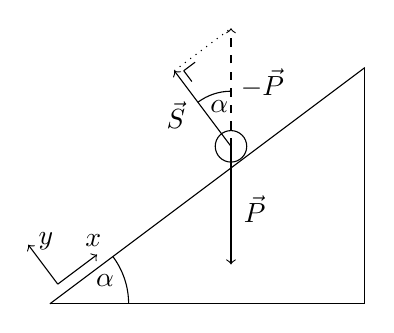
\begin{tikzpicture}
    \draw (1,0) -- (5,3);
    \draw (1,0) -- (5,0);
    \draw (5,3) -- (5,0);
    \draw (3.3,2) circle (0.2);
    \draw[->] (3.3,2) -- (2.58,2.96);
    \draw[->] (3.3,2) -- (3.3,0.5);
    \draw[->, dashed] (3.3,2) -- (3.3,3.5);
    \draw[dotted] (2.58,2.96) -- (3.3,3.5);
    \draw (2.7,2.96) -- (2.844,3.068);
    \draw (2.7,2.96) -- (2.803,2.823);
    \draw (2,0) arc[start angle=0, end angle=36.87, radius=1];
    \draw (3.3,2.7) arc[start angle=90, end angle=126.87, radius=0.7];
    \draw[->] (1.1,0.25) -- (1.6,0.625);
    \draw[->] (1.1,0.25) -- (0.725,0.75);
    
    
    \node at (1.7,0.3) {$\alpha$};
    \node at (3.15,2.5) {$\alpha$};
    \node at (3.6,1.2) {$\vec{P}$};
    \node at (2.6,2.4) {$\vec{S}$};
    \node at (3.7,2.8) {$-\vec{P}$};
    \node at (1.55,0.8) {$x$};
    \node at (0.95,0.8) {$y$};
\end{tikzpicture}
\end{center}

\vspace{0.5cm}

Si ce sont les seules 2 forces qui agissent sur l'objet, ce système n'est pas à l'équilibre. En effet, la force résultante est parallèle au plan (l'axe x), mais pas représentée dans ce schéma afin de le simplifier et car nous ne nous intéressons qu'à la force de pesanteur et de soutien dans cette partie.
Comme $\vec{S}$ est perpendiculaire à la pente, l'angle entre $-\vec{P}$ et $\vec{S}$ est le même que celui entre la pente et le "plat" de la terre. Comme nous avons donc un angle droit et un angle $\alpha$, on peut exprimer la norme de $\vec{S}$ en fonction de la norme de $\vec{P}$:
\begin{equation}
    \label{soutien}
    S=P\cos{\alpha}
\end{equation}


\subsection{Forces de frottements et coefficient de frottement cinétique}

Pour trouver les forces de frottements qu'une surface exerce sur l'autre, il existe une loi qui utilise la force de soutien, que nous pouvons calculer à partir de la masse du skieur et de la pente de la descente. Cette loi dit tout simplement que les forces de frottements sont la force de soutien, multipliée par un facteur de proportionnalité appelé $\mu$:
\begin{equation}
    \label{Coef-frotte-cin}
    F_f = S\mu
\end{equation}
où:
\begin{itemize}
    \item $F_f$ sont les forces de frottements
    \item $S$ est la force de soutien
    \item $\mu$ est le coefficient
\end{itemize}

Ce coefficient varie fortement selon les surfaces mais se trouve généralement entre 0 et 1.



% section encore à ameliorer



\subsection{Utilisation des concepts physiques}

Pour comprendre ce que l'on va faire dans nos calculs, il faut d'abord se faire un schéma global de nos expériences. Sur ce schéma:

\vspace{0.5cm}
\noindent
\begin{minipage}{0.4\textwidth}
\begin{center}
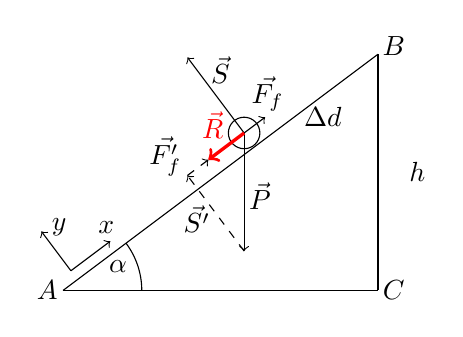
\begin{tikzpicture}
    \draw (1,0) -- (5,3);
    \draw (5,3) -- (5,0);
    \draw (5,0) -- (1,0);
    \draw (3.3,2) circle (0.2);
    \draw[->] (3.3,2) -- (3.3,0.5);
    \draw[->] (3.3,2) -- (2.58,2.96);  
    \draw[->, dashed] (3.3,0.5) -- (2.58, 1.46);
    \draw[->] (3.3,2) -- (3.566666,2.2);
    \draw[->, dashed] (2.58, 1.46) -- (2.84666,1.66);
    \draw[->, very thick, red] (3.3,2) -- (2.84666,1.66);
    \draw (2,0) arc[start angle=0, end angle=36.87, radius=1];
    \draw[->] (1.1,0.25) -- (1.6,0.625);
    \draw[->] (1.1,0.25) -- (0.725,0.75);
    
    
    \draw node at (0.8,0) {$A$};
    \draw node at (5.2,3.1) {$B$};
    \draw node at (5.2,0) {$C$};
    \draw node at (4.3,2.2) {$\Delta d$};
    \draw node at (5.5,1.5) {$h$};
    \node at (1.7,0.3) {$\alpha$};
    \node at (3.5,1.2) {$\vec{P}$};
    \node at (3,2.8) {$\vec{S}$};
    \node at (3.6,2.5) {$\vec{F_f}$};
    \node at (2.9,2.1) {\textcolor{red}{\textbf{$\vec{R}$}}};
    \node at (2.7,0.9) {$\vec{S'}$};
    \node at (2.3,1.7) {$\vec{F_f'}$};
    \node at (1.55,0.8) {$x$};
    \node at (0.95,0.8) {$y$};
    
\end{tikzpicture} 
\end{center}
\end{minipage}
\hfill
\begin{minipage}{0.6\textwidth}
\begin{itemize}
    
    \item $\vec{P}$ est la force de pesanteur du skieur, qui a la même direction que le rayon de la terre et dont le sens est vers le noyau de la terre 
    \item $\vec{S}$ est la force de soutien qu'exerce le sol sur le skieur, de direction perpendiculaire au sol, et dont le sens est "vers le ciel"
    \item $\vec{F_f}$ est la force de frottement de la neige, de direction parallèle au sol et de sens opposé à celui du skieur
    \item $\vec{R}$ est la force résultante, de direction parallèle au sol et de même sens que celui du skieur.
    \item $\vec{S'}$ est l'image de $\vec{S}$ dont le début a été placé à l'extrémité de $\vec{P}$, de même direction, sens, et norme que $\vec{S}$
    \item $\vec{F_f'}$ est l'image de $\vec{F}$ dont le début a été placé à l'extrémité de $\vec{S'}$, de même direction, sens, et norme que $\vec{F_f}$
    \item $\Delta d$ est la distance que parcours le skieur entre $A$ et $B$
    \item $h$ est la hauteur et donc la distance entre $B$ et $C$
    \item $\alpha$ est l'angle entre [AB] et [AC]
\end{itemize}
\end{minipage}

\vspace{0.5cm}


Nous allons maintenant nous intéresser au calcul de l'accélération par voie des forces. Selon la deuxième loi de Newton, la somme des forces est égale à $m\vec{a}$. Dans notre cas les forces sont la force de pesanteur, la force de soutien et les forces de frottement, donc:
\begin{align}
    \nonumber
    \vec{R} = \vec{P} + \vec{S} + \vec{F_f} \\
    \label{ma-somm}
    m\vec{a} = \vec{P} + \vec{S} + \vec{F_f}
\end{align}

Dans le schéma, les vecteurs $\vec{S'}$ et $\vec{F_f'}$ servent à visualiser l'addition. Ce sont des translations des vecteurs originaux. 
\newline Cependant, nous n'utiliserons seulement les normes des vecteurs. Comme, nous pouvons le voir sur le schéma, $\vec{P}$ représente l'hypoténuse, $\vec{F_f'}+\vec{R}$ le côté opposé à l'angle et $\vec{S}$ le côté adjacent. On peut donc continuer nos calculs sans $\vec{S}$ pour le moment:
\begin{align}
    \nonumber
    ma+F_f &= P\sin{\alpha} \\
    \label{ma-Pes-frott}
    ma &= P\sin{\alpha} - F_f
\end{align}

Si l'on appliqiue alors les formules \ref{soutien} et \ref{Coef-frotte-cin}, on obtient:
\begin{align}
    \nonumber
    ma &= P\sin{\alpha} - S\mu \\
    \nonumber
    ma &= P\sin{\alpha} - P\cos{\alpha}\mu \\
    \nonumber
    ma &= mg\sin{\alpha} - mg\cos{\alpha}\mu \\
    \label{acc-cond-parf}
    a  &= g(\sin{\alpha}-\cos{\alpha}\mu)
\end{align}

Bien évidemment, nous ne pourrons pas calculer l'accélération de cette manière là dans nos calculs pratiques, nous utiliserons pour cela les vraies mesures comme le temps $t$ et la distance $\Delta d$.
\newline Ce qui est intéressant dans cette formule est qu'elle n'utilise seulement la gravité sur terre, le coefficient de frottement et l'inclinaison de la pente. On peut donc faire le constat qu'\textbf{en conditions parfaites, l'accélération et donc la vitesse du skieur ne dépend pas de la masse de celui-là.}
\vspace{0.3cm}
\newline Cependant, il n'y a jamais de cas parfait en réalité et le mouvement du skieur n'est en effet pas tout-à-fait un MRUA...

\section{Théorie en conditions réalistes}

On peut se demander quel est ou sont les facteurs qui font que la vitesse du skieur dépendent aussi partiellement de la masse de celui-là. La réponse est que ce sont les forces qui viennent "perturber" le mouvements du skieur, donc les forces de resistances, comme par exemple les forces de frottements. Contrairement donc à ce que l'on a vu dans la partie théorique ou l'on a traité du cas parfait, nous allons donc nous intéressés aux cas où ces forces de résistances ne dépendent pas ou ne se font du moins pas augmenter linéairement par la masse. On peut donc à peu près attribuer les forces de resistances dans ce TM à différentes catégories:

\subsection{1) Forces de résistances constantes}
La force de resistance qui reste constante est un cas assez classique dans la physique. On peut s'imaginer que c'est comme si quelqu'un vous retenait par une corde avec toujours la même force. C'est assez trivial à comprendre, la force ne change tout simplement pas, peu importe la vitesse qu'un objet a:

\begin{center}
\begin{tikzpicture}[>=stealth]

\draw[->, thick] (0,0) -- (6,0) node[right] {$v$};
\draw[->, thick] (0,0) -- (0,4) node[above] {$R_e$};

\draw[thick, blue] (0,1.8) -- (5.5,1.8);
\end{tikzpicture}


\begin{itemize}
    \item $R_e$ est la force de resistance
    \item $v$ est la vitesse de l'objet
\end{itemize}
\end{center}

\vspace{0.3cm}
En effet, il n'y aura pas de paramètre vitesse dans la formule pour trouver ce genre de forces de résistance. Les forces de frottements du skieur en conditions parfaites comme vu plus haut sont un parfait exemple d'une force de resistance constante qui, elles, dependent de la masse. Il y a cependant aussi des cas où ces forces ne dépendent pas linéairement de la masse.
\newline On peut aussi faire remarquer que si un objet ne subit seulement une force de résistance constante, il sera toujours en MRUA et n'aura pas de vitesse terminale. 

\vspace{0.3cm}


\subsubsection{Coefficient de frottement en fonction de la pression}

On peut attribuer les prochains cas de forces de frottements à ces forces de résistances qui restent constantes. 
\newline Pour l'instant, nous avons assumé que le coefficient de frottement est le même pour tout-le-monde. Cependant, cela n'est pas tout-à-fait vrai. 
\newline En effet, un coefficient de frottement qui est le même pour tout-le monde n'est seulement valable si les surfaces ne changent pas. Sauf que c'est justement le cas dans le ski: Un ski fonctionne en faisant fondre la neige en-dessous de lui et en "flottant" sur cette toute fine couche qu'il produit. 
\newline Il existe 2 concepts qui vont influencer cette fonte d'eau, et qui dépendent de la masse.

\subsubsection{Baisse du point de fusion en fonction de la pression}

Le premier n'est pas super intuitif et pour pouvoir l'introduire, il faut d'abord définir ce qu'est la pression.
\newline Pour illustrer cela avec un exemple, une personne en chaussures normales applique plus de pression sur la neige qu'une personne de même poids en raquettes. C'est pour cela qu'une personne en raquettes ne s'enfonce pas dans la neige alors qu'une personne en chaussures normales le fait: la neige subit moins de force par petite surface (la pression) si la personne applique son poids avec les raquettes sous les pieds. Logiquement alors, la formule pour la trouver est:

\begin{equation}
    \label{Pression}
    P_r = \frac{F}{S_u}    
\end{equation}

La pression que subit donc le ski sur la neige est celle de la force de soutien, divisée par la surface du ski qui touche la neige:
\begin{align}
    \nonumber
    P_r &= \frac{S}{S_u} \\
    P_r &= \frac{mg\cos{\alpha}}{S_u}
\end{align}

\begin{itemize}
    \item où:
    \begin{itemize}
        \item $P_r$ est la pression en $[Pa]$
        \item $F$ est la force appliquée sur l'objet en $[N]$
        \item $S_u$ est la surface du ski qui touche la neige $[m^2]$
        \item $m$ est la masse du skieur en $[kg]$
        \item $g$ est la constante d'accélération de la pesanteur en $[\frac{m}{s^2}]$
        \item $\alpha$ est l'angle entre la pente et la tangente de la terre
    \end{itemize}
\end{itemize}

La pression sur le ski augmente donc avec la masse. Mais alors qu'est-ce qu'elle va influencer? Au fait, la pression fait baisser le point de fusion de l'eau par la relation de Clausius-Clapeyron. Elle prend en compte le fait que l'eau à l'état liquide est plus dense que l'eau à l'état solide, donc la neige:
\begin{equation}
    \label{Clausius-Clapeyron}
    \frac{dT}{dP} = \frac{T\Delta{V}}{\Delta{H}}
\end{equation}
\begin{itemize}
    \item où
    \begin{itemize}
        \item $\frac{dT}{dP}$ est la différence de température de fusion par pascal en $[\frac{K}{Pa}]$
        \item $\Delta{V}$ est la differnece du volume molaire entre les 2 états (solide et liquide) en $[\frac{m^3}{mol}]$
        \item $\Delta{H}$ est l'enthalpie de fusion molaire en $[\frac{J}{mol}]$
        \item $T$ est la température de fusion de base en $[K]$
    \end{itemize}
\end{itemize}

\vspace{0.2cm}

On peut expliquer cette equation de la manière suivante: Pour chaque pascal (l'unité de la pression) en plus, la température de fusion augmente d'un certain taux (partie gauche): Cette différence de température par pascal est égal à la température de fusion de base (Pour l'eau à une pression de 1 atmospère cette température est d'env. 273K) fois la difference de volume molaire (Le volume molaire est un peu comme la masse volumique, mais inversée et en prenant les moles à la place des kilogrammes: au lieu de définir quelle est la masse d'un certain volume, on va définir quel est le volume d'une mole d'une substance) entre les l'état liquide et solide, tout cela divisé par l'enthalpie de fusion (c'est presque la même chose que la chaleur massique mais encore une fois avec des moles à la place de kilogrammes). Faisons peut-être un petit exemple:

\vspace{0.4cm}

Commençons déjà par calculer la pression qu'un skieur de 80kg applique sur un ski qui touche la neige sur une surface totale de $300[cm^2]$, égale à $0.03[m^2]$, sur du plat, donc avec un angle $\alpha$ de $0^\circ$:
\vspace{0.1cm}
\begin{align}
    \nonumber
    P_r &= \frac{mg\cos{\alpha}}{S_u} \\
    \nonumber
    P_r &= \frac{40*9.81*\cos{0}}{0.03} \\ % 40kg = moitié du poids sur un seul ski
    \nonumber
    P_r &= 13080 [\frac{kg}{m^2}]    
\end{align}

Pour l'eau, l'enthalpie de fusion par mol est de $6010[\frac{J}{mol}]$, le volume molaire à l'état liquide est de env. $18.02*10^{-6}[\frac{m^3}{mol}]$ et à l'état solide de env. $19.7*10^{-6}[\frac{m^3}{mol}]$ et la température de fusion sous 1 atmosphère est de env. $273K$. On peut donc remplacer tout cela dans la formule de Clausius-Clapeyron:

\begin{align}
    \nonumber
    \frac{dT}{dP_r} &= \frac{T\Delta{V}}{\Delta{H}} \\
    \nonumber
    \frac{dT}{dP_r} &= \frac{273(18.02*10^{-6}-19.7*10^{-6})}{6010} \\
    \nonumber
    \frac{dT}{dP_r} &= \frac{-4.586*10^{-4}}{6010} \\
    \nonumber
    \frac{dT}{dP_r} &= 7.6*10^{-8}
\end{align}

Après, il n'y a plus qu'à multiplier tout cela par la pression du ski (C'est en réalité la différence de pression avec la pression atmosphérique, mais vu que le ski subit aussi celle-là, c'est tout simplement la pression subie par le ski):
\begin{align}
    \nonumber
    \Delta{T} &= \frac{dT}{dP}\Delta P \\
    \nonumber
    \Delta{T} &= 7.6*10^{-8}*13080 \\
    \nonumber
    \Delta{T} &= -9.98*10^{-4}[K]
\end{align}
On peut conclure que la température de fusion n'est baissée que d'un taux infinitésimal, qui n'aura donc pas de vraie influence sur une meilleure fonte de l'eau sous le ski. 
\newline De plus, un ski n'est pas plat, il a une certaine courbure. Ce n'est donc pas tout le ski qui touche la neige, mais 2 surfaces aux extrémités du ski: 

\begin{center}
    \begin{figure}[H]
        \centering
        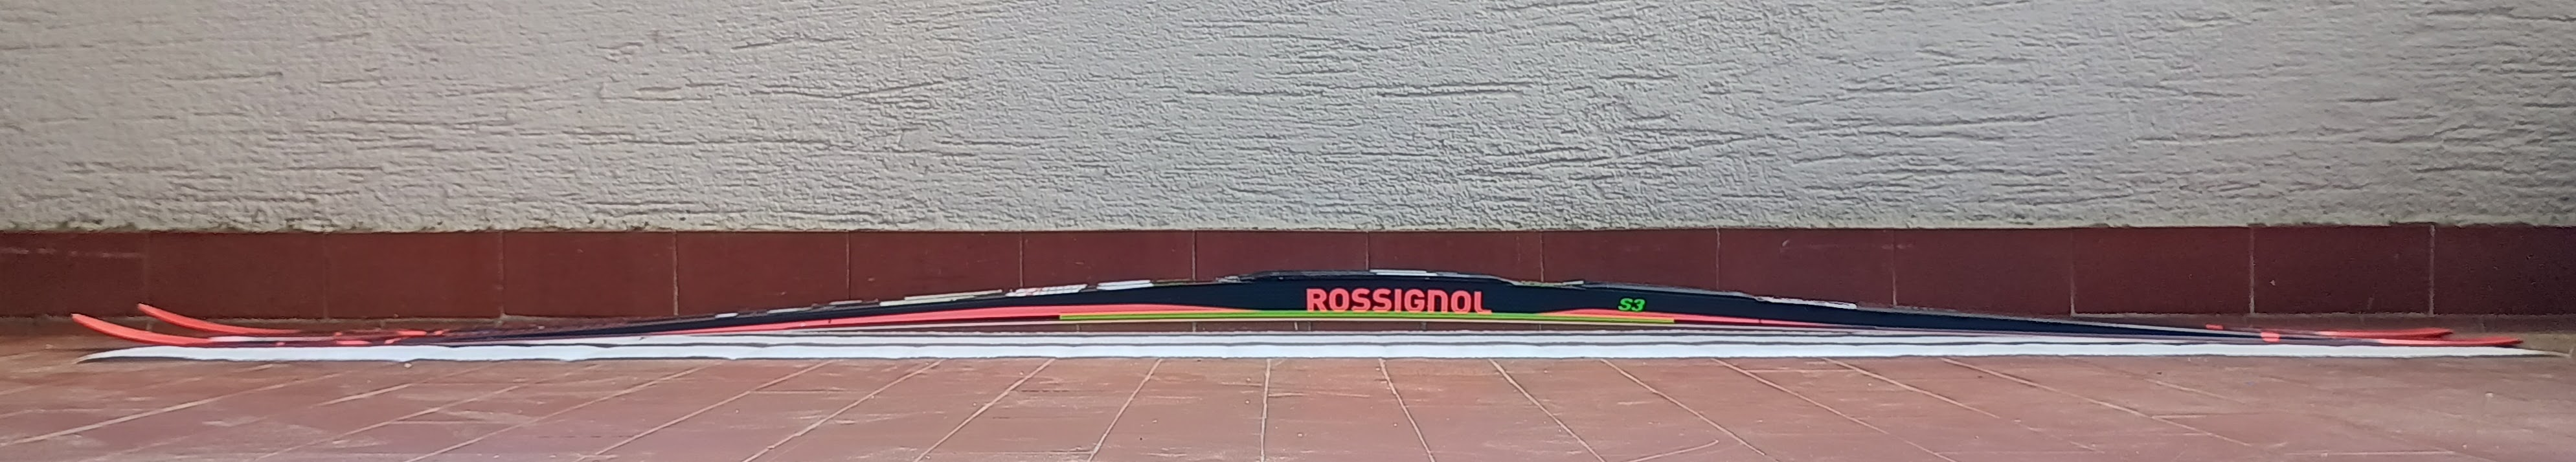
\includegraphics[width=1\linewidth]{Ski_surface_dry/Ski_empty.jpg}
        \caption{Les 2 extrémités du ski sans masse dessus touchent le sol, avec le milieu qui est relevé}
        \label{empty_ski}
    \end{figure}
\end{center}

Si maintenant, L'on pose une masse dessus, le ski s'affaisse, et donc plus de surface touche le sol. La surface du ski augmente donc avec la masse:

\begin{center}
    \begin{figure}[H]
        \centering
        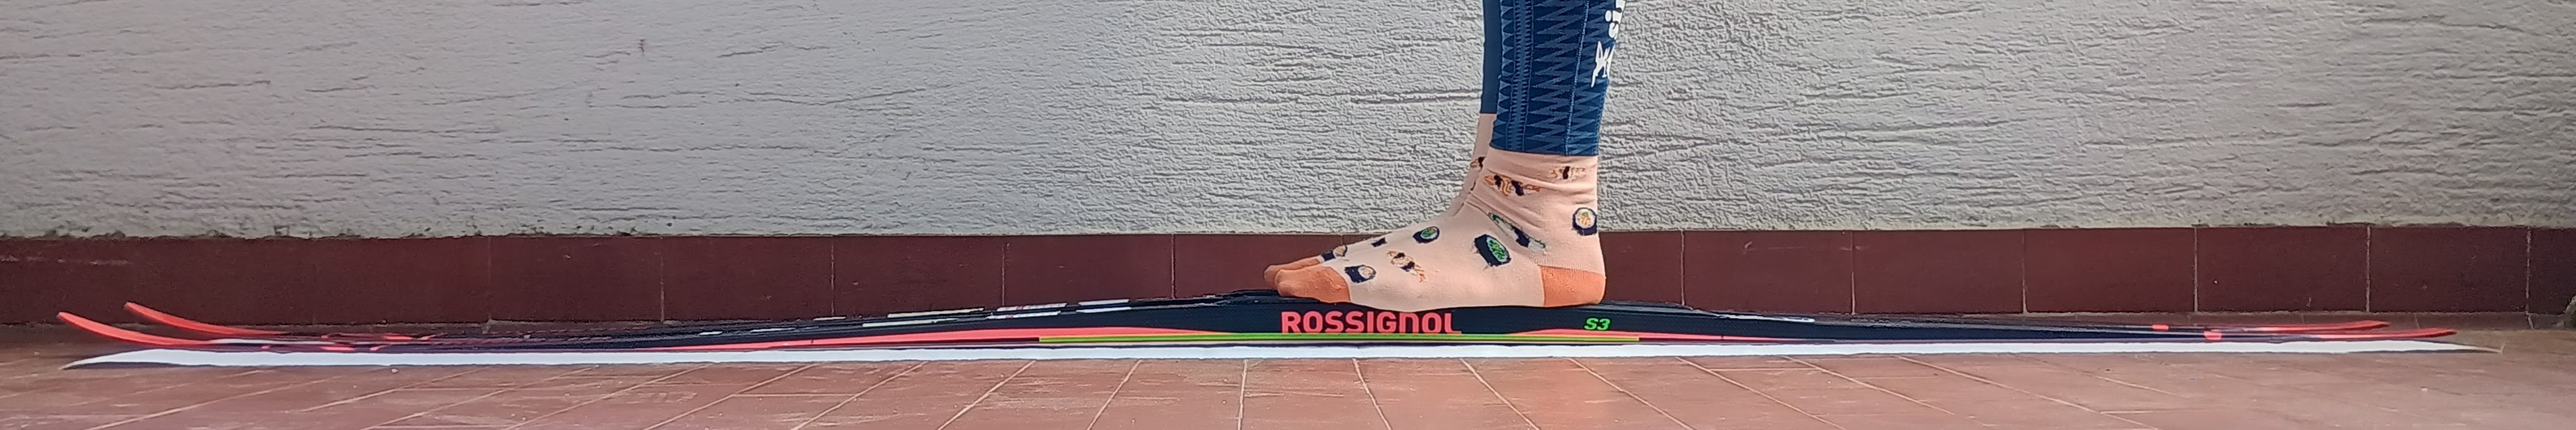
\includegraphics[width=1\linewidth]{Ski_surface_dry/Ski_ella.jpg}
        \caption{Le ski avec une masse de $45[kg]$ dessus}
        \label{dryski_ella}
    \end{figure}
    \begin{figure}[H]
        \centering
        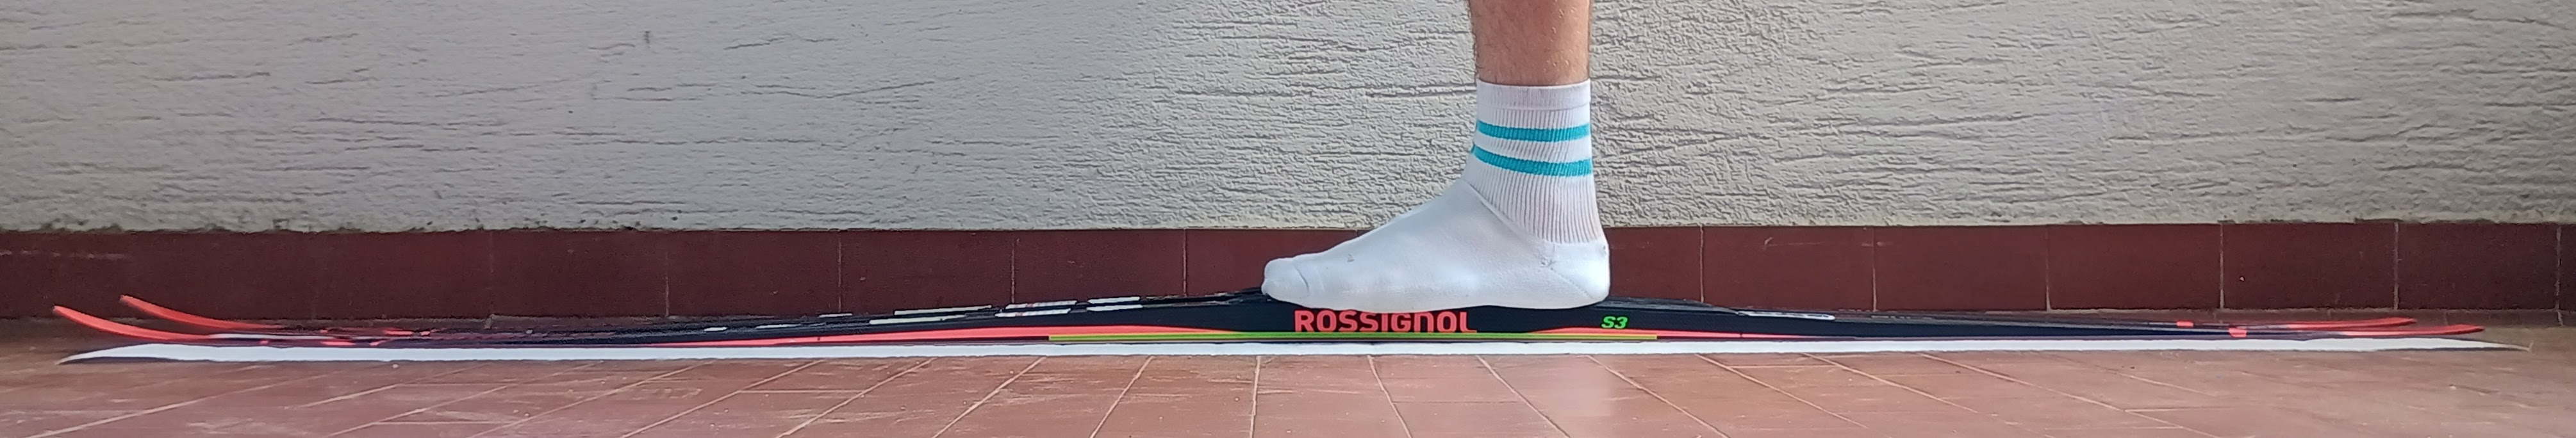
\includegraphics[width=1\linewidth]{Ski_surface_dry/Ski-Magnus.jpg}
        \caption{Le ski avec une masse de $75[kg]$ dessus}
        \label{dryski_magnus}
    \end{figure}
\end{center}

Même si cela est très subtil, on peut observer que la personne de $75[kg]$ fait presque toucher toute la surface du ski sur le sol, alors que pour la personne de $45[kg]$, il y a encore un très leger espace avec le sol au milieu. 
\newline En plus donc que la température de fusion n'est abaissée que d'un miniscule taux, la différence de pression entre les différentes masses est atténuée par le ski qui s'abbaisse et donc fait toucher plus de surface.

\vspace{0.3cm}

\subsubsection{Énergie thermique en fonction des forces de frottements}

Il est important de comprendre que la pression ne fait qu'abaisser le point de fusion. Cette fonte ne se fait du coup que favorisée par plus de pression (donc si un skieur a plus de masse qu'un autre). C'est là qu'arrive le deuxième concept qui influence la fonte d'eau selon la masse: Les forces de frottements qui libèrent de l'énergie thermique qui va faire fondre la neige. 
On a démontré plus haut (equations \ref{Coef-frotte-cin} et \ref{soutien}), que les forces de frottements dépendaient linéairement de la masse. Maintenant, on peut calculer le travail (le "work") que fait les forces de frottements sur toute la longueur de la pente:
\begin{align}
    \nonumber
    W_{F_f} &= F_f \Delta d \\
    \label{Work_forfro}
    W_{F_f} &= mg \mu \Delta d \cos{\alpha}
\end{align}
\begin{itemize}
    \item où:
    \begin{itemize}
        \item $W_{F_f}$ est le travail fourni en $[J]$ par les forces de frottements sur la distance $\Delta d$
        \item $F_f$ sont les forces de frottements en $[N]$ entre la neige et le ski
        \item $\Delta d$ est la distance en $[m]$ sur laquelle les forces de frottements travaillent
        \item $\alpha$ est l'angle entre la pente et la tangente de la terre
        \item $m$ est la masse du skieur en $[kg]$
        \item $g$ est la constante d'accélération de la gravité sur terre de valeur $9.81 [\frac{m}{s^2}]$
    \end{itemize}
\end{itemize}

L'énergie perdue par les forces de frottements est donc, logiquement, proportionnelle à la masse. Maintenant, on ne sait pas quel pourcentage de cette énergie exactement part en énergie thermique, mais on n'a pas besoin de cela. Tant que ce pourcentage est le même pour toutes les masses (ce qu'il est très vraisemblablement), on sait que cette énergie thermique dépend, elle aussi, linéairement de la masse, ce qui veut dire qu'on fait fondre bien plus d'eau en dessous de soi si l'on a une grande masse.

\vspace{0.2cm}

Pour conclure, il y a donc 2 facteurs qui dépendent de la masse qui viennent influencer le coefficient de frottement:
\begin{itemize}
    \item La pression qui, plus elle est grande, fait abaisser le point de fusion de l'eau
    \item Les forces de frottements qui, plus elles sont significatives, créent de l'énergie thermique sous le ski
\end{itemize}

Ces deux concepts tout seul font donc que, en théorie, le coefficient de frottement $\mu$ est réduit chez une personne lourde par rapport à une personne légère. Cependant, en pratique, cela n'est pas toujours le cas. Au fait, cela dépend surtout de l'état de la neige. Si c'est une neige froide et dure, tout ce que j'ai énuméré plus haut est à peu près vrai, comme le montre cette étude:

\begin{center}
    \textit{Influence of Load and Position of Center of Mass on COF in Cross-Country Skiing} \cite{sandberg2025influence}
    \newline (https://link.springer.com/article/10.1007/s11249-025-01999-w) 
\end{center}



Cette étude a été menée dans le premier but de faire ressortir si la position de la masse sur les skis changeait quelque chose au coefficient de frottement, mais ce qui nous intéresse sont les changements de $\mu$ par rapport à la masse. Les expériences dans cette étude consistent à pousser des skis avec la masse dessus à une certaine vitesse et après mesurer leur décélération. Elles ont toutes été faites avec la même neige froide et ce que l'étude a fait ressortir, est que $\mu$ (dans cette étude nommé COF), pouvait être réduit de $15$ pourcents entre une masse de $40[kg]$, et une de $120[kg]$, ce qui est quand même assez significatif:
\begin{center}
    "The results consistently demonstrated that increasing the load on the sled reduced the COF by up to 15 percent (from the lowest to highest load), regardless of the position of the center of mass"
\end{center}
Une autre chose qui m'a marqué est que l'étude montre aussi que le coefficient de frottement se réduisait au fil de la décélération, et donc que les forces de frottements (vu qu'ils sont proportionnels à $\mu$) sont plus grandes à plus grande vitesse:

\begin{center}
    \begin{figure}[H]
        \centering
        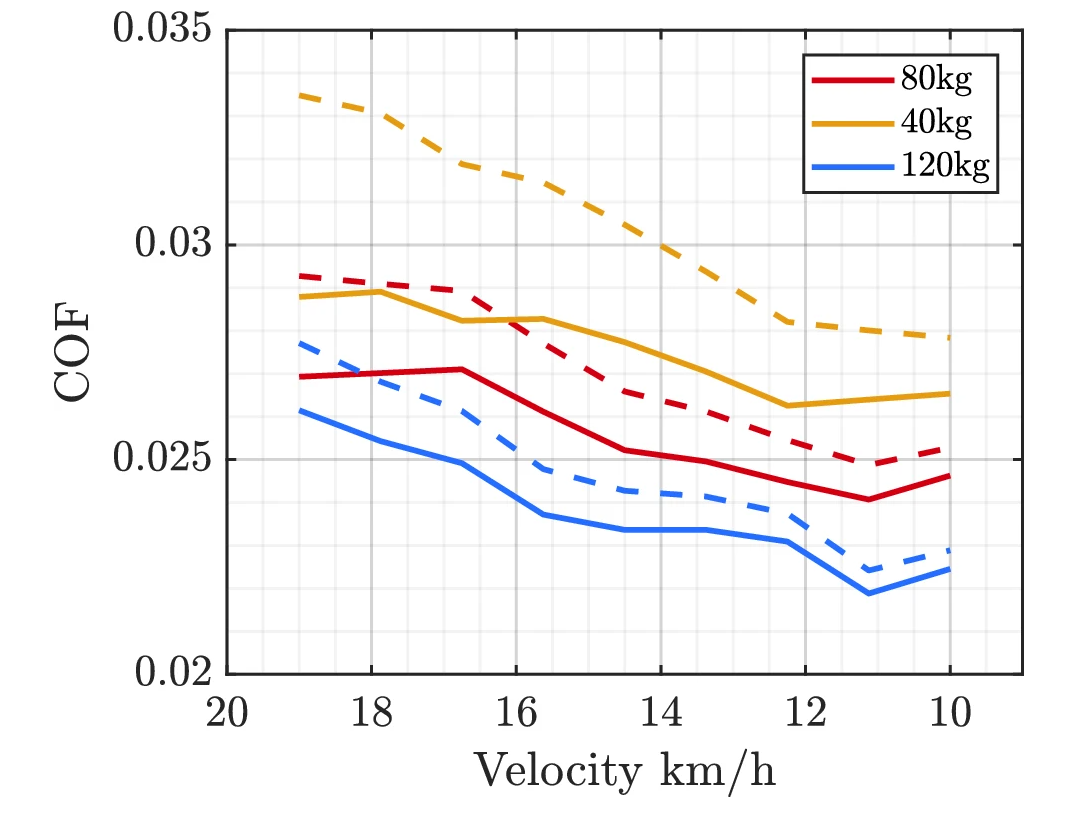
\includegraphics[width=0.8\linewidth]{Influence-of-load(Springer)/Mu-nach-geschwindigkeit.png}
        \caption{$\mu$ d'après la vitesse: Les lignes traitillées négligent les forces de frottements de l'air et les lignes continues sont les coefficients de frottements calculées après avoir pris en compte les frottements de l'air}
        \label{fig:placeholder}
    \end{figure}
\end{center}

Je ne peut pas vraiment expliquer cet effet, et ce n'est pas réellement expliqué dans l'étude non-plus, mais si l'on croit donc ce graphique, il faudrait attribuer ces forces de frottements entre le ski et la neige plutôt au prochain cas, où les forces de frottements augmentent linéairement avec la vitesse.
\newline Une hypothèse qui expliquerait peut-être aussi ce graphique est que le coefficient ne dépend pas de la vitesse du ski, mais de la distance que celui-là parcours, vu que dans leur expérience, le ski décélère au fil de son chemin, et donc la vitesse dépend de la distance qu'il parcours.

\vspace{0.2cm}

Tout cela s'applique donc pour de la neige froide, mais sur l'autre côté, on a la neige molle, qui est en-train de fondre naturellement et est déjà à $0^\circ$. En effet, puisqu'il y a déjà beaucoup d'eau fondue, le ski n'a plus besoin de la faire fondre, et donc tout l'avantage de la masse sur cet aspect là est perdu. Plus de masse est potentiellement même contraproductif, car le ski va plus s'enfoncer dans la neige et l'eau en excès aura un effet ventouse. C'est ce que relèvent certaines autres études que celle de \textit{Springer Nature} cite:

"In contrast, Eriksson reported that COF decreased with increasing pressure for a traditional wooden sled with steel runners on snow, but noted that this relationship only holds true for hard snow surfaces, where deformation of the surface due to increasing load does not occur"* Cet Eriksson a donc fait ces expériences avec une luge (même fonctionnement qu'un ski), et a relevé que la réduction de $\mu$ par la masse était atténuée plus la neige était chaude.

"Buhl et al. conducted experiments on downhill skis and found that, at low temperatures, COF decreased with increasing load. However, this influence diminished as snow temperature rose"
\newline Cette phrase raconte à peu près la même chose que la précédente, sauf qu'eux ont fait les expériences avec des skis alpins.

\vspace{0.2cm}

Pour donc conclure sur la réduction du coefficient de frottement, cette réduction se fait surtout par l'énergie thermique plus grande avec une masse plus significative et en conditions froides. La baisse de la température de fusion par la pression, elle aussi, n'a qu'une influence dans les températures à $0^\circ$, même si elle est tellement petite que presque négligeable. La masse aura donc une plus grande influence sur la vitesse en descente quand la neige est dure que quand la neige est molle.


\subsection{2) Forces de résistances augmentant linéairement en fonction de la vitesse}

Le prochain cas est celui où la force de résistance augemente linéairement par rapport à la vitesse:

\begin{center}
\begin{tikzpicture}[>=stealth]
\draw[->, thick] (0,0) -- (6,0) node[right] {$v$};
\draw[->, thick] (0,0) -- (0,4) node[above] {$R_e$};

\draw[thick, blue] (0,0) -- (5,3);
\end{tikzpicture}
\end{center}

Ce cas est déjà bien plus compliqué car ces forces dépendent de la vitesse.

Plus un objet va vite, plus il est freiné et donc il ne s'agit plus d'une accélération constante, car elle est diminuée au fur et à mesure que la vitesse augmente. En effet, si l'on considère que la force qui fait bouger l'objet, elle, est constante, il existe une vitesse ou la résistance devient tellement grande qu'elle est égale à la force qui fait avancer l'objet. C'est ce que l'on appelle la vitesse terminale. Cette vitesse ne nous intéressera cependant pas plus que ça dans ce TM, car le skieur ne l'atteindra jamais.
\newline Comme nous l'avons vu plus haut, les forces de frottements entre le ski et la neige pourraient être attribuées à ce cas dans certaines conditions de neige spécifiques.



\subsection{3) Forces de résistances augmentant exponentiellement en fonction de la vitesse}

Un cas encore plus compliqué est quand la force de résistance augmente exponentiellement par rapport à la vitesse:

\begin{center}
\begin{tikzpicture}[>=stealth]

% Achsen
\draw[->, thick] (0,0) -- (6,0) node[right] {$v$};
\draw[->, thick] (0,0) -- (0,4) node[above] {$R_e$};

% Exponentielle Funktion
\draw[thick, blue, domain=0:5, smooth, variable=\x]
    plot ({\x},{0.2*exp(0.6*\x)-0.2});
\end{tikzpicture}
\end{center}

Comme dans le cas précédant, il y a ici aussi une vitesse terminale. 
\newline Dans ce cas se range une force de résistance très connue en physique et dont nous devons en prendre compte dans nos expéreinces car omniprésente sur terre:



\subsubsection{Résistances de l'air}

Les frottements de l'air prennent une place de plus en plus importante dans le monde du sport d'endurance. On peut le voir avec les vélos et la position de plus en plus perfectionnés dans le cyclisme, ou encore dans la recherche du tissu le plus aérodynamique pour les skieurs alpins. En ski de fond aussi, et donc dans nos expériences, les résistances de l'air ont une certaine importance. La formule pour trouver les resistances de l'air est la suivante:

\begin{equation}
    \label{Airdrag}
    D = \frac{C \rho A v^2}{2}
\end{equation}

\begin{itemize}
    \item où:
    \begin{itemize}
        \item $D$ est la force de résistance du vent en $[N]$
        \item $C$ est le coefficient de trainée (facteur de proportionnalité)
        \item $\rho$ est la masse volumique de l'air en $[\frac{kg}{m^3}]$
        \item $A$ est la surface séquante en $[m^2]$
        \item $v$ est la vitesse de l'air relative à l'objet en $[m/s]$
    \end{itemize}
\end{itemize}

L'on voit bien ici que la force $D$ augmente exponentiellement par rapport à la vitesse. 
Mais alors d'où vient cette formule? Pour ce faire, il faut s'y approcher par la quantité de mouvement qu'exerce l'air sur le skieur. Cette quantité de mouvement est donc: $\vec{p_a} = m_{a}v_{a}$, avec $p_a$ la quantité de mouvement de l'air, $m_a$ la masse de l'air, et $v$ la vitesse de l'air, relative au skieur, donc la vitesse du skieur. Il faut donc pouvoir déterminer la masse de l'air. La masse, ce n'est rien d'autre que le volume $V$ fois la masse volumique $\rho$:
$$m_a = V\rho$$
Le volume d'air que le skieur bouge donc, est sa surface séquante $A$, fois la distance qu'il fait dans un instant infiniment petit, noté $\Delta L$:
$$m_a = \rho A \Delta{L}$$
Comme tout cela se passe en instantanné, donc un laps de temps $\Delta t$ infiniment petit, on peut encore remplacer la distance par ce temps $\Delta{t}$, fois la vitesse du skieur $v$:
$$m_a = \rho A \Delta{t} v$$

Remplaçons tout cela dans notre équation de quantité de mouvement:
\begin{align}
    \nonumber
    p_a &= (\rho A \Delta{t} v)v \\
    p_a &= \rho A \Delta{t} v^2
\end{align}

Si l'on revient à la définition de la quantité de mouvement, on peut mettre en relation la quantité de mouvement et la force:
$$F=\frac{p}{\Delta t}$$
Si l'on nomme donc force de résistance de l'air $D$, on obtient:
\begin{align}
    \nonumber
    D &= \frac{\rho A \Delta{t} v^2}{\Delta{t}} \\
    \label{drag_perf-cond}
    D &= \rho A v^2
\end{align}

Cela est cependant la formule dans le cas absolument idéal, où la surface séquante est une surface absolument plane, et où l'air qui nous frappe disparait juste après. En réalité, cela est beaucoup plus compliqué, car les molécules sont déviées, passent à côté, sont repoussées etc.. C'est pour cela qu'il existe, un peu comme le facteur de proportionnalité $\mu$ entre 2 surfaces, un facteur de proportionnalité $C$ d'un corps, généralement situé entre 0.4 et 0.6 en chouss chez un skieur de fond et environ à 1 quand il est debout. 
\newline De plus, on divise le tout par 2, ce qui vient de la pression dynamique des équations de Bernoulli (dynamique des fluides). Tout cela ensemble nous donne donc la formule tout en haut:
$$D = \frac{C \rho A v^2}{2}$$

\vspace{0.5cm}

Si l'on revient à la deuxième loi de Newton, $\sum{\vec{F}}=m\vec{a}$, et que l'on ne considère que les forces de frottements de l'air, on peut dire que:
\begin{align}    
    \nonumber
    ma &= mg\sin{\alpha} - \frac{C \rho A v^2}{2} \\
    \label{skier_acc_airdrag}
    a &= g\sin{\alpha} - \frac{C \rho A v^2}{2m} 
\end{align}

On peut donc ici aussi clairement constater que l'accélération, et donc la vitesse du skieur dépend bien de sa masse, juste si on prend on compte les résistances de l'air.


\subsection{Les forces de résistances ensemble}

La masse peut donc influencer l'accélération du skieur par 
\begin{itemize}
    \item La baisse de la température de fusion (Même si minime)
    \item L'énergie perdue par les forces de frottements qui se transforment en énergie thermique
    \item Les frottements de l'air dans lesquels la masse n'a aucune influence
\end{itemize}

Même si l'on ne connait pas de formule pour proprement claculer les forces de frottements entre le ski et la neige, pour calculer l'accélération, cela donne au final cela:
\begin{equation}
    \label{acc-global-real}
    a = g\sin{\alpha} - \frac{C \rho A v^2}{2m} - \frac{F_f}{m}
\end{equation}
\begin{itemize}
    \item où:
    \begin{itemize}
        \item $a$ est l'accélération du skieur en $[\frac{m}{s^2}]$
        \item $g$ est la constante d'accélération de gravité en $[\frac{m}{s^2}]$
        \item $\alpha$ est l'angle entre la pente et la tangente de la terre
        \item $C$ est le coefficient de trainée (facteur de proportionnalité)
        \item $\rho$ est la masse volumique de l'air en $[\frac{kg}{m^3}]$
        \item $A$ est la surface séquante en $[m^2]$
        \item $v$ est la vitesse de l'air relative à l'objet en $[m/s]$
        \item $F_f$ sont les forces de frottements en $[N]$ entre le ski et la neige
        \item $m$ est la masse en $[kg]$ du skieur
    \end{itemize}
\end{itemize}

\vspace{0.2cm}
Cette formule finale fait ressortir que en effet, \textbf{en théorie réaliste, la masse a une influence sur la vitesse du skieur.}
Cette formule ne nous suffira cependant malheureusement pas à calculer par exemple les résistances de l'air où $\mu$, car il y a trop de facteurs inconnus. Nous nous contenterons donc dans les expériences de nous concentrer sur le but principal qu'est de trouver si la masse a une influence ou pas.


\section{Expériences pratiques et analyse des résultats}

Pour répondre à cette question, j'ai pu faire 3 expériences. Une à St. Moritz, une à Pontresina, et une au col des Mosses. Elles sont toutes similaires dans le fond, car elles consistaient toutes à mesurer le temps dont les différents skieurs avaient besoin sur un certain tracé. Il y a tout-de-même quelques différences entre elles, souvent pour essayer de par exemple atténuer une source d'erreur devenue claire à l'expérience d'avant, ou pour varier les conditions des prises de mesure.


\subsection{1ère expérience}

La première expérience se déroula donc à St.Moritz, il faisait $-4^\circ$C, donc des conditions typiques pour le ski de fond, et il venait de neiger (donc des conditions de nouvelle neige). Nous l'avons faite tard dans l'après-midi et le ciel était nuageux, donc le soleil n'avait plus d'influence sur l'expérience.

\subsubsection{Préparation (1)}

\noindent
\begin{minipage}{0.45\textwidth}
Comme donc dit plus haut, les expériences se déroulent toutes comme-cela: on mesure le temps que le skieur a besoin pour descendre une certaine distance d'une certaine pente. La distance et la pente ne sont seulement là comme ordre de grandeur pour indiquer sur quel type de descente nous nous trouvons, car comme mentionné dans la théorie réalistes, il ne nous sera malheureusement pas possible d'en tirer des valeurs comme le coefficient de frottement, ce qui aurait été intéressant, par exemple. 
\newline Pour donc mesurer la longueur du tronçons sur lequel se déroulera l'expérience, j'ai pris une fine corde de 60m et l'ai graduée à l'aide de ma soeur, d'une règle à mesurer et de fils de masque. Grâce à ma soeur qui tendait le fil à marquage d'un côté et moi de l'autre, nous avons marqué chaque mètre d'un point rouge et chaque $5[m]$, d'un noeud fait avec du fil de masque. Nous l'avons après enroulé autour d'un rouleau de papier cuisine vide pour le transporter. 
\newline Une fois arrivé sur place, il n'y avait plus qu'à dérouler le fil et à le tendre entre le bâton qui marquait le départ et le bâton qui marquait l'arrivée.
\newline Nous avons utilisé ce fil pour toutes les expériences.
\end{minipage}
\hfill
\begin{minipage}{0.55\textwidth}
\begin{center}
    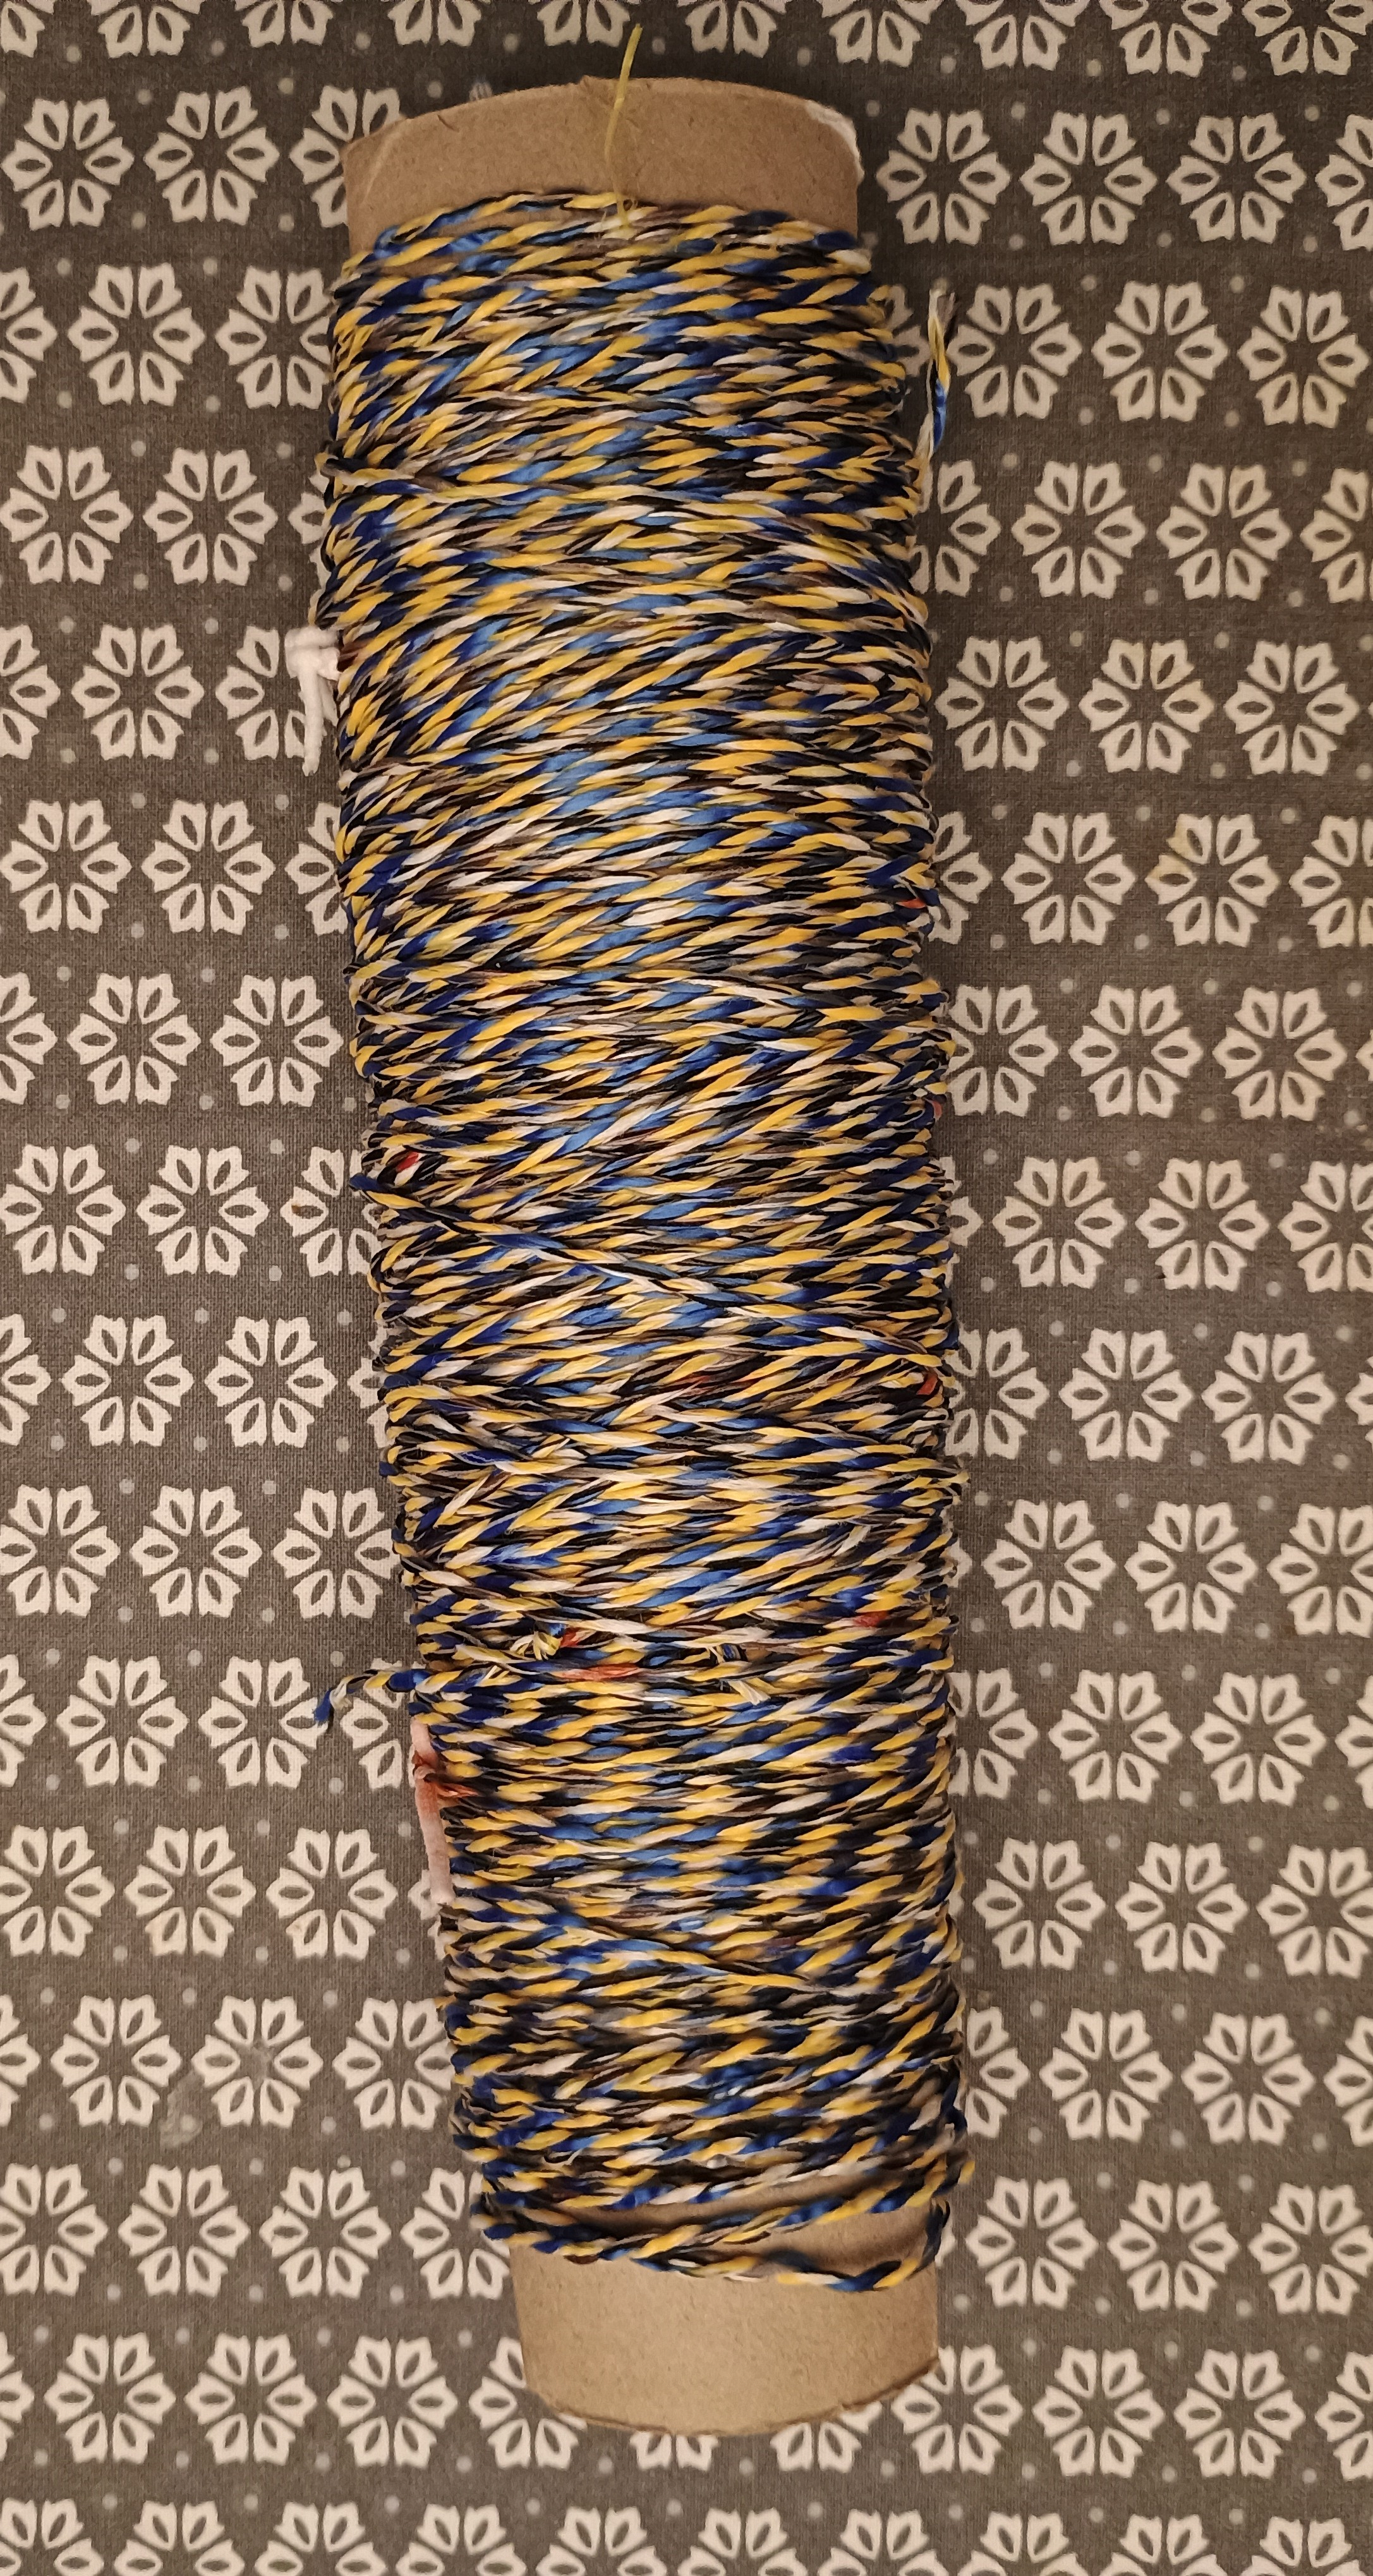
\includegraphics[width=0.75\linewidth]{Exp_1_St.Moritz/Cord_St.Mo.jpg}
    \captionof{figure}{La corde de mesure prête à être utilisée}
    \label{Cord_enroul}
\end{center}
\end{minipage}

\vspace{0.6cm}

Ensuite, il faut bien un endroit approprié pour faire des mesures. Nous nous étions mis d'accords de faire l'expérience tarddans l'après-midi, et donc j'ai pendant le matin cherché une descente appropriée pour les mesures. Mes critères étaient les suivants: il fallait que la descente soit droite, avec le moins de changements de terrains que possible, qui a une certaine longueur, et qui est assez penteuse pour que le skieur avance, mais pas trop pour qu'il y ait quand même un certain temps de déplacement entre le départ et l'arrivée. En plus de cela. il fallait que cette descente ne soit si possible pas sur une piste principale pour éviter que l'expérience ne se fasse pas interrompre par quelqu'un qui passe toute les $3$ secondes
\newline J'ai donc trouvé une telle descente durant la matinée, mais il fallait encore faire une chose: tracer une trace d'expérience nous-même. En effet, comme il avait neigé pendant la nuit d'avant et partie de la matinnée, les traces avaient donc complètement disparues et tout était recouvert d'une couche de neige fraiche.
\begin{figure}[H]
    \centering
    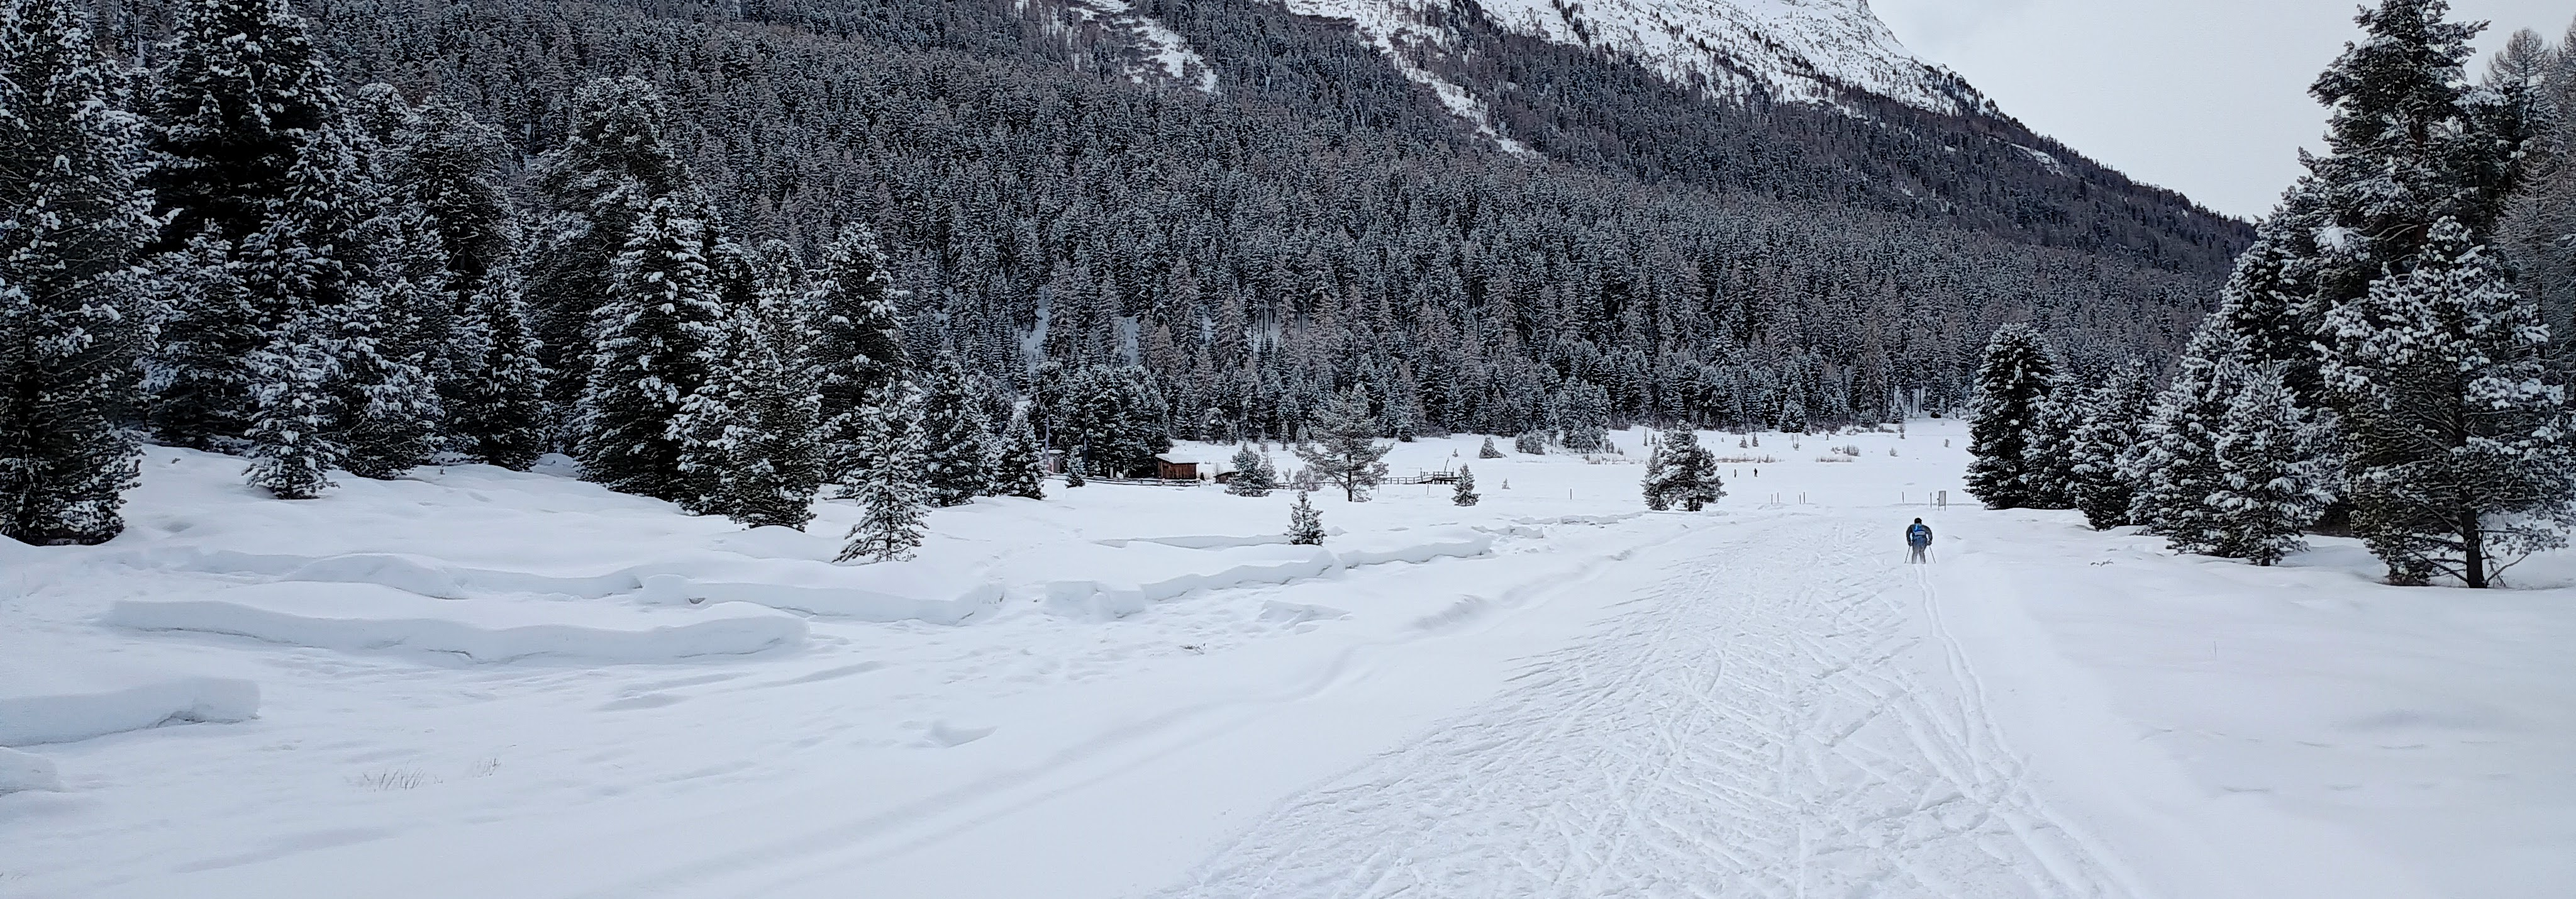
\includegraphics[width=1\linewidth]{Exp_1_St.Moritz/St.Moritz_Powder(3).jpg}
    \caption{Photo prise pendant le tour dans la matinée: On peut y voir la nouvelle neige et que ce sont les fondeurs eux-mêmes qui "tracent" la piste (ceci n'est pas la trace de l'expérience)}
    \label{St.Mo_pow}
\end{figure}

Aussi, afin d'obtenir des mesures comparables entre les skieurs, il faut qu'ils aient tous des conditions de departs égales. Un paramètre qu'il faut pour que ces conditions soient égales, est que le matériel doit être le même.


\begin{minipage}{0.41\textwidth}
        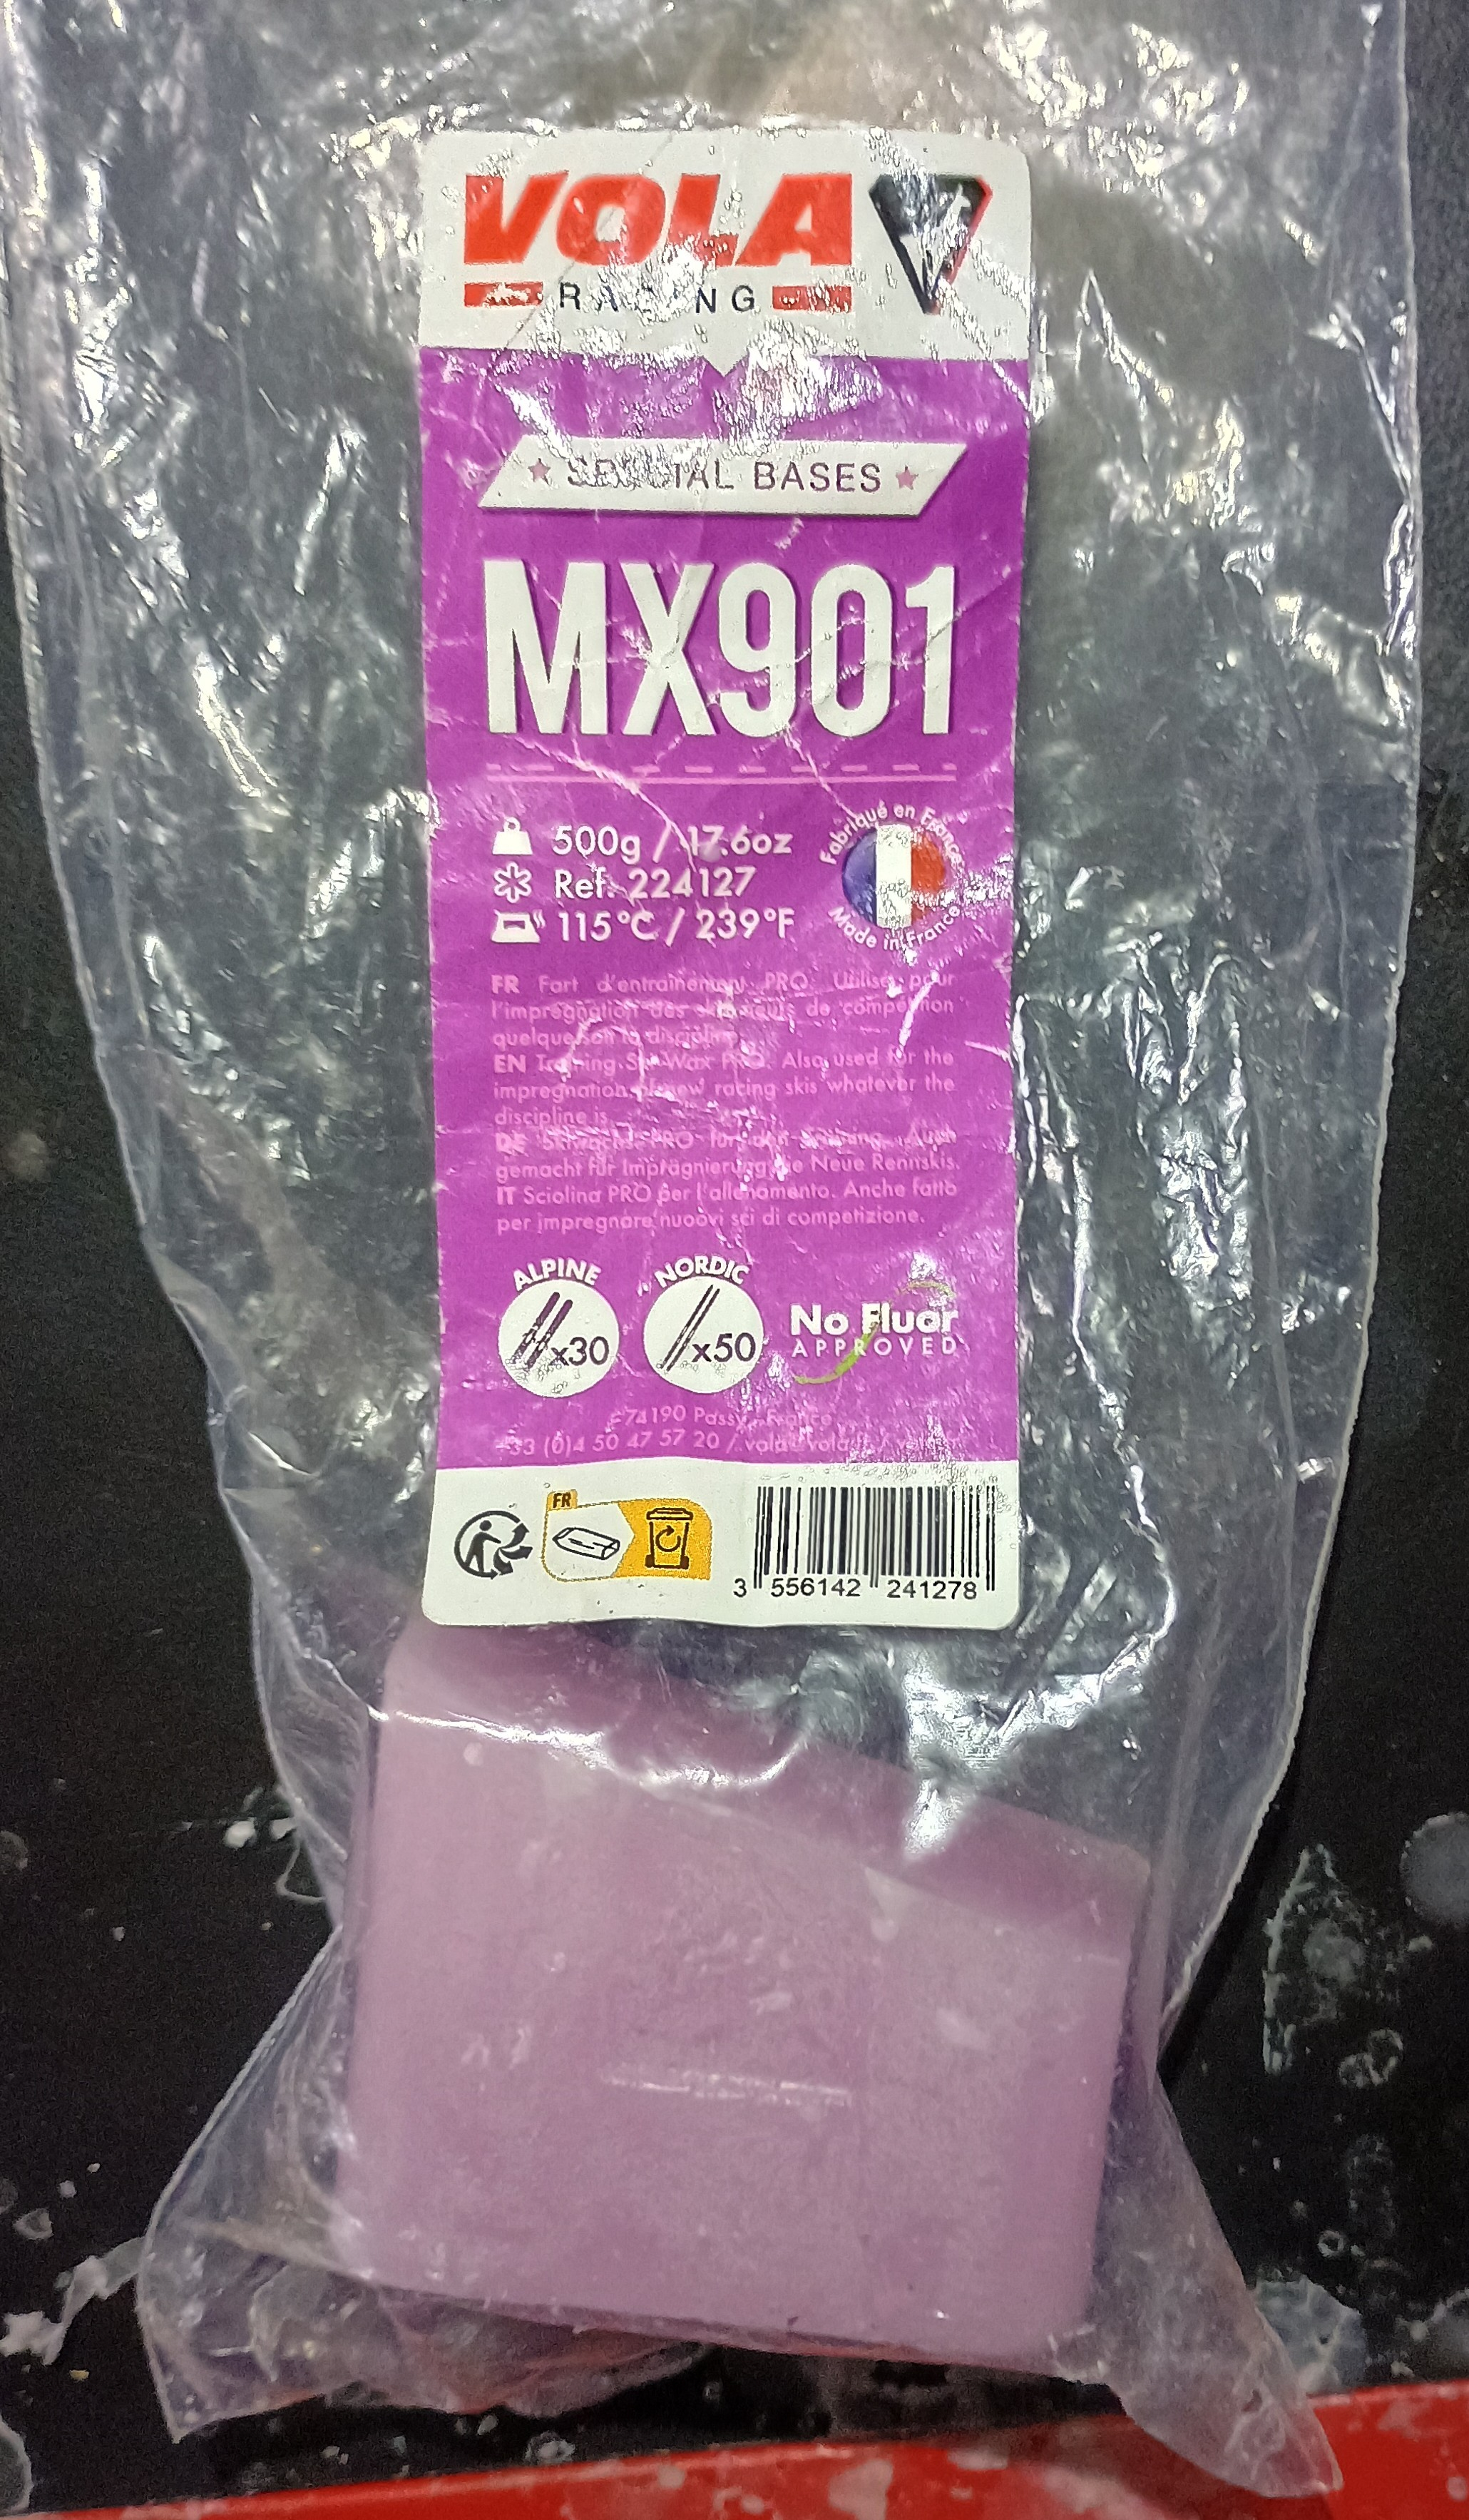
\includegraphics[width=0.9\linewidth]{Exp_1_St.Moritz/Wax_Vola_Laus.jpg}
        \captionof{figure}{Le fart utilisé pour toutes les expériences}
        \label{Vola_MX}
\end{minipage}
\begin{minipage}{0.3\textwidth}
    Ainsi, j'ai choisi une paire de skis skating (c'est le style ou il faut pousser sur le côté avec les jambes, il n'y a donc pas de zone croche)en très bon état (Fischer helium skate 100) qui est fait pour des conditions universelles. Ensuite, le ski doit avoir les mêmes propriétés du début jusqu'à la fin, il lui faut donc un fart qui tient longtemps sous la semelle et ne se dégrade pas trop vite. J'ai donc appliqué un fart qui n'est vu comme le "meilleur", mais comme un fart de base (les farts de base sont ceux qu'on applique sous le fart "performant" en compétition), qui a ces propriétés de tenir longtemps. Ce fart, le Vola MX901, a en plus la propriété d'être un fart plutôt universel, donc qui va bien pour presque toute les conditions.
\end{minipage}
\begin{minipage}{0.29\textwidth}
    \begin{center}
        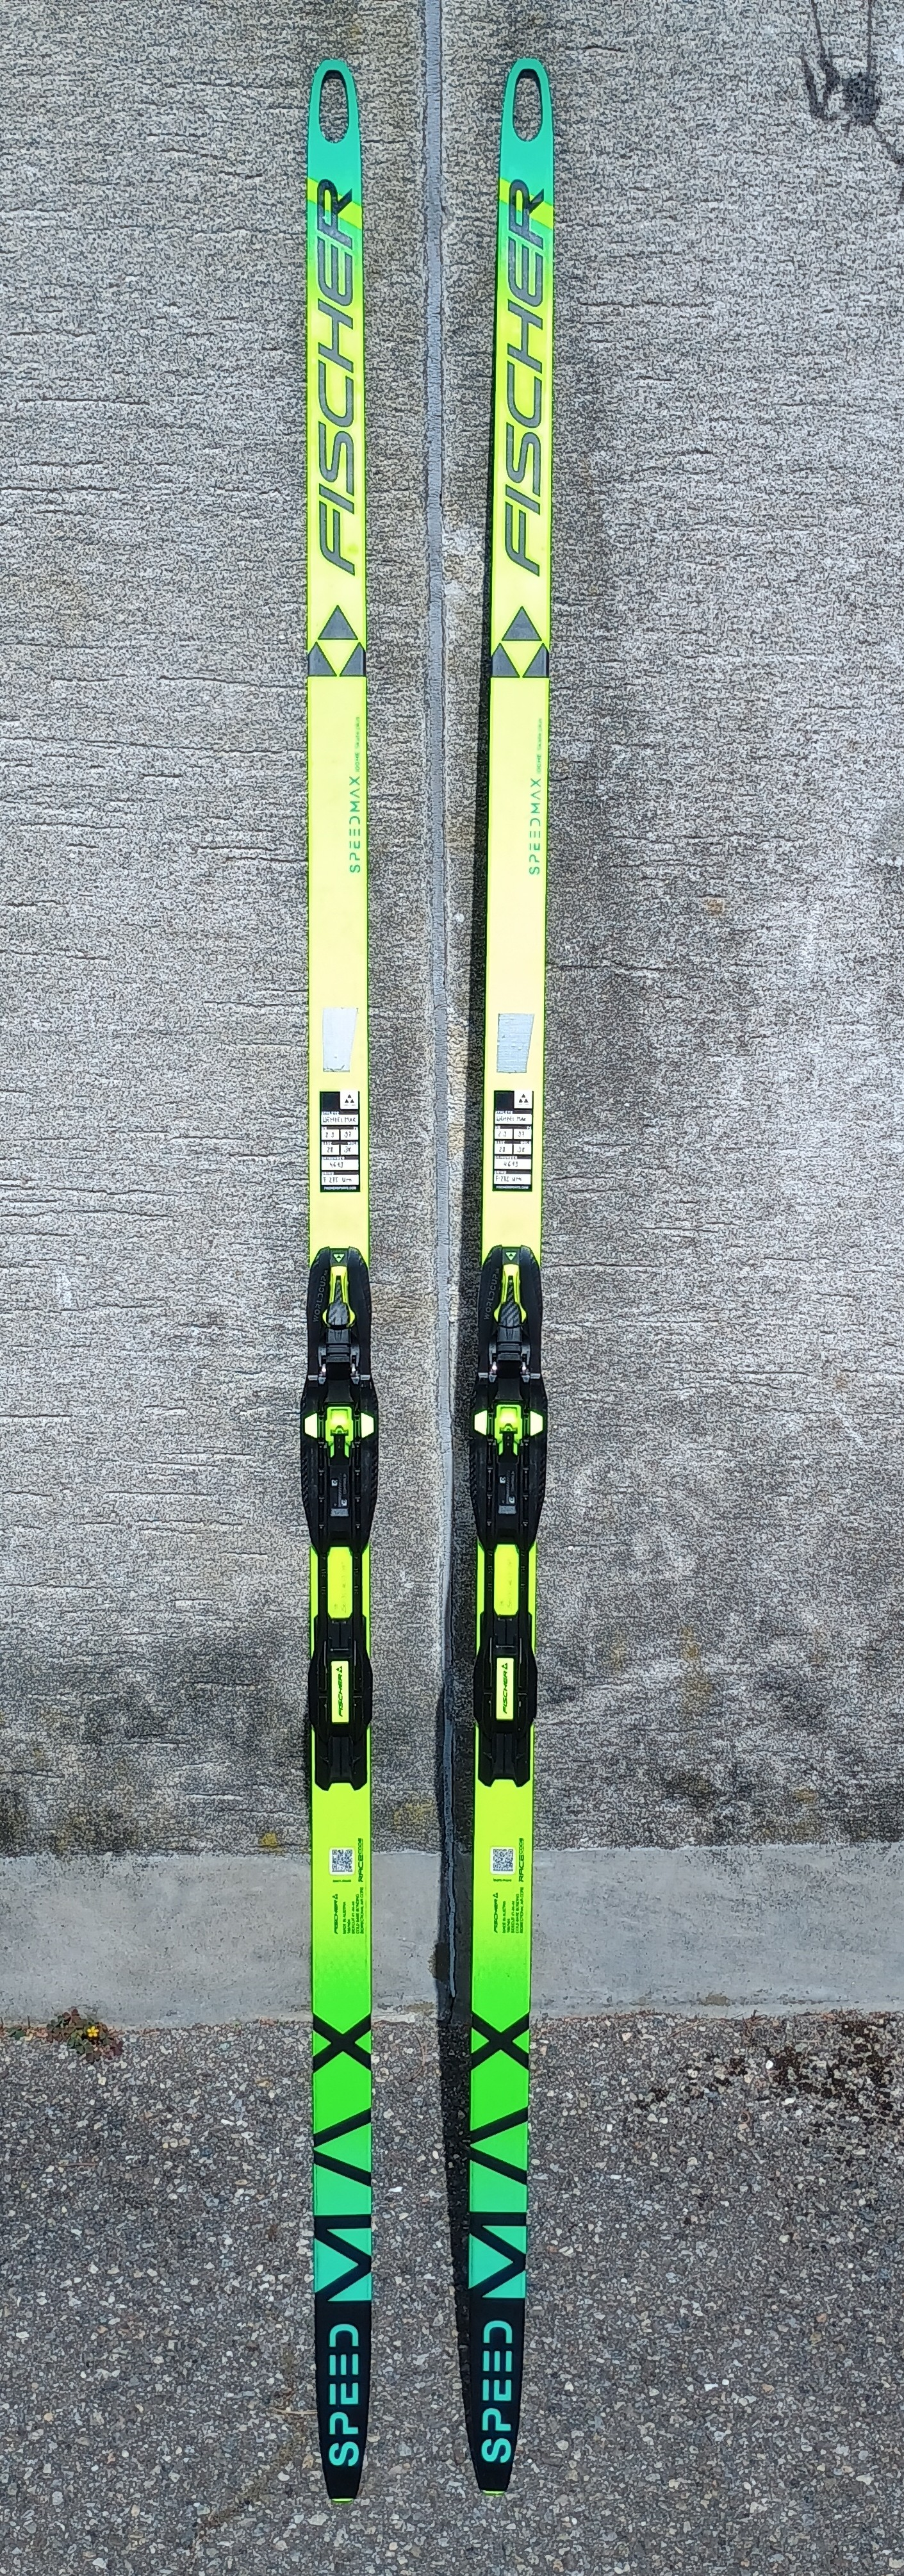
\includegraphics[width=0.8\linewidth]{Ski_surface_dry/Ski_Fischer_Laus.jpg}
        \captionof{figure}{Le ski utilisé pour les 2 premières expériences}
        \label{Fischer_Helium-skate}
    \end{center}
\end{minipage}

\vspace{0.5cm}

Le prochain paramètre est celui de la position du skieur. En effet, la position du skieur va être le chouss, pour simuler au mieux les descentes en competition. Même si cette position est utilisée par tout skieur, il faut quand même préciser 2-3 détails:

\begin{figure}[H]
    \centering
    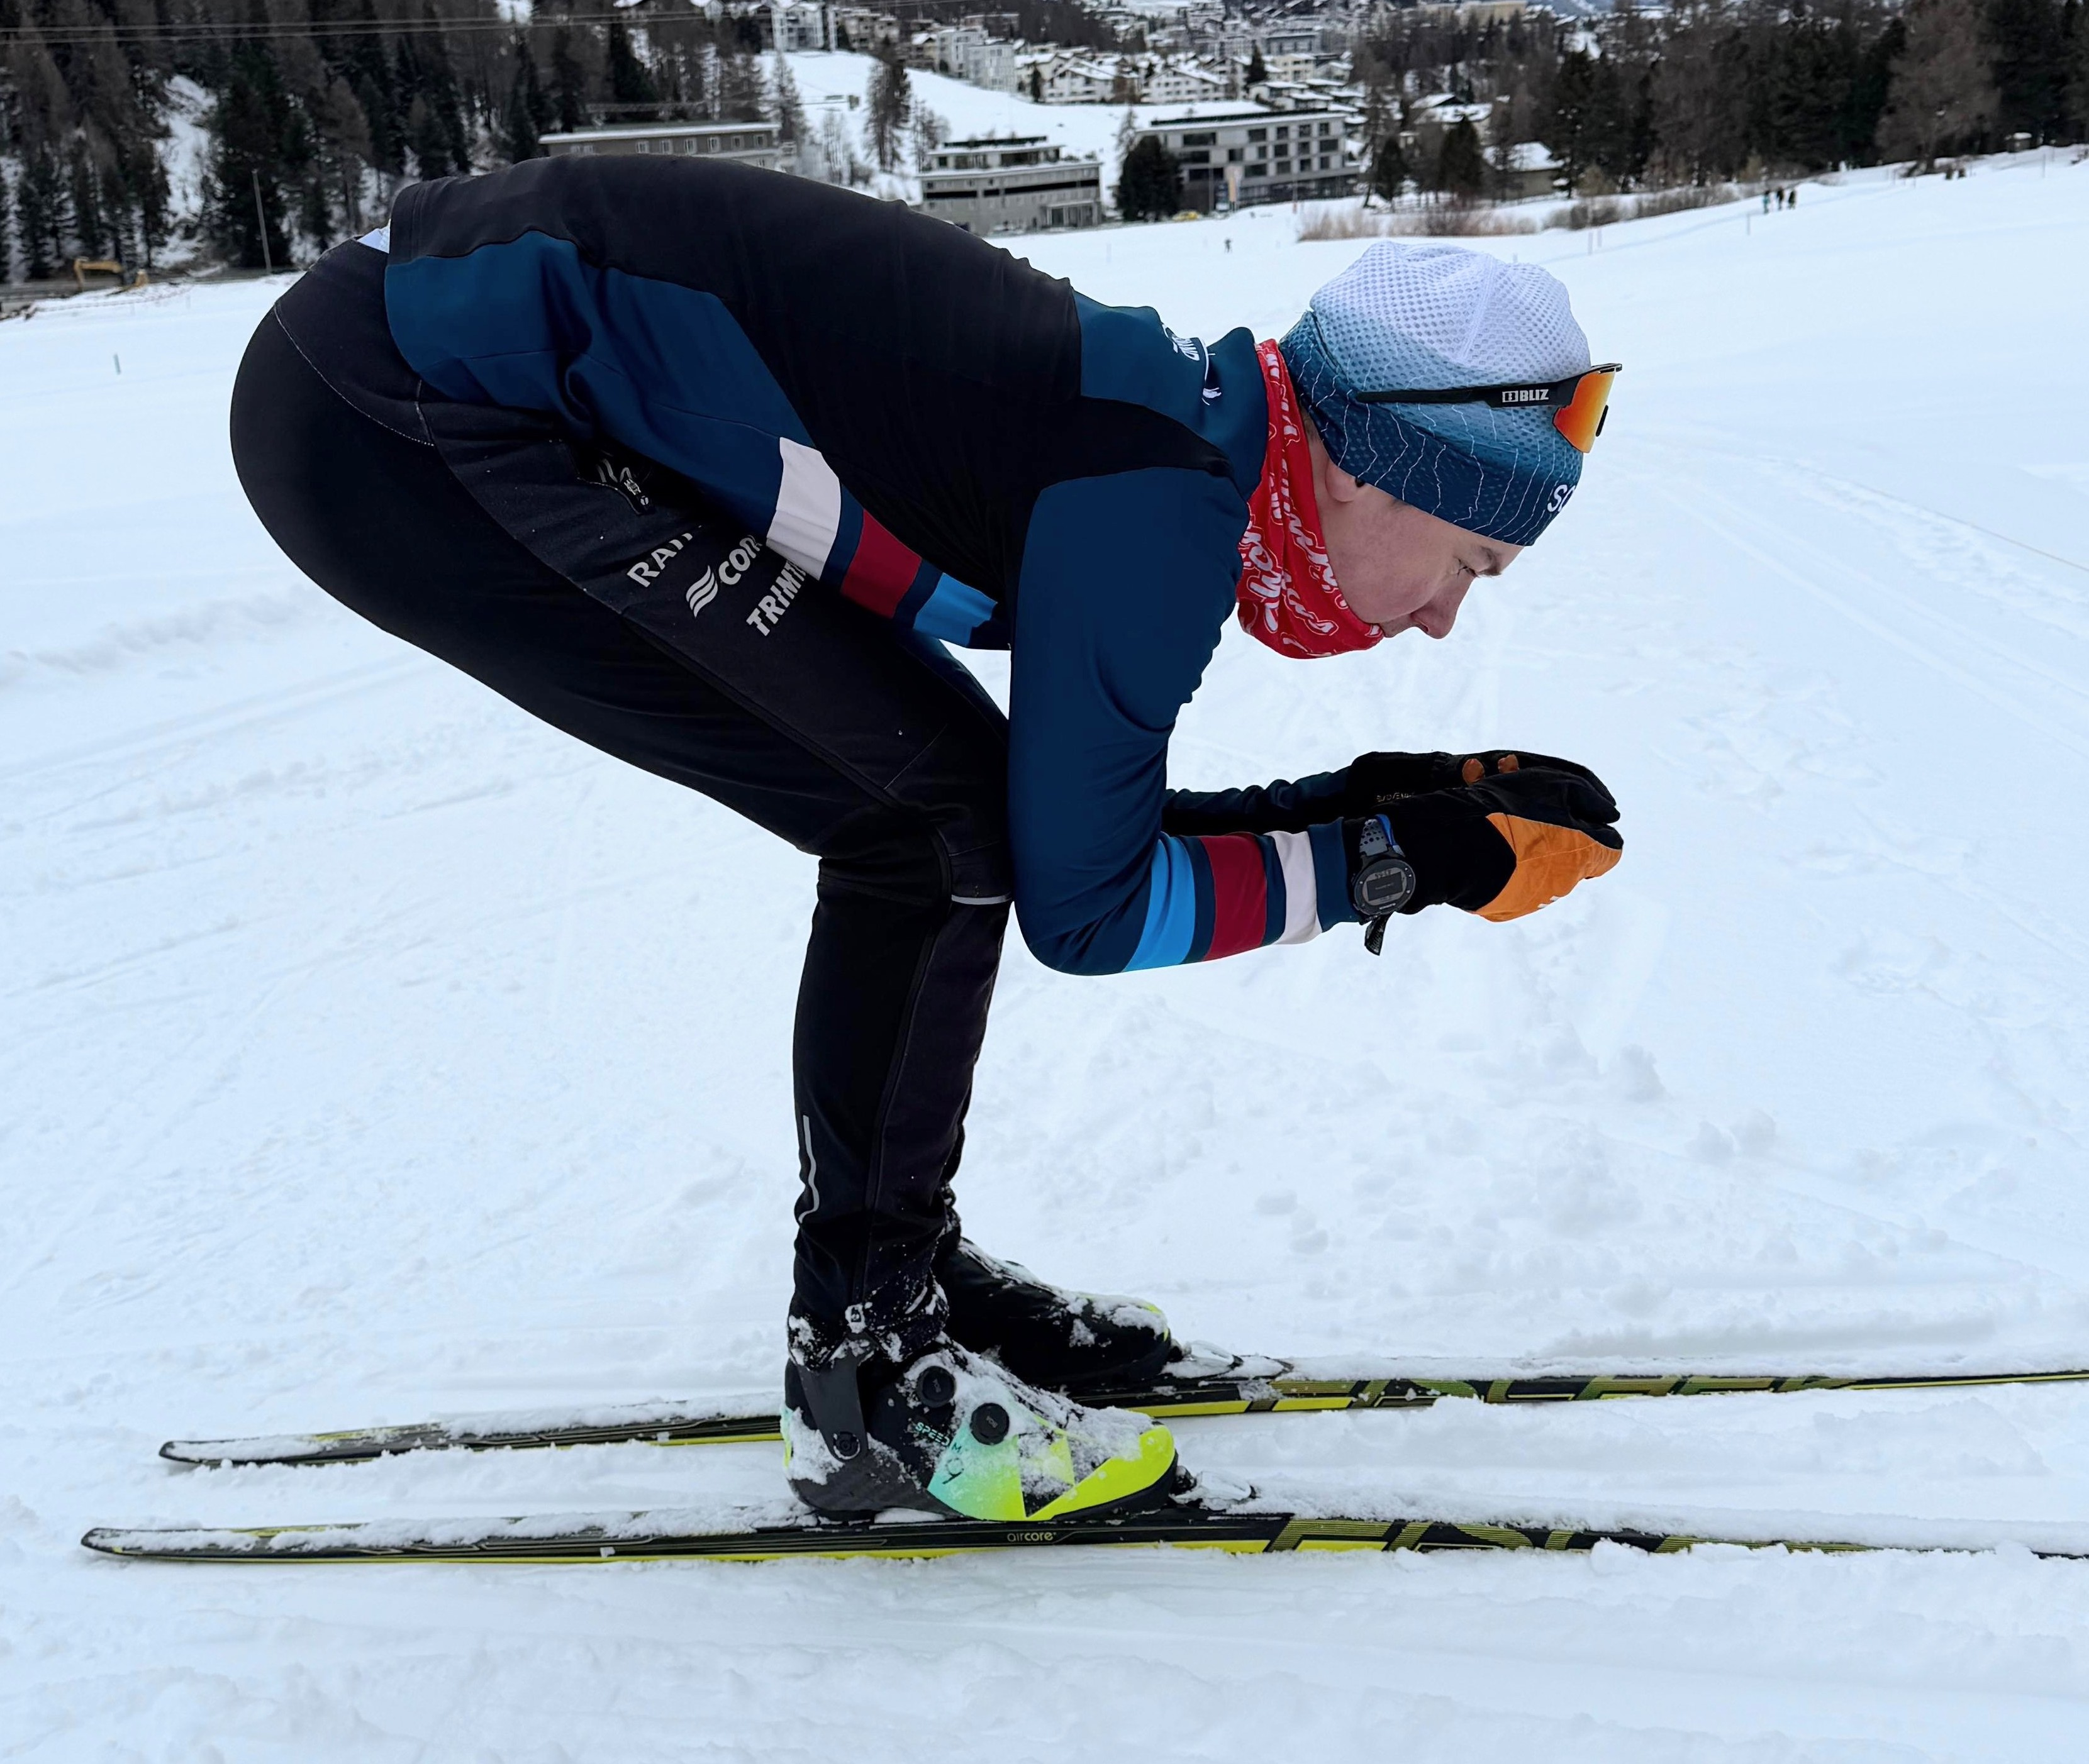
\includegraphics[width=0.75\linewidth]{Exp_1_St.Moritz/Mag_sit_position.jpg}
    \caption{La position de chouss: la tête et parallèle au sol, le regard vers le bas. Les hanches sont au moins à la même hauteur que la tête et les coudes sont si possible devant les genous, cela "verrouille" toute la position.}
    \label{Mag_chouss}
\end{figure}

Comme dit plus tôt, cette position varie quand même malgré ces instructions, car par exemple les personnes qui ne pratiquent pas le ski de fond  



\subsubsection{Déroulement (1)}

Il ne reste alors plus qu'une seule question: Comment chronométrer le temps dont le skieur a besoin pour atteindre l'arrivée? Nous nous sommes dit de le tenir pour l'instant au plus simple, alors nous avons imaginé le système  en 3 parties suivant: 

\begin{enumerate}

    \item La position de départ: le chronométreur est debout à l'arrivée et lève le bras, avec son telephone dans la main qui fait office de chronomètre. Au départ, le skieur est prêt en position de chouss, avec les skis dans la trace de l'expérience, il ne bouge plus à partir de ce moment. Le skieur est tenu par une troisième personne derrière lui, qui place l'avant des fixations des skis exactement sur la ligne de départ, qui perpendiculaire à la piste et à la hauteur du bâton et tracée par nous-même. 
    \newline Il y a ici déjà $2$ sources d'erreur qui sont claires avant même la prise de mesures: les $2$ sont liés à l'erreur humaine. Il y a premièrement le chronométreur pour lequel il est pratiquement impossible d'enclencher le chronomètre toujours exactement au même moment, alors qu'il fait un autre mouvement de l'autre bras et deuxièmement le temps de réaction de la personne qui tient le skieur: la directive était qu'elle lâche le plus vite possible dès qu'elle voit le signal, mais cela diffère chez la personne elle-même et surtout entre les différentes personnes. C'est pour cela qu'on a essayé de toujours mettre la même personne à ce poste, ce qui n'était pas possible quand cette personne était sur les skis elle-même. 
    \begin{figure}[H]
        \centering
        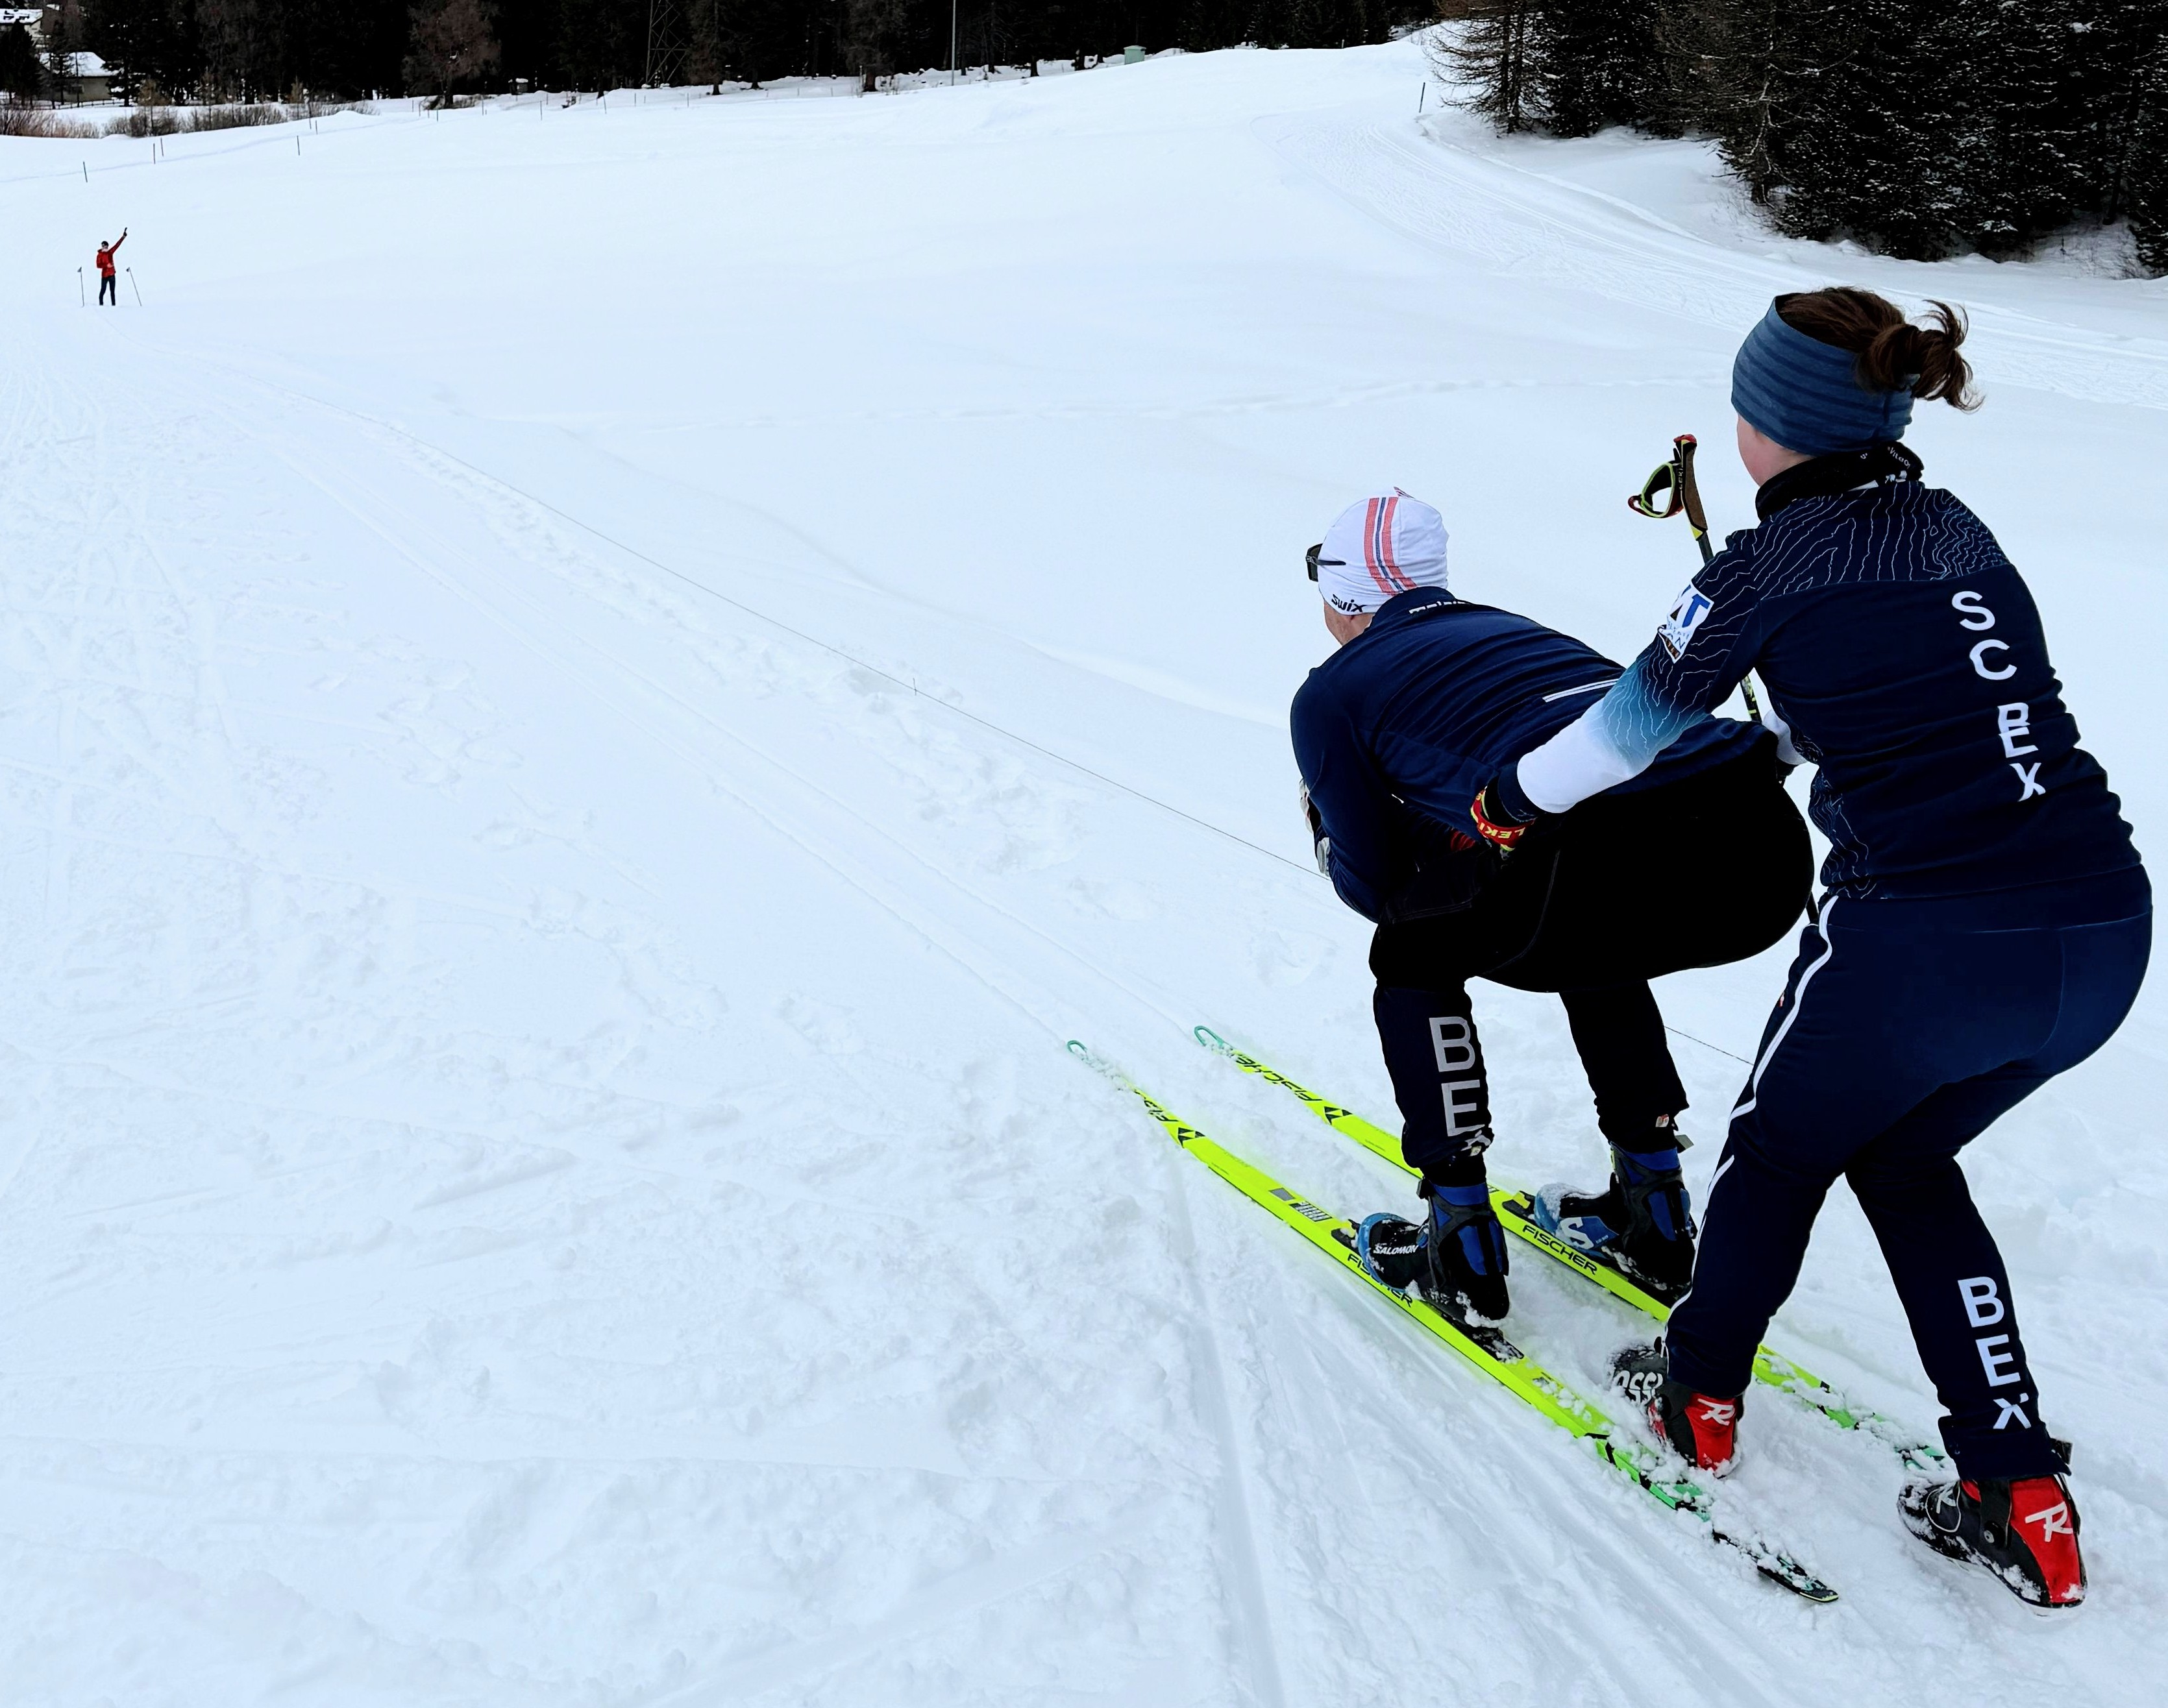
\includegraphics[width=0.8\linewidth]{Exp_1_St.Moritz/Elpa_start_St.Moritz(1).jpg}
        \caption{Photo qui illustre l'ensemble du positionnement au départ: À droite de la piste, un bâton qui marque le départ et, en-bas, un bâton qui marque l'arrivée avec le chronométreur à côté et la corde de 60m tendue entre les deux bâtons. Sur la piste, la personne derrière le skieur qui est attentive au signal du chronométreur et, devant elle, le skieur, avec les skis dans la trace faite maison, qui reste dans cette position pour le reste de la descente}
        \label{exp-1_global_start}
    \end{figure}

    \item Le départ: le chronométreur baisse d'un mouvement vif le bras, ce qui est le signal de départ. En même temps, il enclenche le chronomètre avec son autre main. Dès que la personne qui tient le skieur voit le signal de départ du chronométreur, il lâche le skieur le plus vite que possible. Le skieur commence alors à glisser dans la trace sans rien faire sauf rester en chouss.   

    \item L'arrivée: Le skieur glisse donc dans la trace pendant que le chronomètre tourne. À l'arrivée, le chronométreur se prépare à arrêter le chronomètre en se plaçant perpendiculairement à la ligne d'arrivée et au bâton d'arrivée. Après, il observe la ligne et le skieur et arrête le chronomètre quand l'avant des fixations du ski passent l'arrivée. 
    \newline Il y a bien sûr ici encore une troisième source d'erreur qui est déjà evidente avant d'avoir prise les mesures, qui est encore une fois l'erreur humaine: il est totalement impossible pour le chronométreur d'arrêter le chronomètre à la milliseconde près.

    \begin{figure}[H]
        \centering
         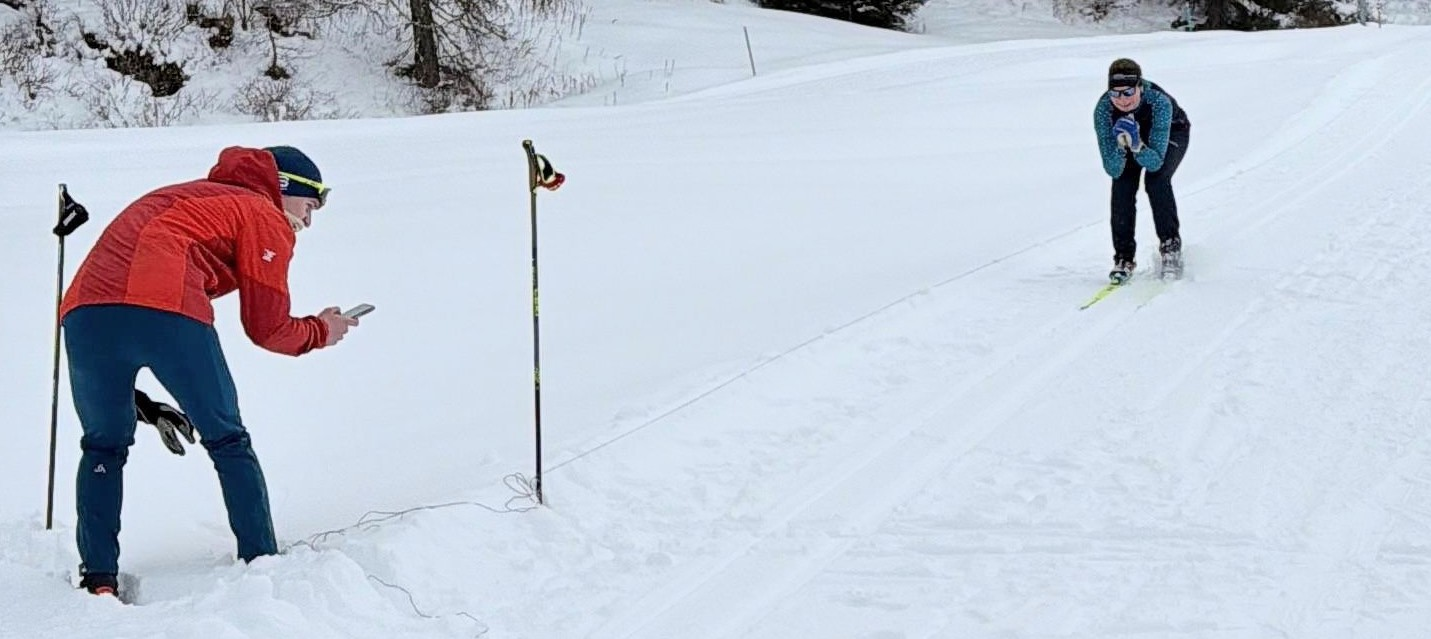
\includegraphics[width=0.9\linewidth]{Exp_1_St.Moritz/Tris_ma_finish_St.Mo.jpg}
        \caption{On voit l'arrivée: le chronométreur est attentif au skieur, il est prêt à arrêter le chronomètre.}      
        \label{St.Mo-finish_bad_position}
    \end{figure}
\end{enumerate}

On peut aussi représenter l'expérience sous forme de schéma: 

\begin{center}
    \begin{tikzpicture}
    \draw (1,0) -- (6,3);
    \draw (6,3) -- (6,0);
    \draw (6,0) -- (1,0);
    \draw (3.8,2) circle (0.25);

    \draw node at (0.8,0) {$A$};
    \draw node at (6.2,3.1) {$B$};
    \draw node at (6.2,0) {$C$};
    \draw node at (1.7,1) {$60[m]$};
    \draw node at (5.5,1) {$8[m]$};
    \end{tikzpicture}
\end{center}
\begin{itemize}
    \item où:
    \begin{itemize}
        \item $A$ est l'arrivée du skieur et la position du chronométreur
        \item $B$ est le départ du skieur, le temps qu'est donc mesuré est celui dont le skieur a besoin pour parvenir de $B$ à $A$
        \item $60[m]$ est la distance entre le départ et l'arrivée, qui ne nous sert seulement à dire si cette expérience-là était plutôt de distance courte ou longue par rapport au autres
        \item $8[m]$ est la dénivélation négative entre le départ et l'arrivée, mesurée avec les différents altimètres de nos montres. En effet cette dénivélation n'est pas très précise mais elle aussi ne fait que nous donner un ordre de grandeur de la pente par exemple qui est, par le théorème de Pythagore: $\frac{8}{\sqrt{60^2-8^2}}*100 \approx 13.45\%$
    \end{itemize}
\end{itemize}

Ensuite, pour pouvoir constater des différences de vitesses ou pas entre les différentes masses, il faut bien sûr différents skieurs avec différentes masses. Pour cela, j'ai pris pour ma première expérience ma famille dont la fourchette de masse passe de $45[kg]$ à $76[kg]$. Nous étions $5$ personnes et avons essayé de ne pas concevoir l'ordre de passage selon un certain critère, mais de le garder d'une certaine manière aléatoire. Pour obtenir une moyenne de temps, chaque personne a fait 3 passages.

\subsubsection{Résultats et analyse (1)}

Voici donc les résultats:

\begin{center}
\resizebox{1\textwidth}{!}{
    \begin{tabular}{|l|l|r|r|r|r|r|r|}
        \hline
        Personne   & $m [kg]$ & $t_1 [s]$ & $t_2 [s]$ & $t_3 [s]$ & $t_{moy} [s]$ & Ince. abs. [$s$] & Ince. prop. [\%]\\ \hline
        A   & 65 & 14.66 & 14.65 & 14.10 & 14.47 & 0.37 & 2.55701\\ \hline
        B   & 45 & 14.33 & 14.36 & 14.33 & 14.34 & 0.02 & 0.13947\\ \hline
        C   & 75 & 13.93 & 13.71 & 13.91 & 13.85 & 0.14 & 1.01083\\ \hline
        D   & 76 & 13.70 & 13.65 & 13.68 & 13.67 & 0.02667 & 0.19498\\ \hline
        E   & 74 & 13.75 & 13.46 & 13.45 & 13.55 & 0.19667 & 1.45106\\ \hline
        A   & 65 & 13.64 & 13.36 & 13.28 & 13.43 & 0.21333 & 1.58888\\ \hline
    \end{tabular}
    }
\end{center}
\begin{itemize}
    \item où
    \begin{itemize}
        \item La colonne "Personne" indique de quelle personne il s'agit, on notera que la personne $A$ y figure $2$ fois.
        \item $m$ est la masse de la personne
        \item $t_1$, $t_2$ et $t_3$ sont les temps de passages 1, 2 et 3 des skieurs
        \item $t_moy$ est le temps moyen des $3$ passages
        \item "Ince. abs." est l'incertitude absolue du temps moyen, il s'agit de la valeur absolue de la difference entre le temps moyen et le temps qui diffère le plus de celui là.
        \item "Ince. prop." est l'incertitude proportionnelle au temps moyen. Elle est calculée en divisant l'incertitude absolue avec le temps moyen et en multipliant tout cela par 100.
    \end{itemize}
\end{itemize}

Une première chose qu'on peut remarquer est que l'incertitude proportionnelle entre les temps de passages de chaque skieur est de moins de $2.6\%$, ce qui veut dire que les temps de passages d'un skieur étaient encore assez similaires entre eux. Cela implique aussi que les sources d'erreur dues à l'erreur humaine sont très probablement présentes, mais ne sont pas autant significatives que ce que je pensait avant de voir les mesures. 

\vspace{0.3cm}

Il y a cependant un autre effet qui a biaisé les mesures. Pour le remarquer, il faut savoir que le tableau est classé en ordre chronologique des mesures. L'ordre des lignes correspond donc à l'ordre de passage des skieurs. En effet, on remarque que les temps moyens ne font que se réduire, complètement indépendamment de la masse du skieur. Il a donc dû y avoir quelque chose qui augmentait l'accélération et la vitesse après chaque passage. Nous avons déjà observé ce phénomène pendant l'expérience et avons donc décidé que le premier skieur refait $3$ passages après tout-le-monde pour vérifier notre hypothèse et c'est pour cela que la personne $A$ est représentée $2$ fois dans le tableau. On peut voir que, en effet, le temps moyen de la personne $A$ se réduit de $1.03[s]$. Cela représente une réduction de $\sim 7.77\%$, ce qui est quand même énorme. 
\newline On peut y ajouter que c'est effet a complètement caché la potentielle influence qu'à la masse sur la vitesse. Le graphique suivant est utile pour visualiser tout ce qui est dit ci-dessus.



\begin{center}
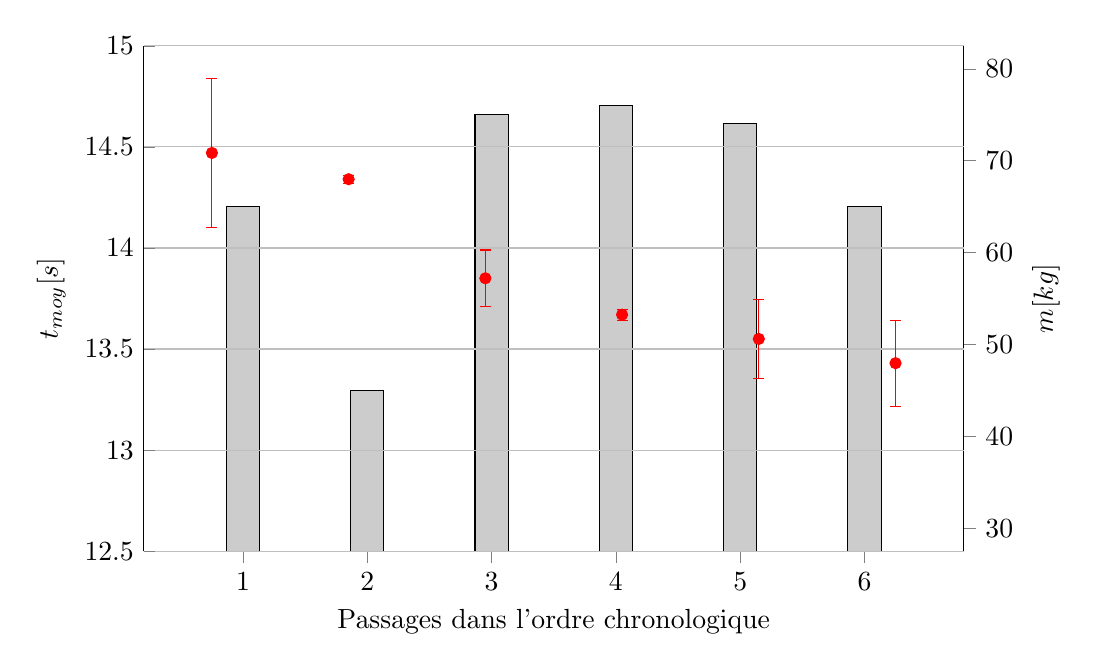
\begin{tikzpicture}
\begin{axis}[
    width=12cm,
    height=8cm,
    xmin=0.5, xmax=6.5,
    ymin=30, ymax=80,
    xtick={1,2,3,4,5,6},
    axis y line*=right,
    axis x line*=bottom,
    xlabel={Passages dans l'ordre chronologique},
    xbar,
    ylabel={$m [kg]$},
    ybar,
    bar width=12pt,
    enlargelimits=0.05,
]

\addplot[
    fill=gray!40,
    draw=black
]
coordinates {
    (1,65)
    (2,45)
    (3,75)
    (4,76)
    (5,74)
    (6,65)
};

\end{axis}

\begin{axis}[
    width=12cm,
    height=8cm,
    xmin=0.5, xmax=6.5,
    ymin=12.5, ymax=15,
    xtick=\empty,
    axis y line*=left,
    axis x line=none,
    ylabel={$t_{moy} [s]$},
    grid=both,
]

\addplot[
    color=red,
    mark=*,
    only marks,
    error bars/.cd,
    y dir=both,
    y explicit,
]
coordinates {
    (1,14.47) +- (0,0.37)
    (2,14.34) +- (0,0.02)
    (3,13.85) +- (0,0.14)
    (4,13.67) +- (0,0.02667)
    (5,13.55) +- (0,0.19667)
    (6,13.43) +- (0,0.21333)
};
\end{axis}
\end{tikzpicture}  % code de ChatGPT end
\captionof{figure}{Graphique qui représente les temps moyens de passages en fonction de l'ordre de passage avec les points rouges et le poids correspondant des skieurs représentés par les barres grises. On peut clairement y voir que les temps moyens se réduisent au fil des passages, tandis que la masse n'a pas d'influence.}
\end{center}

 Mais alors, comment cet effet se produit-il?

\begin{minipage}{0.55\textwidth}
    Au fait, c'est nous sommes presque sûr que c'est dû au fait que j'ai tracé la trace moi-même. Comme mentionné dans la partie sur la théorie réaliste, un ski fait fondre la neige en-dessous de lui, et c'est ce qui le fait avancer. En effet, après que le skieur soi passé, une partie de cette eau fondue va rester sur la neige et surtout se resolidifier, elle va devenir de la glace. Cet effet est très connu en ski de fond et il se produit, comme dans notre expérience, surtout sur de la nouvelle neige. On arrive souvent même à le voir par le reflet du ciel, comme dans la photo ci-contre, et on appelle une telle trace une "trace lustrée". En effet, les forces de frottements entre le ski et la glace sont moins importants qu'entre le ski et la neige. À chaque passage donc, de plus-en-plus de glace s'accumule sur la surface de la neige et la trace devient de plus-en-plus rapide. 
    \newline Il y a cependant un moment où il y a tellement de glace que encore plus n'aura aucune influence, vu que la neige en-dessous ne touche même plus le ski. C'est pour cela que c'est le fait que nous avons fait l'expérience dans une nouvelle trace qui a amené cet effet d'accélération. En effet, une trace formée par la machine est déjà plus dure de base et il y a plein de personnes qui y sont déjà passées. La trace est donc la principale source d'erreur de cette expérience
    
\end{minipage}
\begin{minipage}{0.45\textwidth}
    \begin{center}
        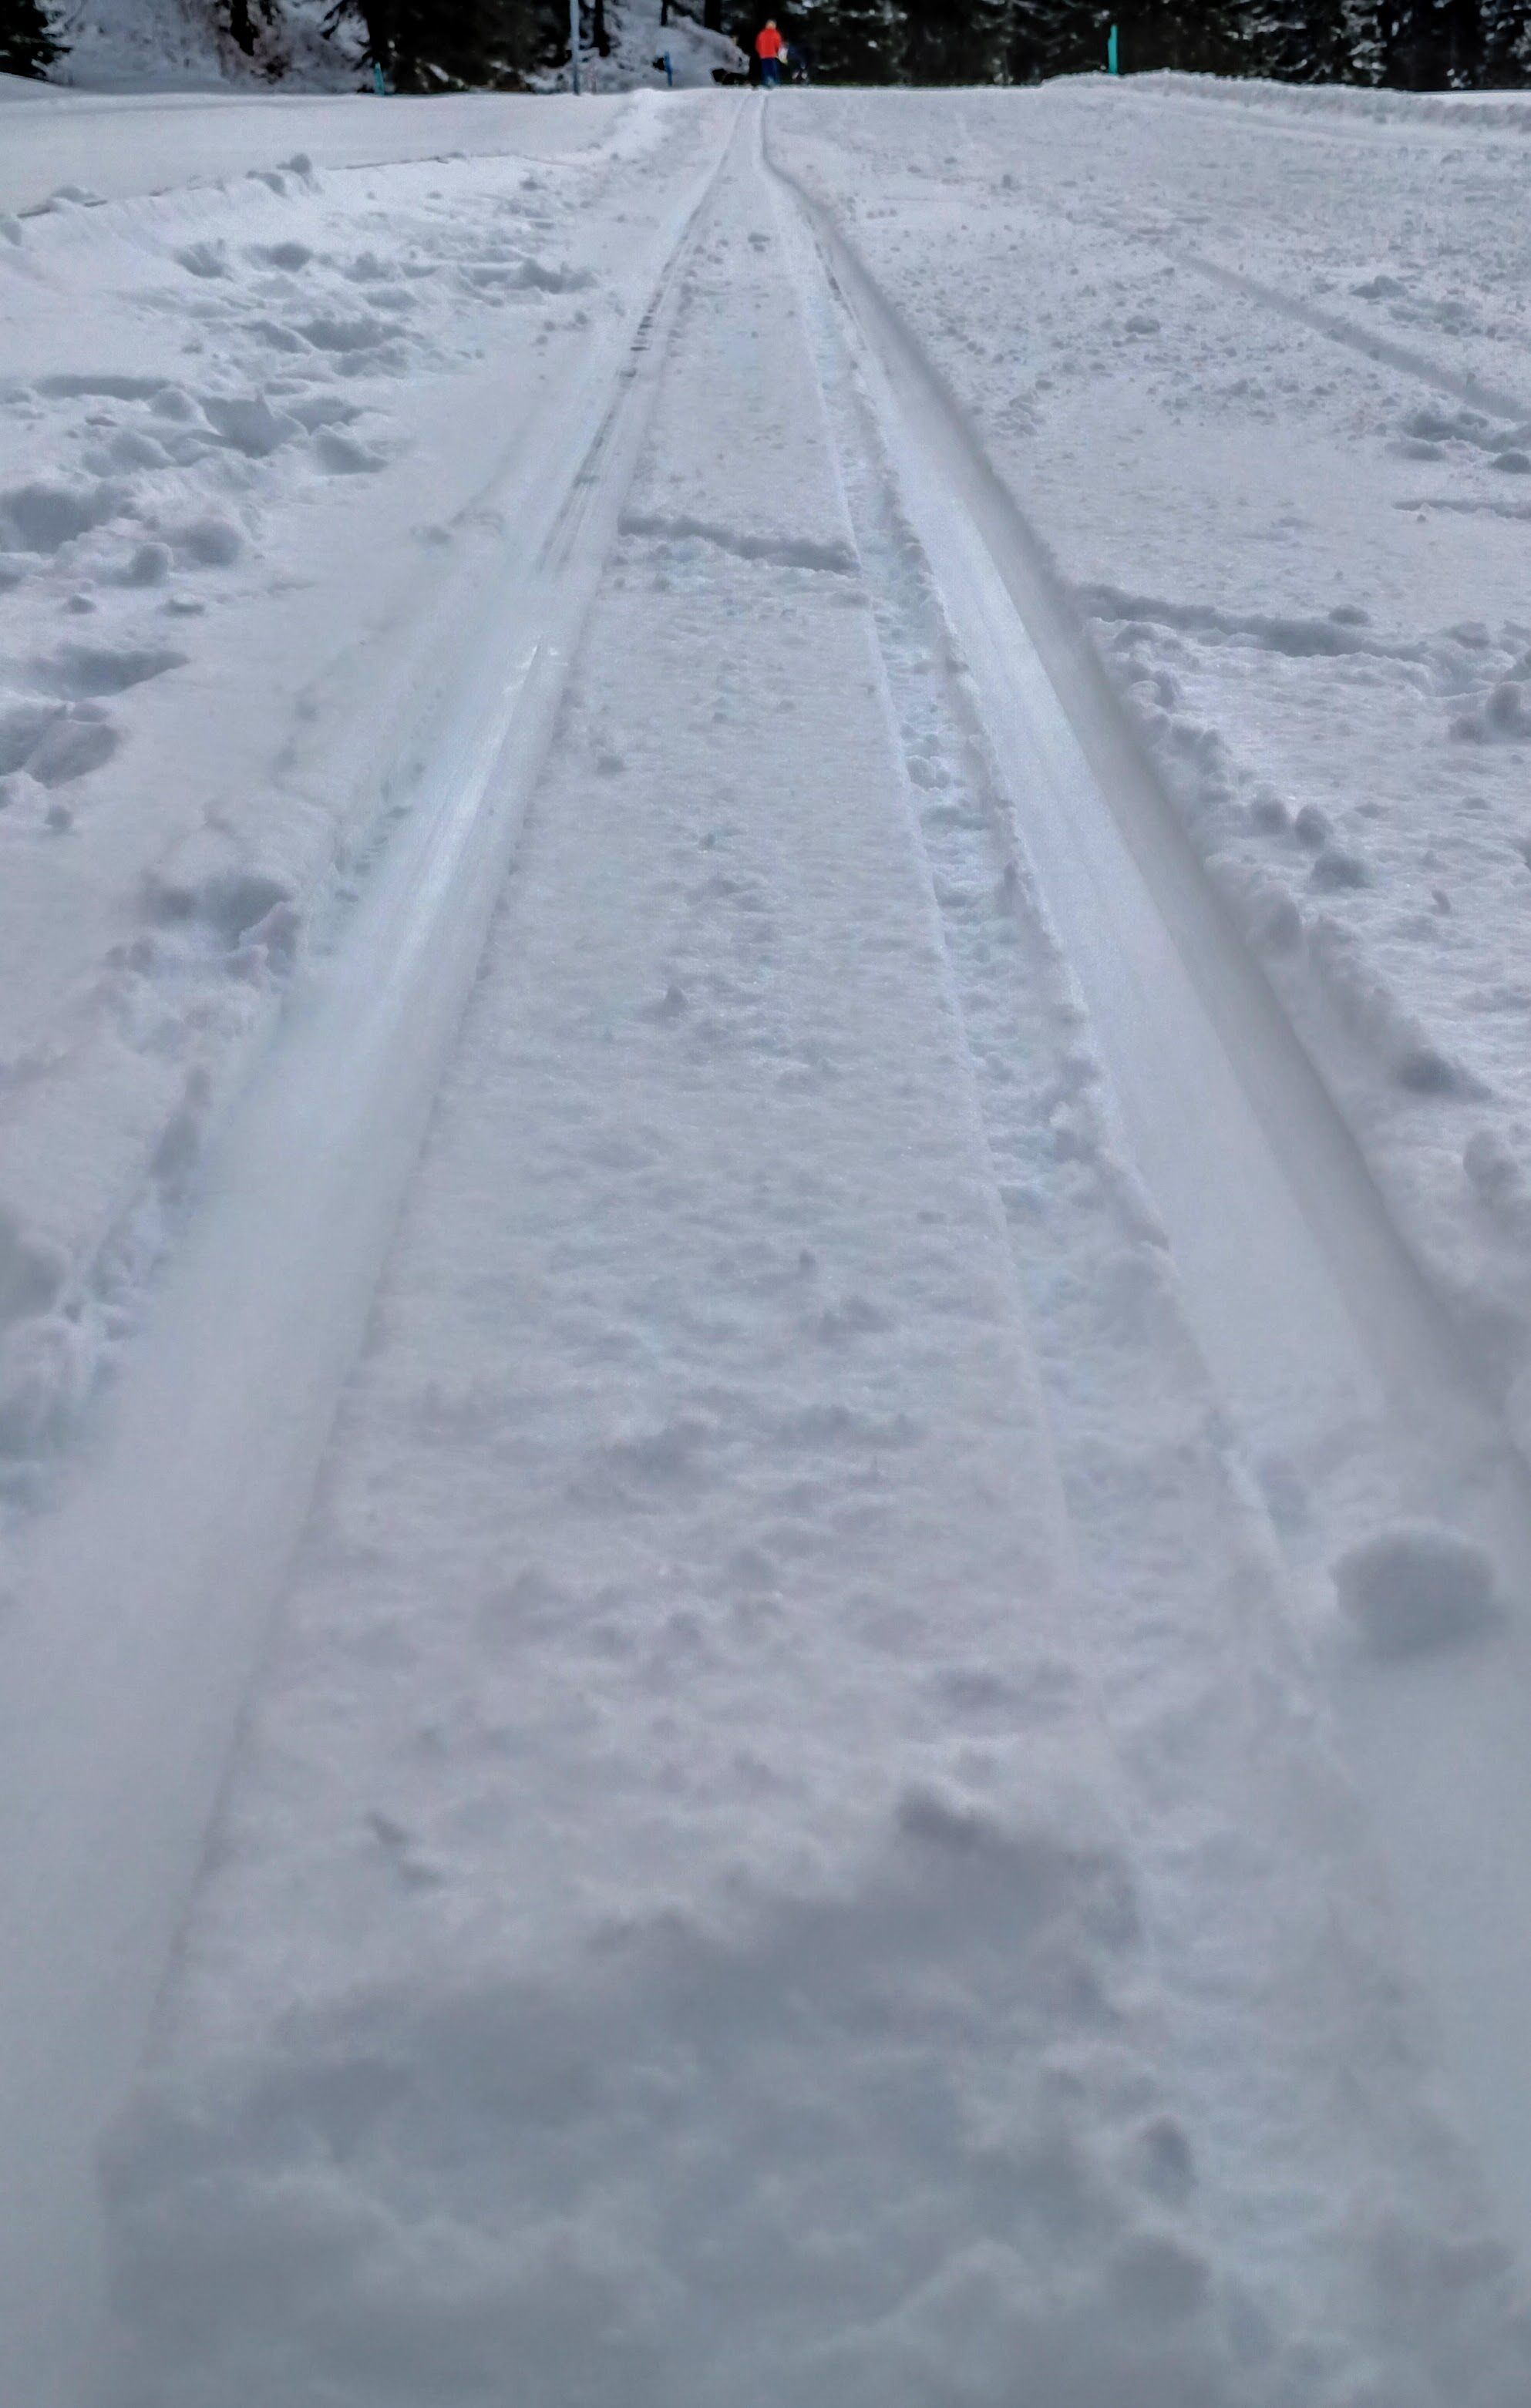
\includegraphics[width=0.85\textwidth]{Exp_1_St.Moritz/Track_icy.jpg}
        \captionof{figure}{La trace de l'expérience lustrée après tous les passages}
        \label{ICE_track}
    \end{center}
\end{minipage}

Une question que l'on m'a aussi posé quand j'ai parlé de cette expérience est: comment se fait-il que les temps des 3 passages d'un skieur ne diffèrent pas beaucoup alors que les différences entre les temps moyens entre les skieurs sont assez significatives?
\newline Tout d'abord, il faudrait peut-être dire que les $7.77\%$ ne sont pas arrivés d'un skieur à l'autre, mais il y a bien eu $5$ skieurs entre. En effet, la réduction maximale de temps moyen entre 2 skieurs est celle entre le 2ème et 3ème skieur, donc entre les personnes B et C: elle est de $\sim 3.42\%$, ce qui n'est plus très loin de l'incertitude maximale trouvée sur les 3 passages d'un seul skieur.. $\sim 2.6\%$ 
\newline Il y a peut-être aussi la météo et le temps entre les passages qui y a joué un rôle. Comme nous avons fait l'expérience en fin d'après-midi, il a très légèrement fait plus froid, malgré les nuages. Cela a potentiellement encore accéléré la piste, et la arrive le temps entre les passages. En effet, un skieur qui doit refaire un passage ne doit seulement remonter et se remettre en position pour repartir alors que quand il faut changer de skieur, il faut changer de skis, et donner un dernier briefing sur la position avant qu'il puisse se mettre en position. Cet aspect a cependant à mon avis un rôle très très minimal en tant que source d'erreur, car la baisse de température était minimale.

\subsubsection{Sources d'erreurs à améliorer pour la prochaine expérience}

Pour les prochaines expériences, il faudra essayer d'éliminer ou en tout cas d'atténuer toutes les sources d'erreurs que nous avons eu dans cette expérience, afin d'obtenir des mesures "valides". Il y a eu:
\begin{enumerate}
    \item La trace qui s'est de plus-en plus lustrée: C'est la source d'erreur majeure de cette expérience, c'est sans doute la source d'erreur qui a rendu les résultats "invalides". Pour l'éviter dans ce qui suit, il faudra prendre nos mesures dans une trace préparée par la machine et faire plusieurs passages dedans avant de commencer l'expérience.
    
    \item Le chronométrage: Bien qu'elle n'ait pas été autant présente que prévue, cette source d'erreur a quand même le potentiel de biaiser les résultats. Il y avait premièrement le chronométreur qui devait appuyer sur les boutons à des moments exacts, et deuxièmement le temps de réaction de la personne qui tient le skieur. Pour donc pouvoir éliminer cette source qui se doit à l'erreur humaine, il faudra entièrement confier le chronométrage à des machines, comme par exemple un système qui enclenche et arrête automatiquement le chronomètre.

    \item La position du skieur: Je n'en ai pas tant parlé dans la discussion des résultats, mais c'est bien une source d'erreur à atténuer. Malgré les instructions sur la position que j'ai donné aux skieurs, il y encore pas mal de différence entre les skieurs, comme on peut le voir on comparant la photo \ref{St.Mo-finish_bad_position} et \ref{Mag_chouss}. Je n'aimerai cependant pas abandonner cette position, comme c'est la positon que nous adoptons dans les descentes en compétition. Nous allons donc introduire une deuxième position qui est beaucoup plus homogène parmi tout-le-monde. Cela nous permettra en plus de comparer ces positions. 
\end{enumerate}

\subsubsection{Conclusion expérience 1}
Pour donc résumer, cette expérience n'a pas encore fait ressortir quel rôle a la masse dans la vitesse d'un skieur de fond en descente. Cette expérience a donc surtout servi à faire ressortir les sources d'erreurs à éviter pour les prochaines expériences, où nous pourrons faire des mesures valides. 




\subsection{2ème expérience}

Nous avons fait la deuxième expérience à Pontresina, le 09.03.2026. Il y avait beaucoup de Soleil, mais nous l'avons faite tôt le matin et la neige était dure donc il n'y avait pas de changement de l'état de la piste.

\subsubsection{Préparation (2)}

Bien avant l'expérience, il fallait se demander comment faire le chronométrage sans qu'il y ait d'erreur humaine dedans. Nous sommes partis de l'idée qu'il y a sûrement un moyen de la faire avec $2$ téléphones et nous en avons en effet trouvé une application qui est faite pour cela. 
\newline Elle s'appelle \textit{Photo Finish}~\cite{photofinish} et a été spécialement conçue pour mesurer des temps dans le sport. Elle fonctionne de cette manière:
\vspace{0.3cm}

\begin{enumerate}
    \begin{minipage}{0.45\textwidth}
    \item On connecte $2$ téléphones ou plus dans l'application. Dans notre cas, c'est un téléphone pour le départ, et un téléphone pour l'arrivée. La connexion fonctionne par bluetooth. 
    
    \item Après, les caméras des $2$ téléphones servent de capteurs de passage. Il faut après placer le téléphone de sorte que la ligne verticale au milieu de la caméra, qui sert de ligne de départ et d'arrivée, s'aligne avec le départ et l'arrivée voulu. Pour faire cela, il faut bien sûr que le téléphone soit stable et "tienne debout" tout seul. Nous avons donc utilisé un trépied.
    
    \item Le déclenchage du chronomètre fonctionne par détection de mouvement: Dès que la caméra détecte un mouvement, elle prends pleins de photos à la suite jusqu'à ce qu'elle ne détecte plus aucun mouvement. L'algorithme va après tracer des lignes verticales au point le plus avancé de la personne. Une fois que l'algorithme a fait cela, il va garder les $2$ photos où les lignes verticales sont le plus proche de la ligne verticale du milieu (donc une juste avant et une juste après la ligne de départ), et effacer les autres. Il va après, avec ces $2$ photos donner une estimation au centième près de quand le skieur a passé la ligne. C'est le même fonctionnement pour arrêter le chronomètre à ligne d'arrivée.
    \end{minipage}
    \begin{minipage}{0.55\textwidth}
    \begin{center}
        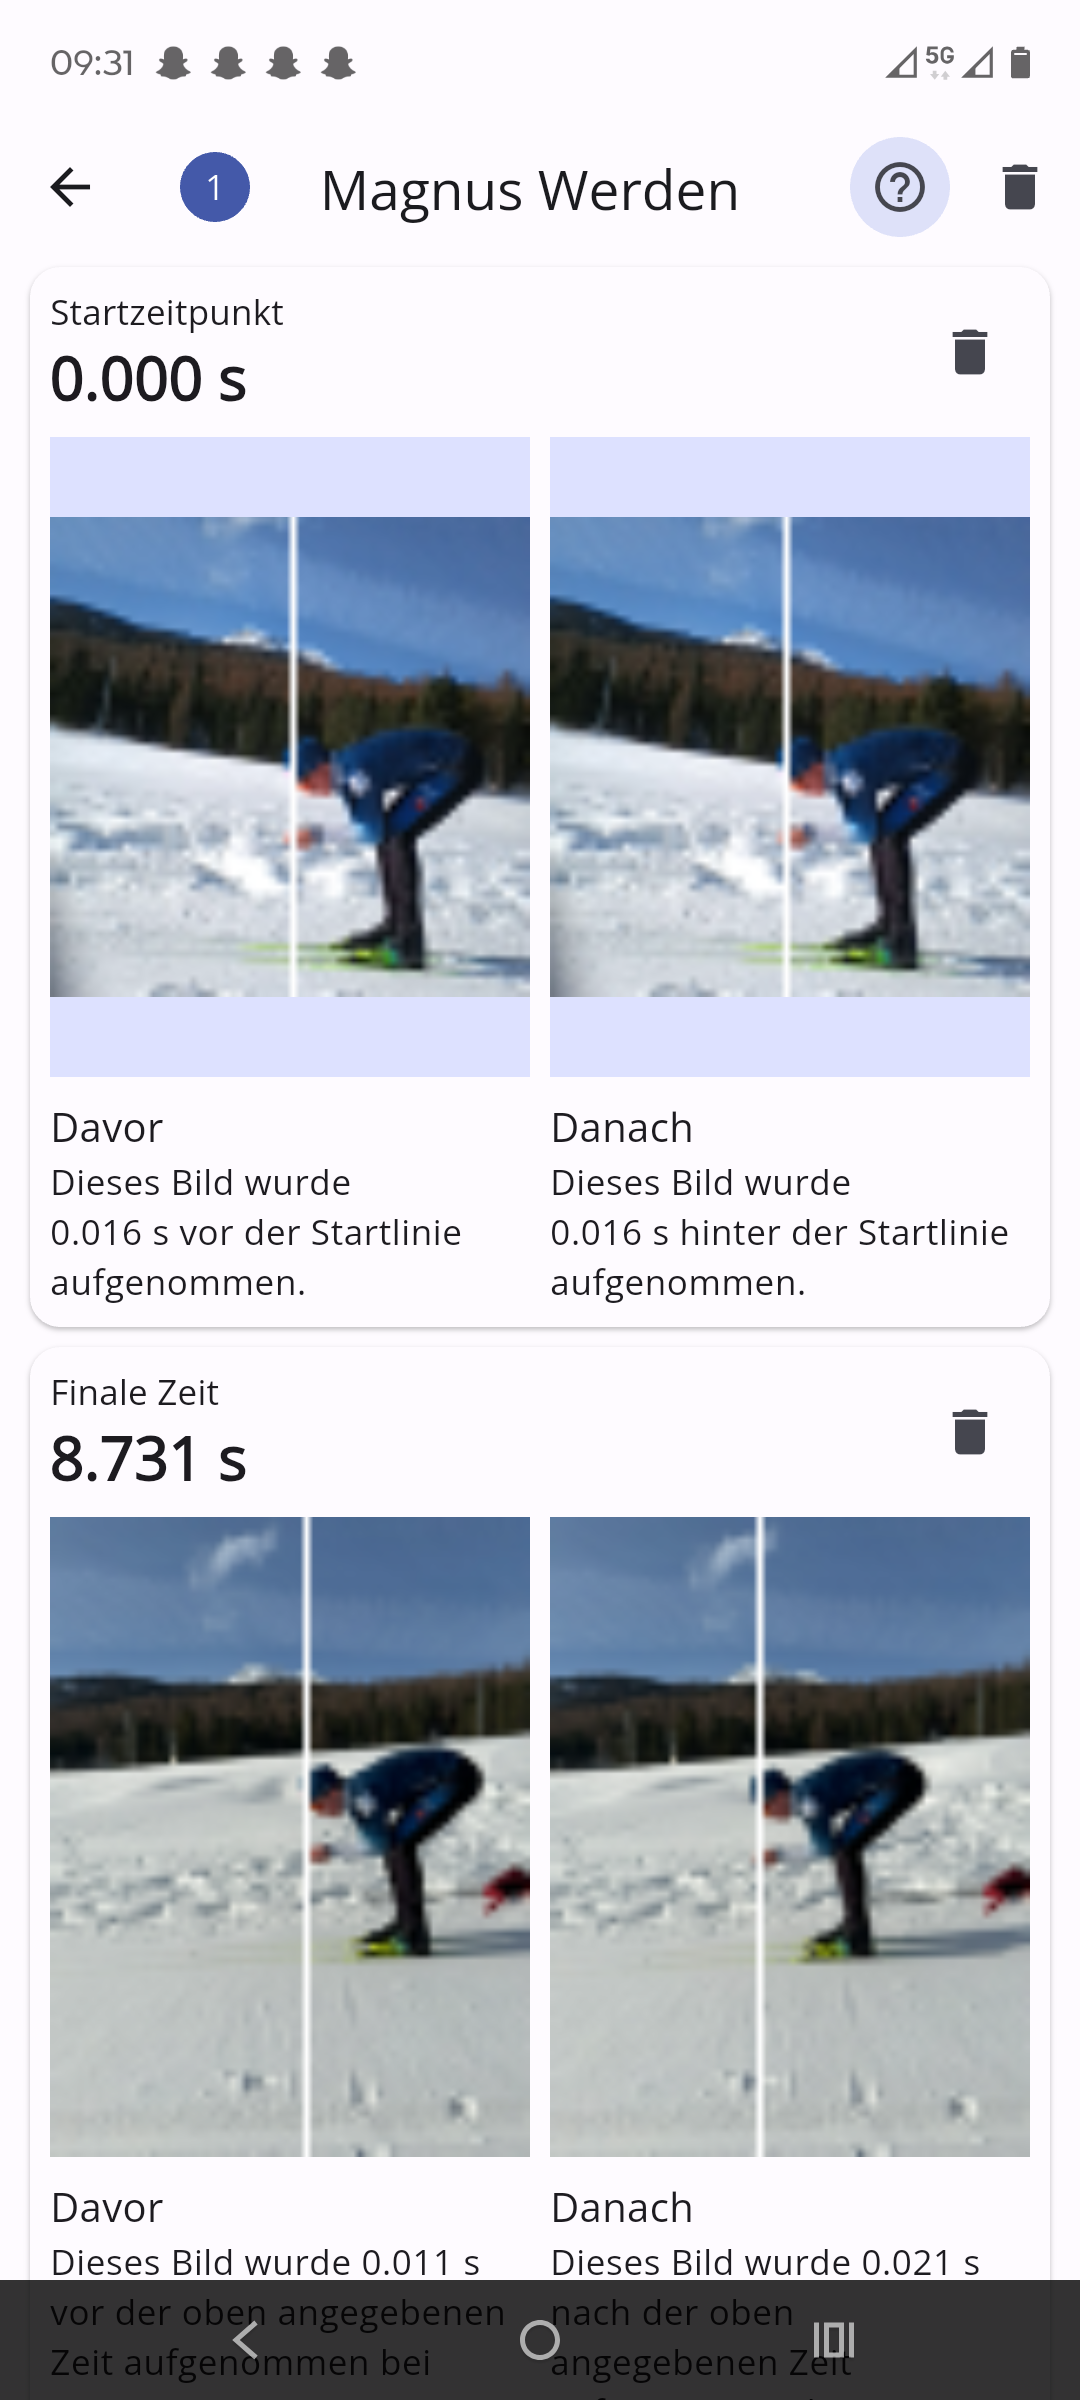
\includegraphics[width=0.7\textwidth]{Exp_2_Pontresina/Screen-photo-finish.png}
        \captionof{figure}{Fonctionnement de l'application: en-haut les $2$ photos du départ et en-bas celles de l'arrivée}
    \end{center}
\end{minipage}
\end{enumerate}
\vspace{0.5cm}

Ensuite, nous avons défini une nouvelle position. C'est tout simplement être debout:
\begin{figure}[H]
    \centering
    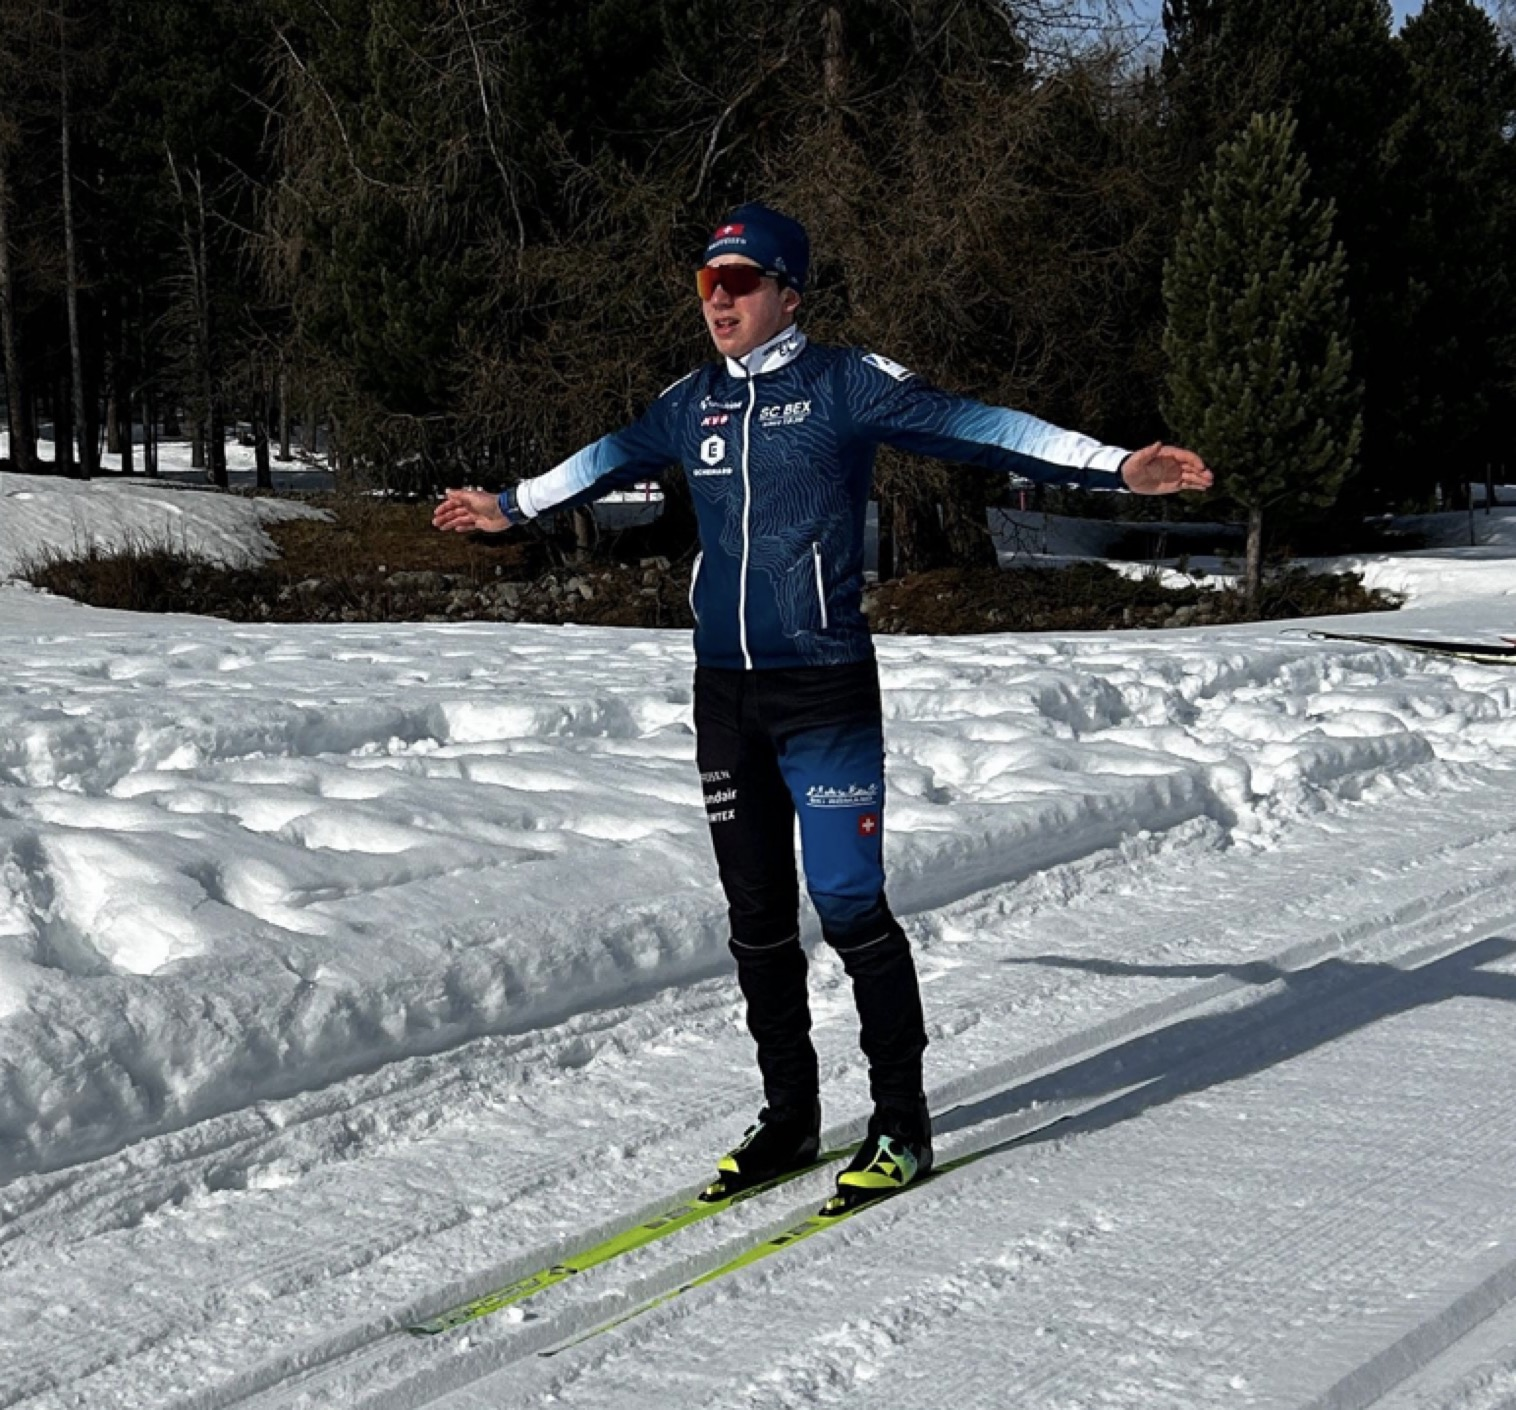
\includegraphics[width=0.75\linewidth]{Exp_2_Pontresina/pontre_stand_pos_2.jpg}
    \caption{La position debout: Les bras sont tendus et perpendiculaires au corps , les mains sont ouvertes. le regards est vers l'avant}
    \label{Standing_aura}
\end{figure}

Les avantages de cette postion sont:
\begin{enumerate}
    \item la simplicité: Contrairement au chouss, cette position est très égale chez tout-le-monde. C'est donc une source d'erreur atténuée.
    
    \item la surface séquante augmentée: Les forces de frottements de l'air seront plus grandes, ce qui a potentiellement comme effet que les différences de vitesse selon la masse ressortent plus. Additionellement, nous pourrons comparer les temps entre la position de chouss et la position debout. Cet aspect est potentiellement atténué par le fait que des skieurs plus lourds sont souvent aussi plus grands et plus large que des personnes plus légère. La differnece de taille est parfois aussi le cas chez des personnes de même poids, ce qui présente une petite source d'erreur.
    
    \item le chronométrage: Le système décrit plus haut est encore plus fiable sur cette position car le point le plus en avant est toujours le même. (selon les skieurs le point le plus en avant lors du chouss est la tête ou les mains, ce qui créé une légère source d'erreur lors du chronométrage) 
\end{enumerate}

Après, il a fallu trouver une trace dans laquelle faire cette expérience. Nous voulions au début faire cette expérience sur une distance plus importante qu'à la première expérience mais nous n'avons pas trouvé de telle trace qui remplissait les critères de sélection. Nous avons donc dû nous décider pour une trace qui faisait $50[m]$ et avait $5[m]$ de dénivélation. Cela fait donc une pente de $\sim 10.05\%$, ce qui est légèrement plus plat qu'à la première expérience.
\newline Aussi, pour entièrement éviter que la trace devienne plus rapide pendant l'expérience, nous avons déjà installé le système de chronométrage et avons fait pleins de passages avec nos skis d'entrainement jusqu'à ce que les temps soient stable. 

\subsubsection{Déroulement (2)}

Pour être absolument sûr que cette source d'erreur est éliminée, nous avons défini un ordre de passage pour les mesures en chouss, et avons après inversé cet ordre pour les mesures en position debout. Nous avons fait 5 mesures de temps par personne en chouss et 4 par personne debout. Nous avons fait une mesure par personne en moins car il fallait qu'on prenne un certain train pour le retour, nous avions donc un certain stress temporel. 
\newline À chaque passage donc, le skieur se met en position devant une personne qui le tient, le place précisément sur la ligne de départ, et le lâche quand elle le veut, vu que c'est le téléphone qui va détecter le début du mouvement.

\begin{figure}[H]
    \centering
    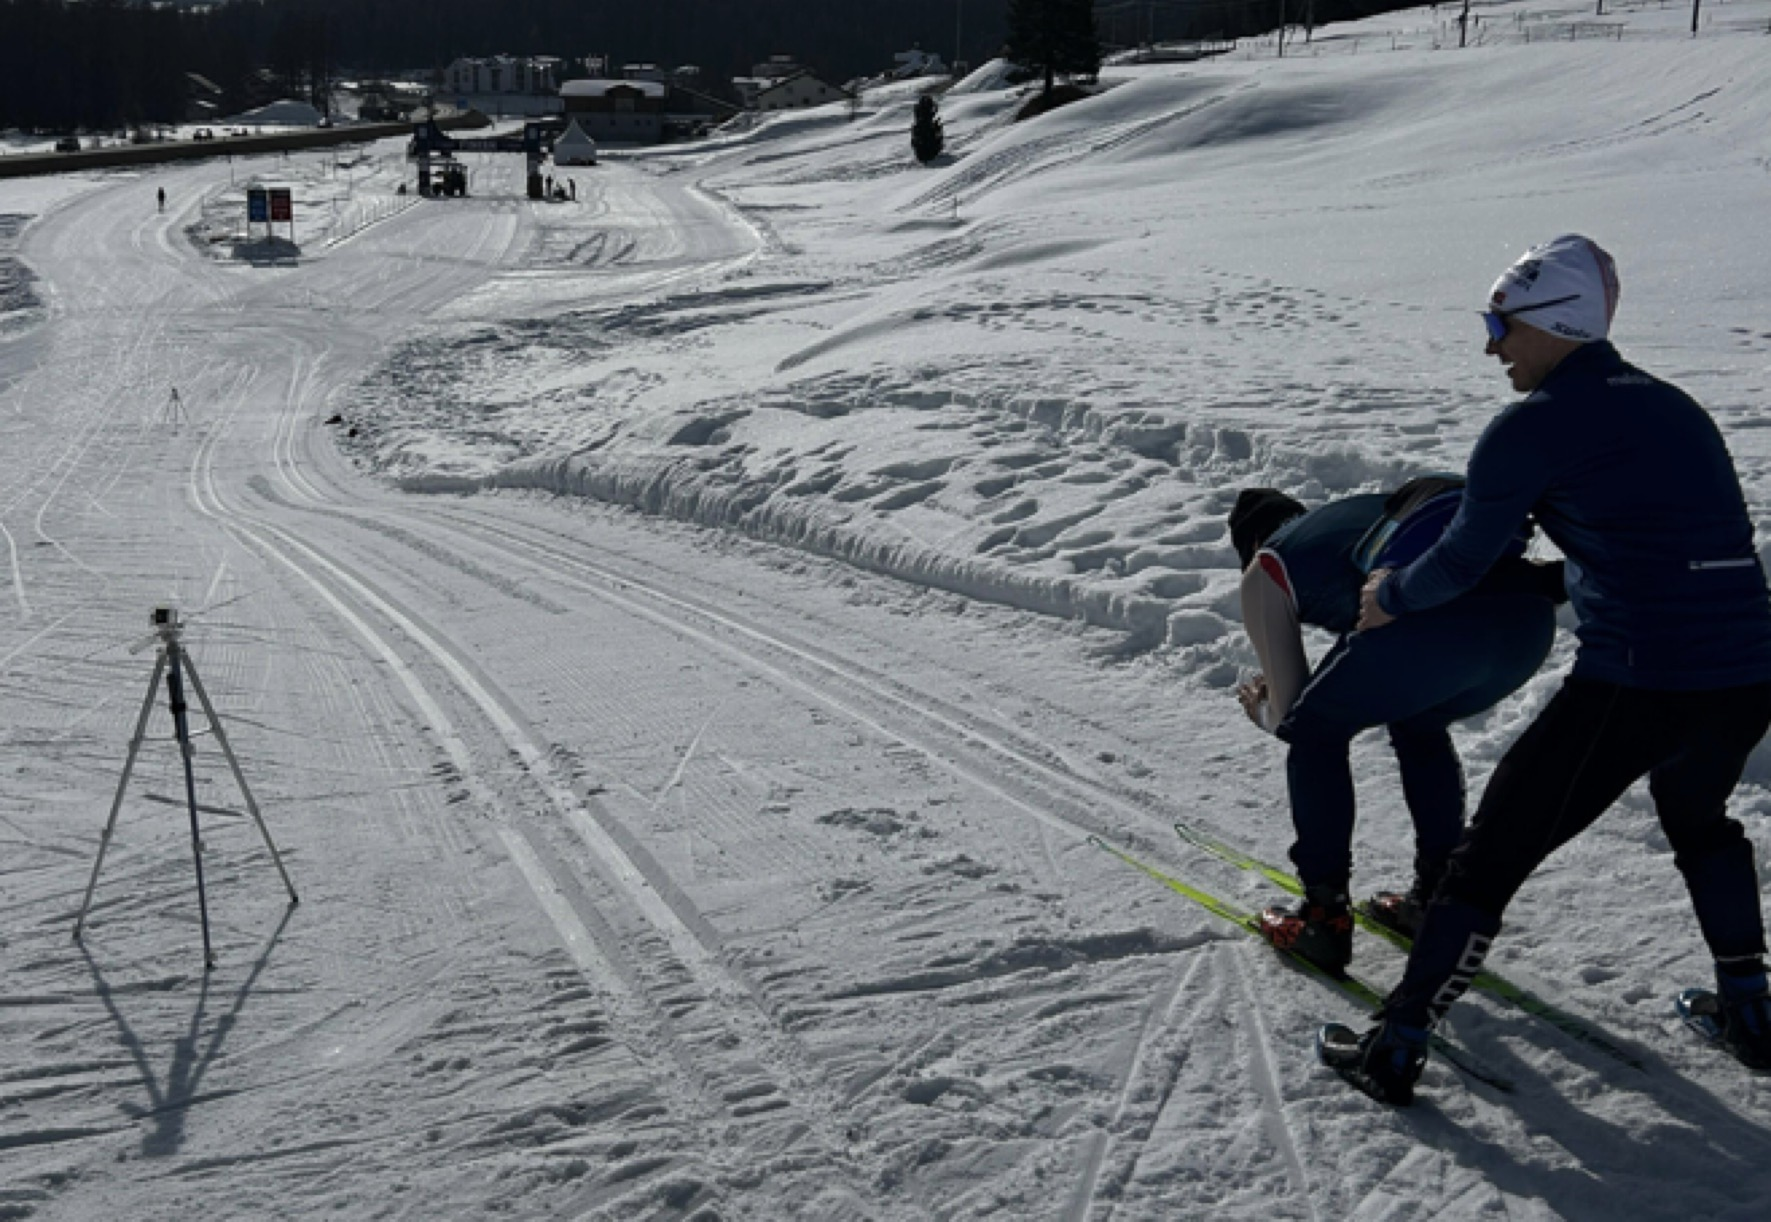
\includegraphics[width=0.9\linewidth]{Exp_2_Pontresina/Art-reelglobal-pontre.jpg}
    \caption{La position de départ: On voit à droite le skieur prêt en position de chouss, avec l'avant des fixations sur la ligne de départ. La personne qui le tient le lâche dans le moment qui suit. À gauche, le trépied avec le téléphone, qui est légèrement caché au milieu du trépied, qui enclenche le chronomètre. On aperçoit au pied de la pente le trépied avec le téléphone qui arrête le chronomètre.}
    \label{Pntre_global_art-sa}
\end{figure}

On remarque sur cette image une particularité au départ: en effet, la ligne de départ du skieur et le téléphone de départ sont légèrement décalés, ils ne sont pas à la même hauteur. Au fait, c'est logique que le départ soit contruit de cette manière: Vu que le chronomètre est enclenché par quelque chose qui passe la caméra, le skieur doit déjà être en mouvement lorsqu'il passe la borne de départ. Cela ne présente cependant pas de problème vu que tous les skieurs partent de la même ligne de départ.

\begin{figure}[H]
    \centering
    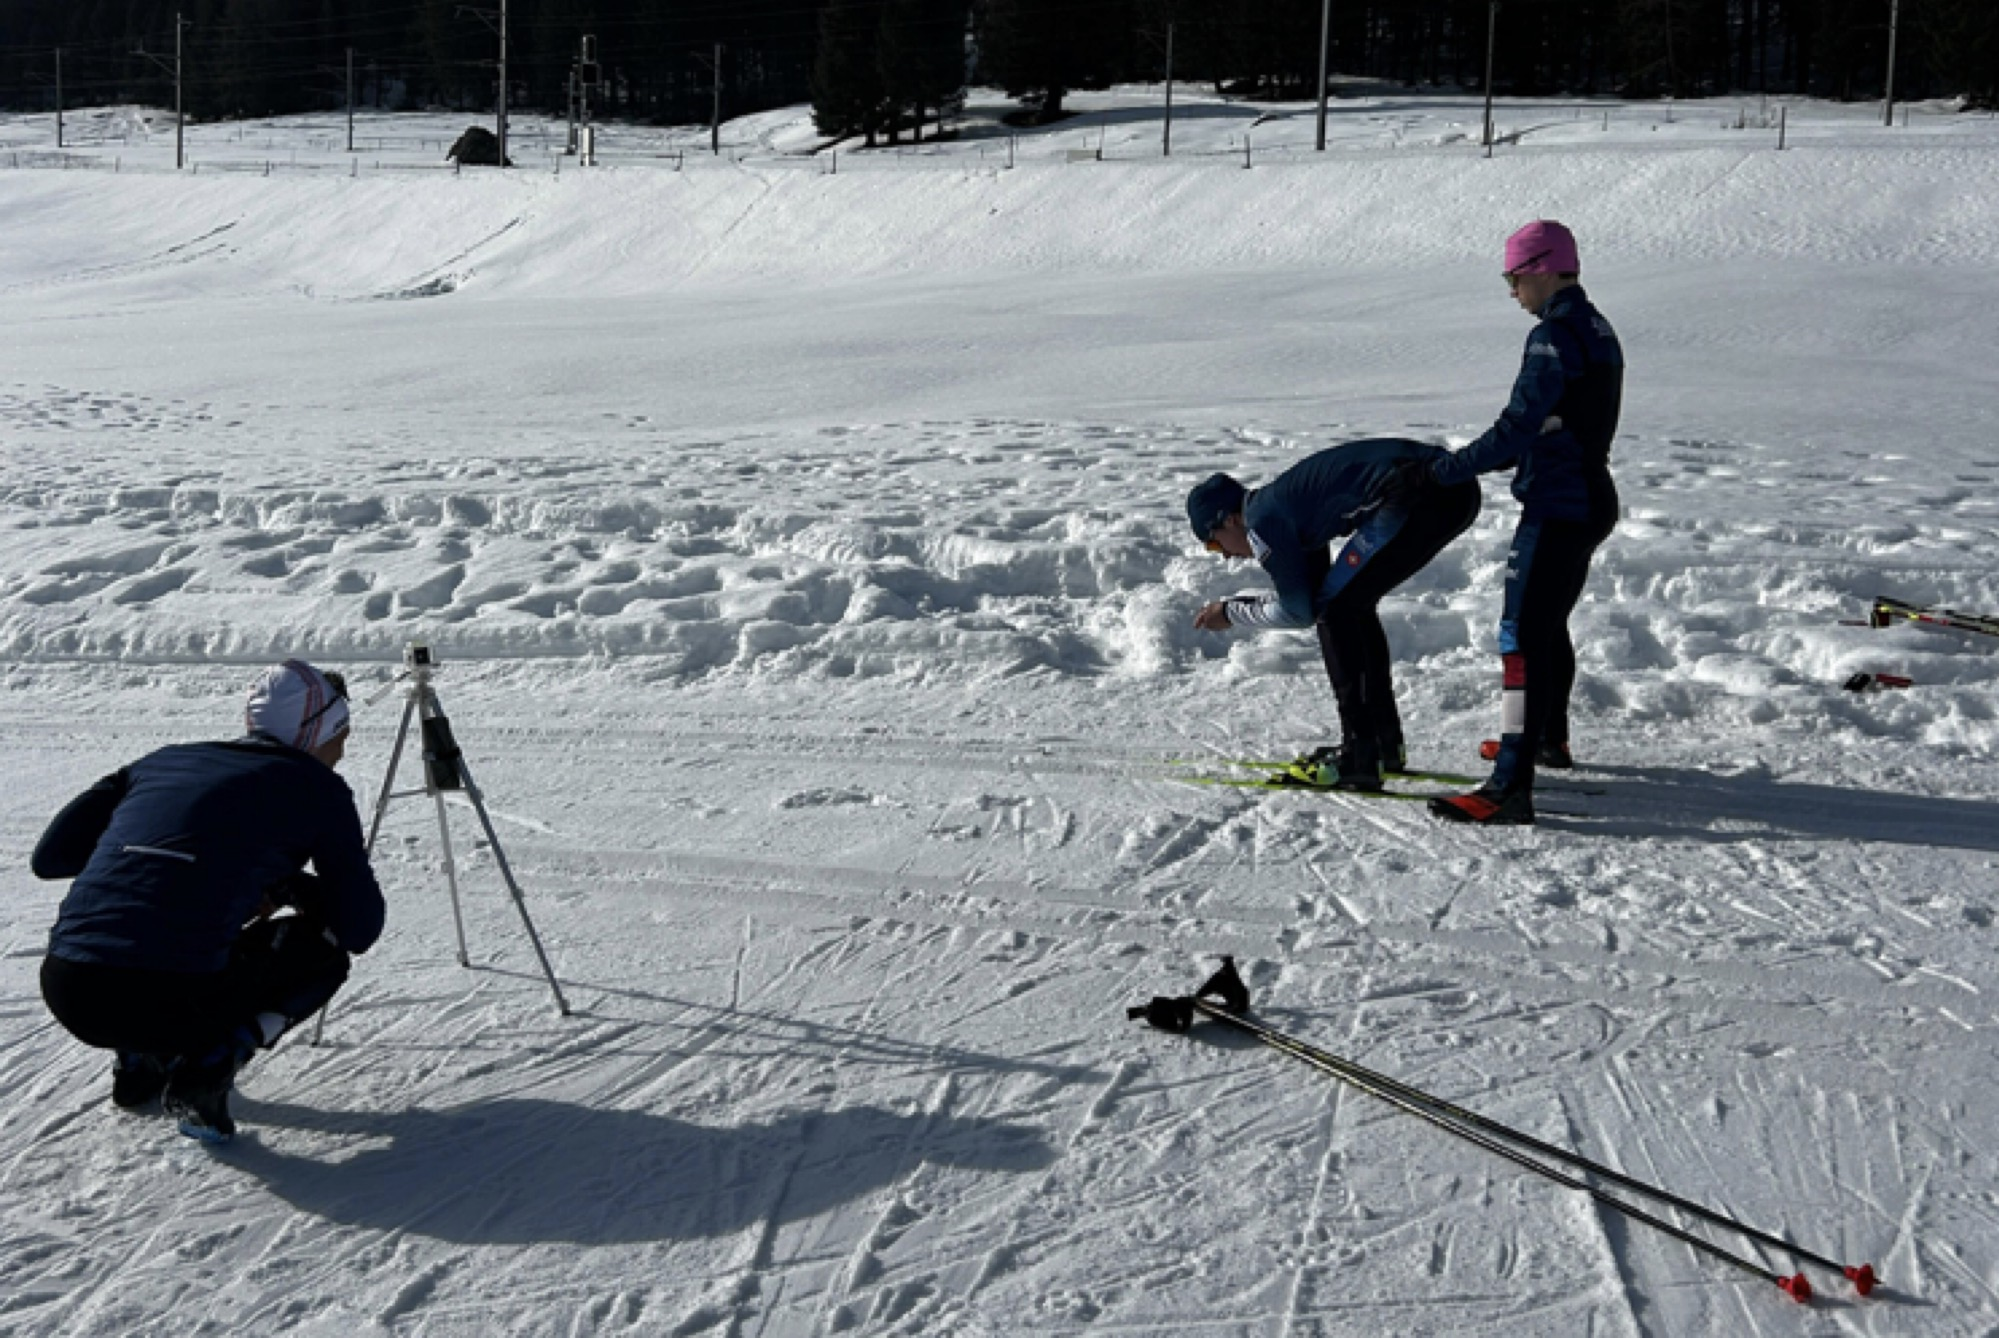
\includegraphics[width=0.9\linewidth]{Exp_2_Pontresina/Sit-start-global-pontre.jpg}
    \caption{Le départ en détail: On voit bien le décalge en tre le téléphone et le départ du skieur}
    \label{Pontre_start}
\end{figure}

Le départ du skieur ne correspond donc pas au départ du temps. On peut aussi le représenter sous forme de schéma:

\begin{center}
    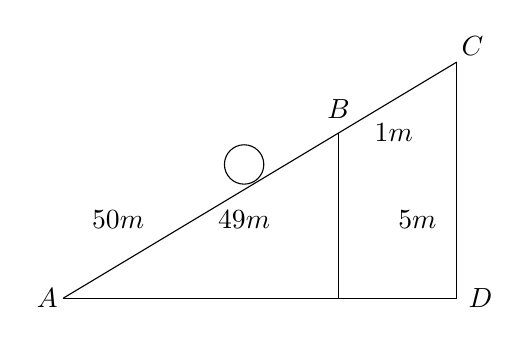
\begin{tikzpicture}
        \draw (1,0) -- (6,3);
        \draw (6,3) -- (6,0);
        \draw (4.5,2.1) -- (4.5,0);
        \draw (6,0) -- (1,0);
        \draw (3.3,1.7) circle (0.25);
            
                
        \draw node at (1.7,1) {$50m$};
        \draw node at (3.3,1) {$49m$};
        \draw node at (5.2,2.1) {$1m$};
        \draw node at (5.5,1) {$5m$};
        \draw node at (0.8,0) {$A$};
        \draw node at (4.5,2.4) {$B$};
        \draw node at (6.2,3.2) {$C$};
        \draw node at (6.3,0) {$D$};
    \end{tikzpicture}
\end{center}
\begin{itemize}
    \item où:
    \begin{itemize}
        \item $A$ est l'arrivée et l'arrêt du temps 
        \item $B$ est l'emplacement de la borne de départ et donc l'enclenchemet du temps
        \item $C$ est le départ du skieur
    \end{itemize}
\end{itemize}

Il y avait une petite imperfection dans la préparation et le déroulement: la différence de poids entre les skieurs. En effet, j'ai fait l'expérience avec mes amis et mon père, et nos poids allaient de $68[kg]$ à $79[kg]$, ce qui ne représente que $11[kg]$ de différence et un facteur de proportionnalité de $\sim 1.16$, ce qui est très peu. Nous avons donc dû faire les mesures en chouss avec que ces poids mais j'ai pu pour les mesures debout convaincre une personne de $50[kg]$ qui passait sur la piste de faire $4$ passages. Nous avons donc des mesures plus exhaustives debout qu'en chouss.

\subsubsection{Résultats et analyse (2)}

Voici donc les résultats dans la position chouss:

\begin{center}
\resizebox{1\textwidth}{!}{
    \begin{tabular}{|c|c|c|c|c|c|c|c|c|}
        \hline
        $M[kg]$&$t_1[s]$&$t_2[s]$&$t_3[s]$&$t_4[s]$& $t_5[s]$&$t_{moy}[s]$&Ince. abs.&Ince. prop. \\ \hline
        68     & 8,91	& 8,95	 & 8,87	  & 8,88   & 8,81	& 8,884 & 0,074 & 0,83296 \\ \hline
        70	   & 8,88	& 8,97	 & 8,91	  & 8,96   & 8,98	& 8,94 & 0,06 & 0,67114 \\ \hline 
        79	   & 8,77	& 8,77	 & 8,79	  & 8,73   & 8,75	& 8,762 & 0,032 & 0,36521 \\ \hline
        76	   & 8,81	& 8,69	 & 8,60	  & 8,69   & 8,68	& 8,694 & 0,116 & 1,33425 \\ \hline
    \end{tabular}
    }
\end{center}

\vspace{0.3cm}

Ce que l'on peut directement remarquer, est que les incertitudes proportionnelles sont toutes inférieures à $1.4 \%$, pour la plupart même inférieures à $1 \%$, ce qui prouve que le système de chronométrage fonctionne bien et aussi mieux que notre système à la première expérience. C'est aussi le cas pour les résultats debout:

\begin{center}
\resizebox{1\textwidth}{!}{
    \begin{tabular}{|c|c|c|c|c|c|c|c|}
    \hline
    $M[kg]$&$t_1[s]$&$t_2[s]$&$t_3[s]$&$t_4[s]$&$t_{moy}[s]$&Ince. abs.&Ince. prop.  \\ \hline
    76	   & 8,77	& 8,70	 & 8,67	  & 8,65   & 8,6975 & 0,0725 & 0,83357 \\ \hline
    79	   & 8,68	& 8,77	 & 8,71	  & 8,67   & 8,7075 & 0,0625 & 0,71777 \\ \hline
    70	   & 8,86	& 8,81	 & 8,82	  & 8,76   & 8,8125 & 0,0525 & 0,59574 \\ \hline
    68	   & 8,83	& 8,84	 & 8,80	  & 8,82   & 8,8225 & 0,0225 & 0,25503 \\ \hline
    50	   & 9,03	& 8,96	 & 8,93	  & 8,88   & 8,95   & 0,08 & 0,89385 \\ \hline
    \end{tabular}
    }
\end{center}

\vspace{0.3cm}

Les tableaux sont organisés en ordre chronologique, et un constat important à faire est que les temps moyens ne se réduisent pas dans l'ordre de passage. on peut donc dire que la source d'erreur principale de la première expérience a été, en tout cas en grande partie, éliminée.

\vspace{0.3cm}

On peut donc s'intéresser aux temps en fonction de la masse. Ici, il faut dire que les mesures en debout valent bien plus que celles en chouss, car il y a la personne plus légère que nous qui a créé un vrai écart de masse. 
\newline En effet, on ne remarque pas tout de suite sur les résultats en chouss que les personnes avec plus de masse sont plus rapides que les personnes avec moins de masse. Le skieur de $70[kg]$ par exemple est légèrement moins rapide que celui de $68[kg]$, et celui de $76[kg]$ est plus rapide que celui de $79[kg]$. Il faut ici cependant considérer le tableau d'ensemble: Les $2$ skieurs les plus lourds ont des temps bien plus rapides que les $2$ skieurs les plus légers. 
\newline Cela est déjà bien plus clair dans la position debout. En effet, on observe une réduction du temps avec la masse qui augmente, sauf encore une fois pour le skieur de $76[kg]$ et $79[kg]$. Cette réduction est d'un ordre de grandeur de $\sim 2.9\%$ entre le skieur de $50[kg]$ et celui de $76[kg]$, ce qui représente $1.74 [s]$ sur une descente de $1[min]$, pour donner une idée de l'ordre de grandeur. Ici, il est utile de mentionner que les skis que nous avons utilisés sont mes skis de compétition et que le skieur de $76[kg]$ est moi. Les skis sont donc ajustés pour moi (masse, position de la fixation, longueur, etc...), ce qui est une très légère source d'erreur. Je ne penses cependant pas que c'est la seule source d'erreur qui a produit cet effet.
\newline Un impact positif sur les résultats de faire cette expérience avec mes amis, est que $2$ personnes qui ont presque le même poids (les binômes de $70[kg]$-$68[kg]$ et $76[kg]$-$79[kg]$), permettent de "contrôler" la validité des résultats et que les sources d'erreurs ne sont pas trop grandes pour les biaiser. En effet, si les $2$ skieurs du même "binôme" avaient eu des temps complètement différents, les résultats seraient complètement décrédibilisés. 
\newline Tout cela est visible dans le graphique ci-dessous:

\begin{center}
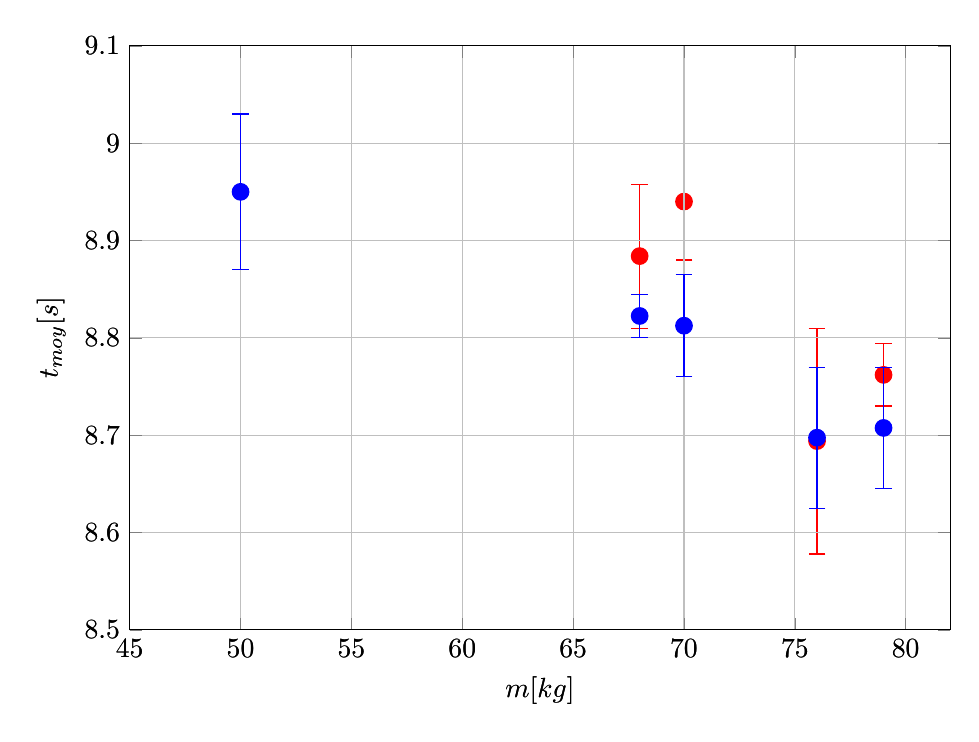
\begin{tikzpicture}
\begin{axis}[
    xlabel={$m [kg]$},
    ylabel={$t_{moy} [s]$},
    xmin=45, xmax=82,
    ymin=8.5, ymax=9.1,
    grid=both,
    width=12cm,
    height=9cm,
    mark size=3pt
]
\addplot[
    color = red,
    mark=*,
    only marks,
    error bars/.cd,
    y dir=both,
    y explicit,
] coordinates {
    (68,8.884) +- (0,0.074)
    (70,8.94)  +- (0,0.06)
    (76,8.694) +- (0,0.116)
    (79,8.762) +- (0,0.032)
};
\end{axis}
\begin{axis}[
    xlabel={$m [kg]$},
    ylabel={$t_{moy} [s]$},
    grid=both,
    width=12cm,
    height=9cm,
    xmin=45, xmax=82,
    ymin=8.5, ymax=9.1,
    mark size = 3pt
]
\addplot[
    color = blue,
    mark=*,
    only marks,
    error bars/.cd,
    y dir=both,
    y explicit,
] coordinates {
    (79,8.7075) +- (0,0.0625)
    (76,8.6975) +- (0,0.0725)
    (70,8.8125) +- (0,0.0525)
    (68,8.8225) +- (0,0.0225)
    (50,8.95)   +- (0,0.08)
};

\end{axis}
\end{tikzpicture}
\captionof{figure}{Le temps en fonction de la masse; En \textcolor{red}{rouge les mesures de chouss} et en \textcolor{blue}{bleu les mesures debout}}
\end{center}

Sur ce graphique, on voit visuellement très bien que l'écart de masse sur les mesures debout est plus du double de l'écart de masse sur les mesures en chouss. 
\newline On peut voir aussi que les $2$ séries de point ont au moins une tendance vers le bas, et que les points des $2$ binômes sont toujours relativement rapprochés, bien que la série de points \textcolor{blue}{bleue} a une baisse des temps bien plus linéaire que la \textcolor{red}{rouge}. Cela est probablement dû à la personne plus légère avec laquelle on peut plus donner un image d'ensemble, mais aussi au fait que la position réduit les sources d'erreurs par sa simplicité et son exposition plus grande à l'air. L'introduction de cette position a donc été un succès et donc la source d'erreur présente par la taille des skieurs est inférieure ou du moins pas supérieure à celle de la position de chouss. Nous allons donc garder les deux pour la prochaine expérience.

\vspace{0.3cm}

Il y a par contre une contradiction qui ressort quand on observe le graphique: Les temps en position debout sont plus rapides que les temps en chouss. Cela devrait cependant être l'inverse si l'on prend en compte les résistances de l'air. Au fait, cela est dû au départ un peu spécial: la position de départ est définie par l'avant des fixations qui sont sûr la ligne. Or, en chouss, le buste et la tête sont bien plus avancés par rapport aux pieds et la fixation. Après, au départ du temps, ce ne sont plus l'avant des fixations qui définissent le départ, mais le point le plus avancé du corps, donc la tête dans la plupart des cas. En étant debout cependant, le point le plus avancé du corps, donc le buste dans la plupart des cas, est presque aligné avec les pieds. Il y donc un décalage d'à peu près $0.5[m]$ de distance que parcours le skieur de la ligne de départ jusqu'à la borne de départ, entre les positions. Ce décalage fait que le skieur en position debout a déjà acquérit plus de vitesse que le skieur en position chouss quand il passe la borne de départ. Après, la distance sur laquelle nous avons mesuré le temps était sans doute trop courte pour que la difference dans les frottements de l'air rattrapent ce décalage. Si l'on reproduit donc cette expérience sur un parcours plus long, les temps de chouss devraient à un moment devenir plus rapides que les temps debout. 

\subsubsection{Sources d'erreurs à améliorer pour la prochaine expérience}

Bien que cette expérience ait été un succès et que les sources d'erreurs ont été significativement atténuées par rapport à la première, il y a quelques éléments qu'on peut changer pour la prochaine et dernière expérience:
\begin{enumerate}
    \item Les skis: Pour l'instant, nous n'avons utilisé que mes skis pour ces expériences. Bien que ce n'est pas une source d'erreur explicite, il serait intéressant pour la prochaine expérience de prendre des skis construits pour un personne plus légère par exemple.

    \item La longueur du parcours: J'aimerai bien faire une expérience sur une distance plus longue et peut-être aussi avec plus de pente pour voir si cela a un impact sur les résultats. En théorie, il devrait y avoir plus de difference avec plus de vitesse et plus de distance, car les forces de frottements du vent augmente exponentiellement avec la vitesse. Aussi, un plus grand temps de parcours va légèrement compenser les sources d'erreurs liées au chronométrage.

    \item La difference de poids: Il faudra pour la prochaine expérience prendre avec soi au moins une personne bien plus légère que nous et peut-être aussi ajouter du poids aux personnes les plus lourdes pour créer une plus grosse difference de poids.
\end{enumerate}

\subsubsection{Conclusion expérience 2}

En somme, cette expérience montre qu'\textbf{il y a en effet une augmentation générale de la vitesse avec la masse}, même si cette augmentation n'était pas présente entre absolument toutes les masses. Surout les résultats debout montrent cette augmentation de la vitesse, car la courbe des temps moyens est pas mal linéaire comparée à celle des résultats en chouss. Cette non-linéarité des séries de points montre qu'il existe toujours des sources d'erreurs, comme celle citée ci-dessus, ou des sources extérieures, comme par exemple le vent. De plus, cette augmentation n'est que de $\sim 2.9\%$ pour une augmentation du poids de $52\%$, ce qui n'est presque pas percevable en vie réelle.   
\subsection{3ème expérience}

La troisième expérience s'est déroulée au col des Mosses, le 21.03.2026. Il y avait du Soleil et un peu de vent, mais il ne soufflait pas très fort et nous avons choisi une piste à l'ombre.

\subsubsection{Préparation (3)}

La troisième expérience est essentiellement une reproduction de la deuxième, mais avec quelques subtilités:

\vspace{0.3cm}

Afin d'augmenter l'écart entre les masses, nous avons comme première mesure pris avec nous ma soeur, qui sera la masse légère.

\begin{minipage}{0.4\textwidth}
    \begin{center}
        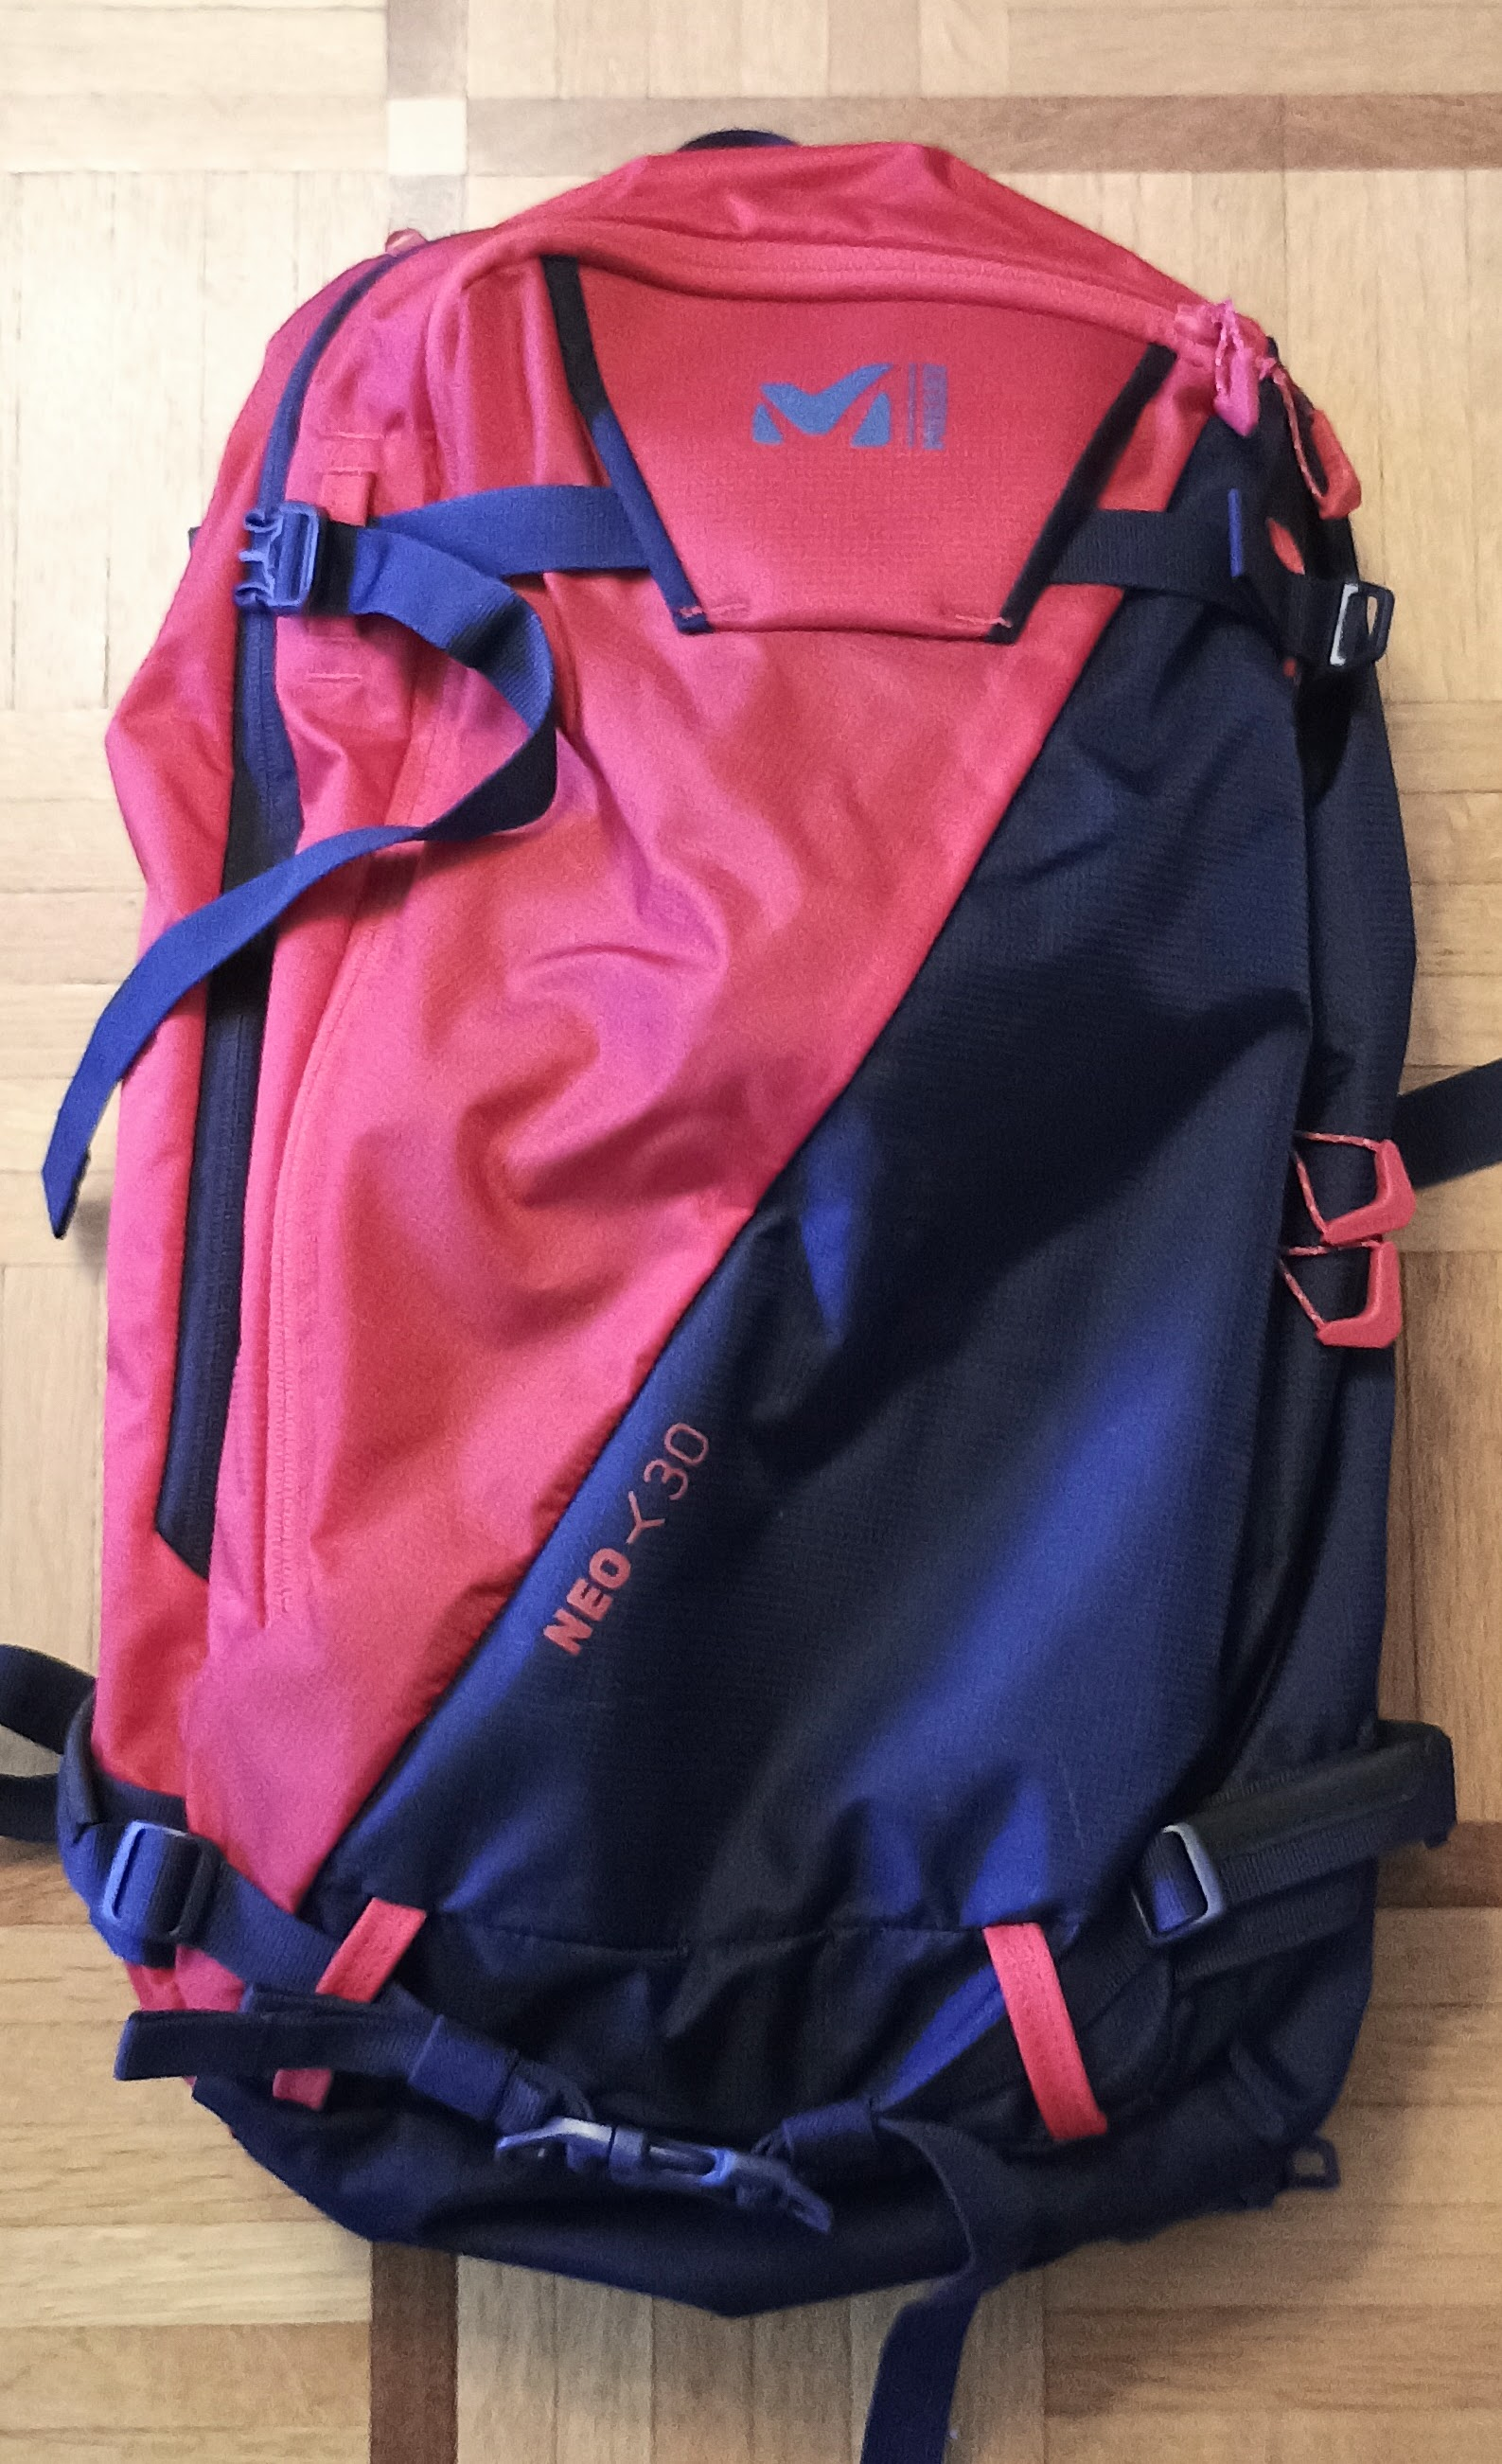
\includegraphics[width=0.8\textwidth]{Exp_3_Les-Mosses/Backpack_Laus.jpg}
        \captionof{figure}{le sac utilisé: il fallait choisir un sac qui supporte beaucoup de poids, mais qui n'est pas trop gros, car il fallait qu'il n'affecte pas trop l'aérodynamisme du skieur}
        \label{Backpack}
    \end{center}
\end{minipage}
\begin{minipage}{0.35\textwidth}
     Après, il fallait augmenter la masse maximale. Pour faire cela, nous avons tout simplement fait appel à un sac, et avons posés des poids dedans. Le sac avec les poids pesait $13[kg]$
     \vspace{0.2cm}
     Un autre changement a été la paire de ski utilisée: nous avons pris les skis qui appartiennent à ma soeur, qui sont construit pour son poids à peu près. Ces skis sont plus courts et ont moins de courbure. Ce sera intéressant de voir si cela a une influence sur les résultats.
\end{minipage}
\begin{minipage}{0.25\textwidth}
    \begin{center}
        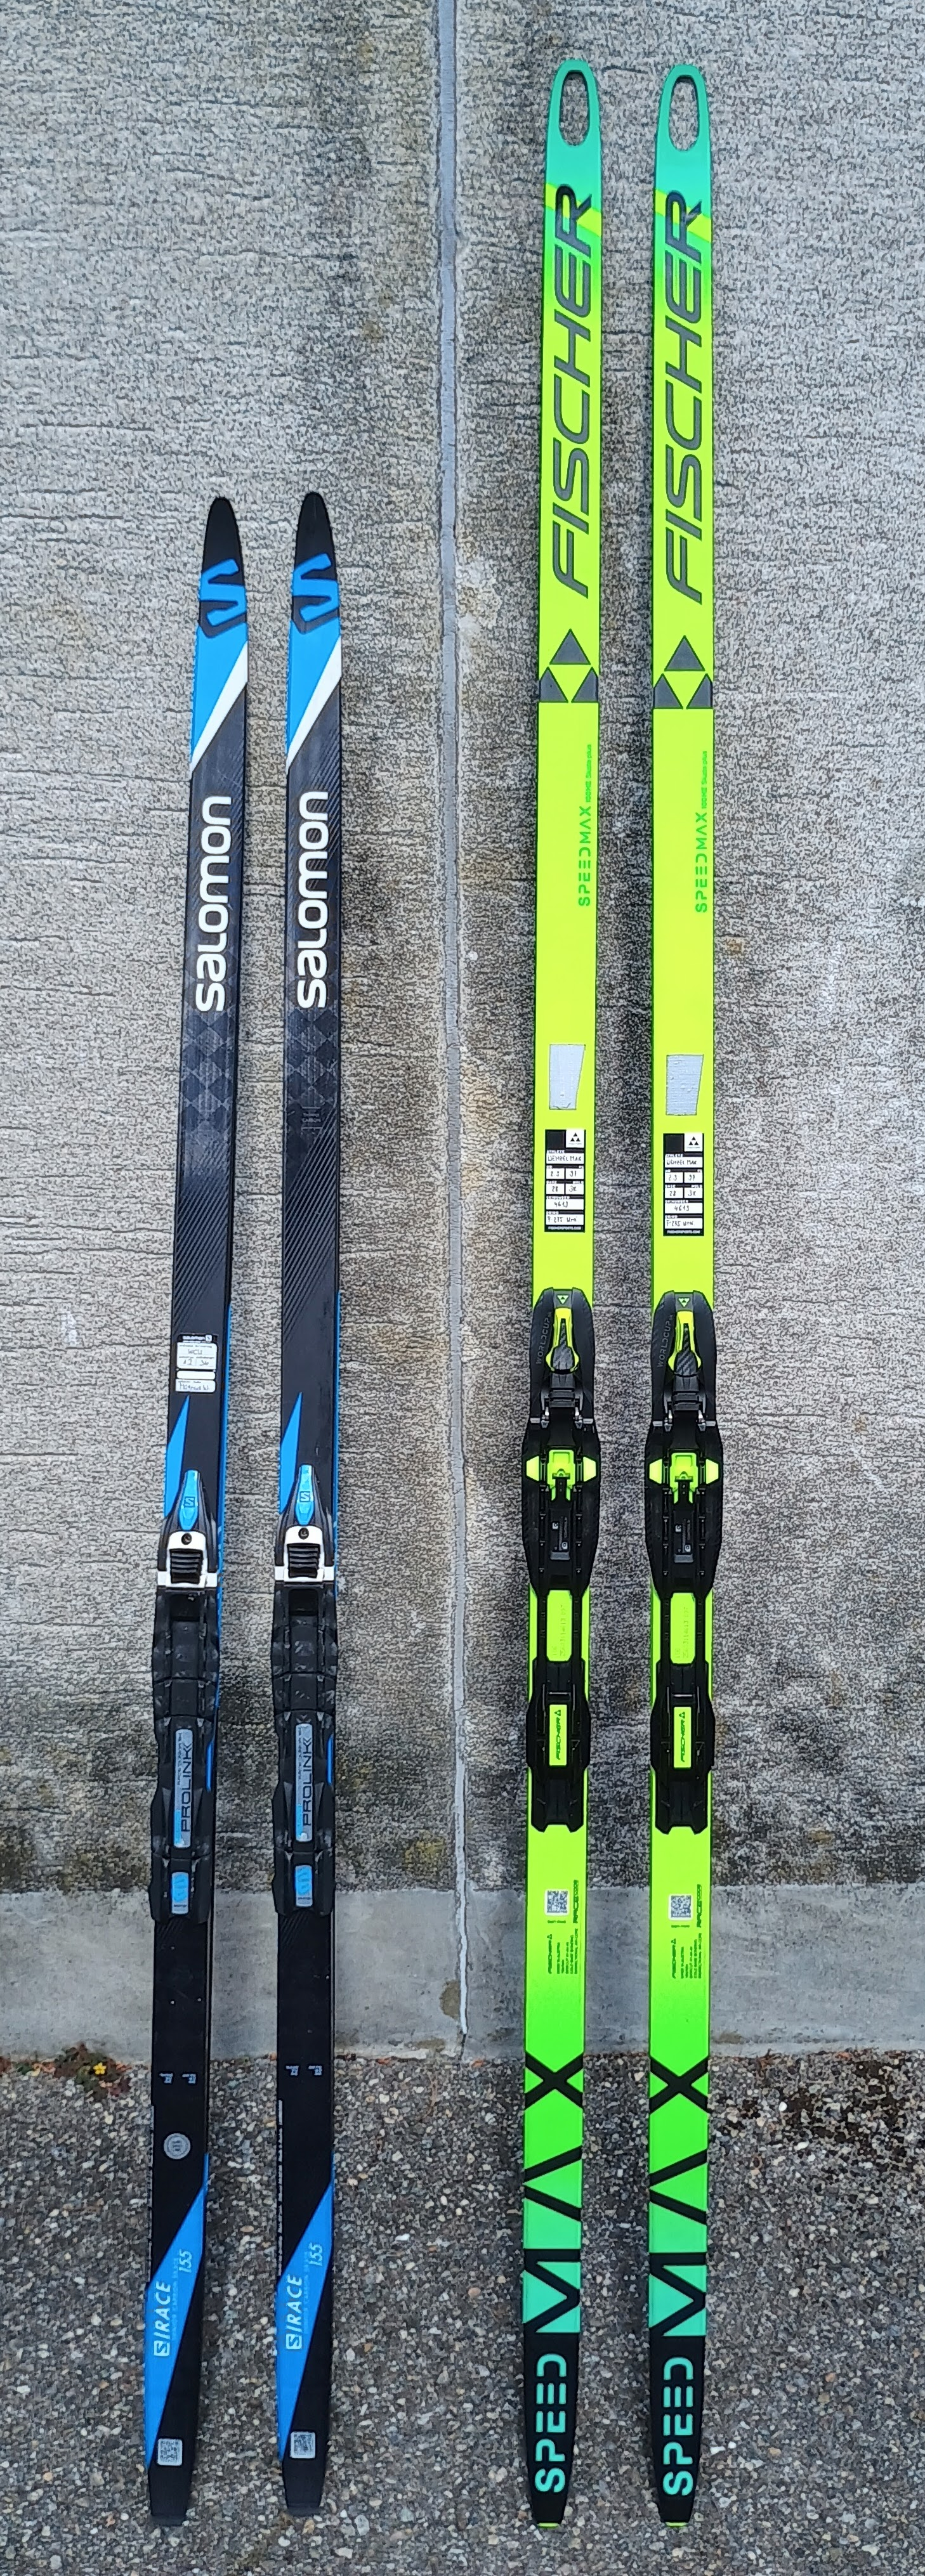
\includegraphics[width=0.8\textwidth]{Ski_surface_dry/Ski_both_comp_Laus.jpg}
        \captionof{figure}{Les deux skis utilisés: À gauche, le ski utilisé pour la $3^{eme}$ expérience, à droite, le ski pour les $2$ premières}
    \end{center}
\end{minipage}

\vspace{0.3cm}


\begin{minipage}{0.3\textwidth}
    \begin{center}
        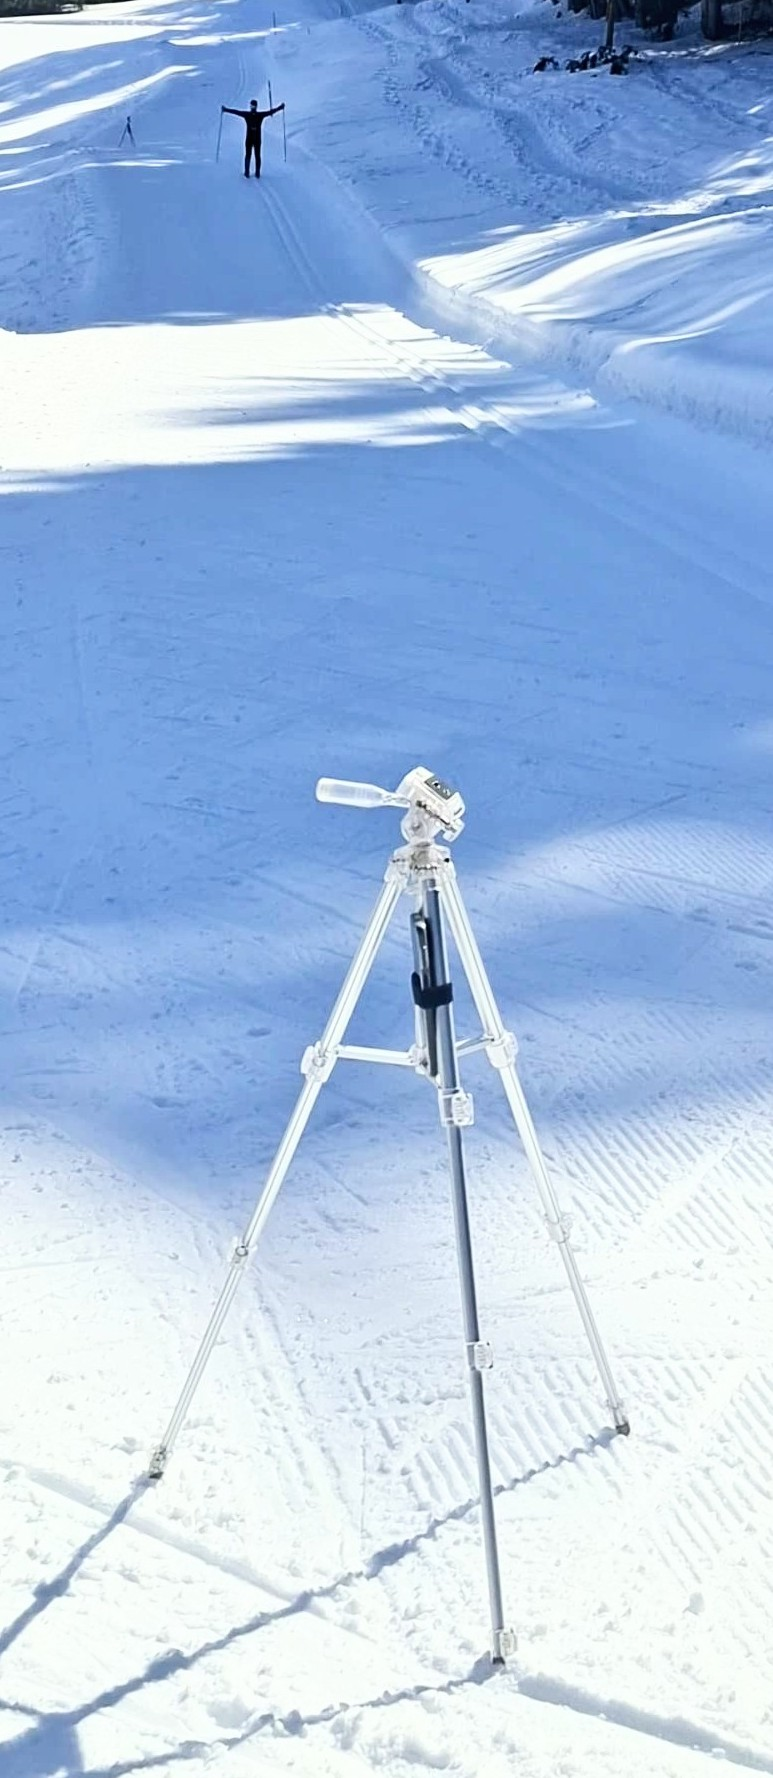
\includegraphics[width=0.7\linewidth]{Exp_3_Les-Mosses/Statif_deep_Lemoss.jpg}
        \captionof{figure}{La descente}
        \label{Statif_descente_lemoss}
    \end{center}
\end{minipage}
\begin{minipage}{0.7\textwidth}
    Une fois arrivé sur place, il a fallu trouver une pente appropriée sur laquelle faire l'expérience. Cela a été compliqué car il faisait chaud ce jour-là, il fallait donc une pente à l'ombre. De plus, nous voulions avoir une descente droite, longue et raide si possible. Notre choix est donc tombé sur une pente un peu spéciale par rapport aux $2$ autres expériences: elle a un angle au milieu et est coupée en $2$ parties. Le début est une partie raide, parfaite pour prendre de la vitesse, et la deuxième partie est un peu plus plate, mais aussi un petit peu plus longue.
    \newline Nous avons, une fois la descente trouvée et le système de chronométrage mis en place, fait plusieurs passages dans la trace de la descente jusqu'à ce que nos temps se stabilisent.
    \vspace{0.2cm}
    \newline On remarque sur la photo ci-contre que malgré le fait qu'il ait une ligne d'arbre au dessus de la piste qui procure de l'ombre, il y a quelques petites parties au milieu ensoleillées. Comme le soleil change d'emplacement dans le ciel le long d'une journée, ces "taches" se sont légèrement déplacées le long de la piste pendant toute l'expérience. Cela présente une légère source d'erreur.
\end{minipage}

\subsubsection{Déroulement (3)}

Comme dit plus haut, la troisième expérience est essentiellement une reproduction de la deuxième. Nous avons donc mis en place exactement le même système de chronométrage qu'à la deuxième expérience.
\begin{figure}[H]
    \centering
    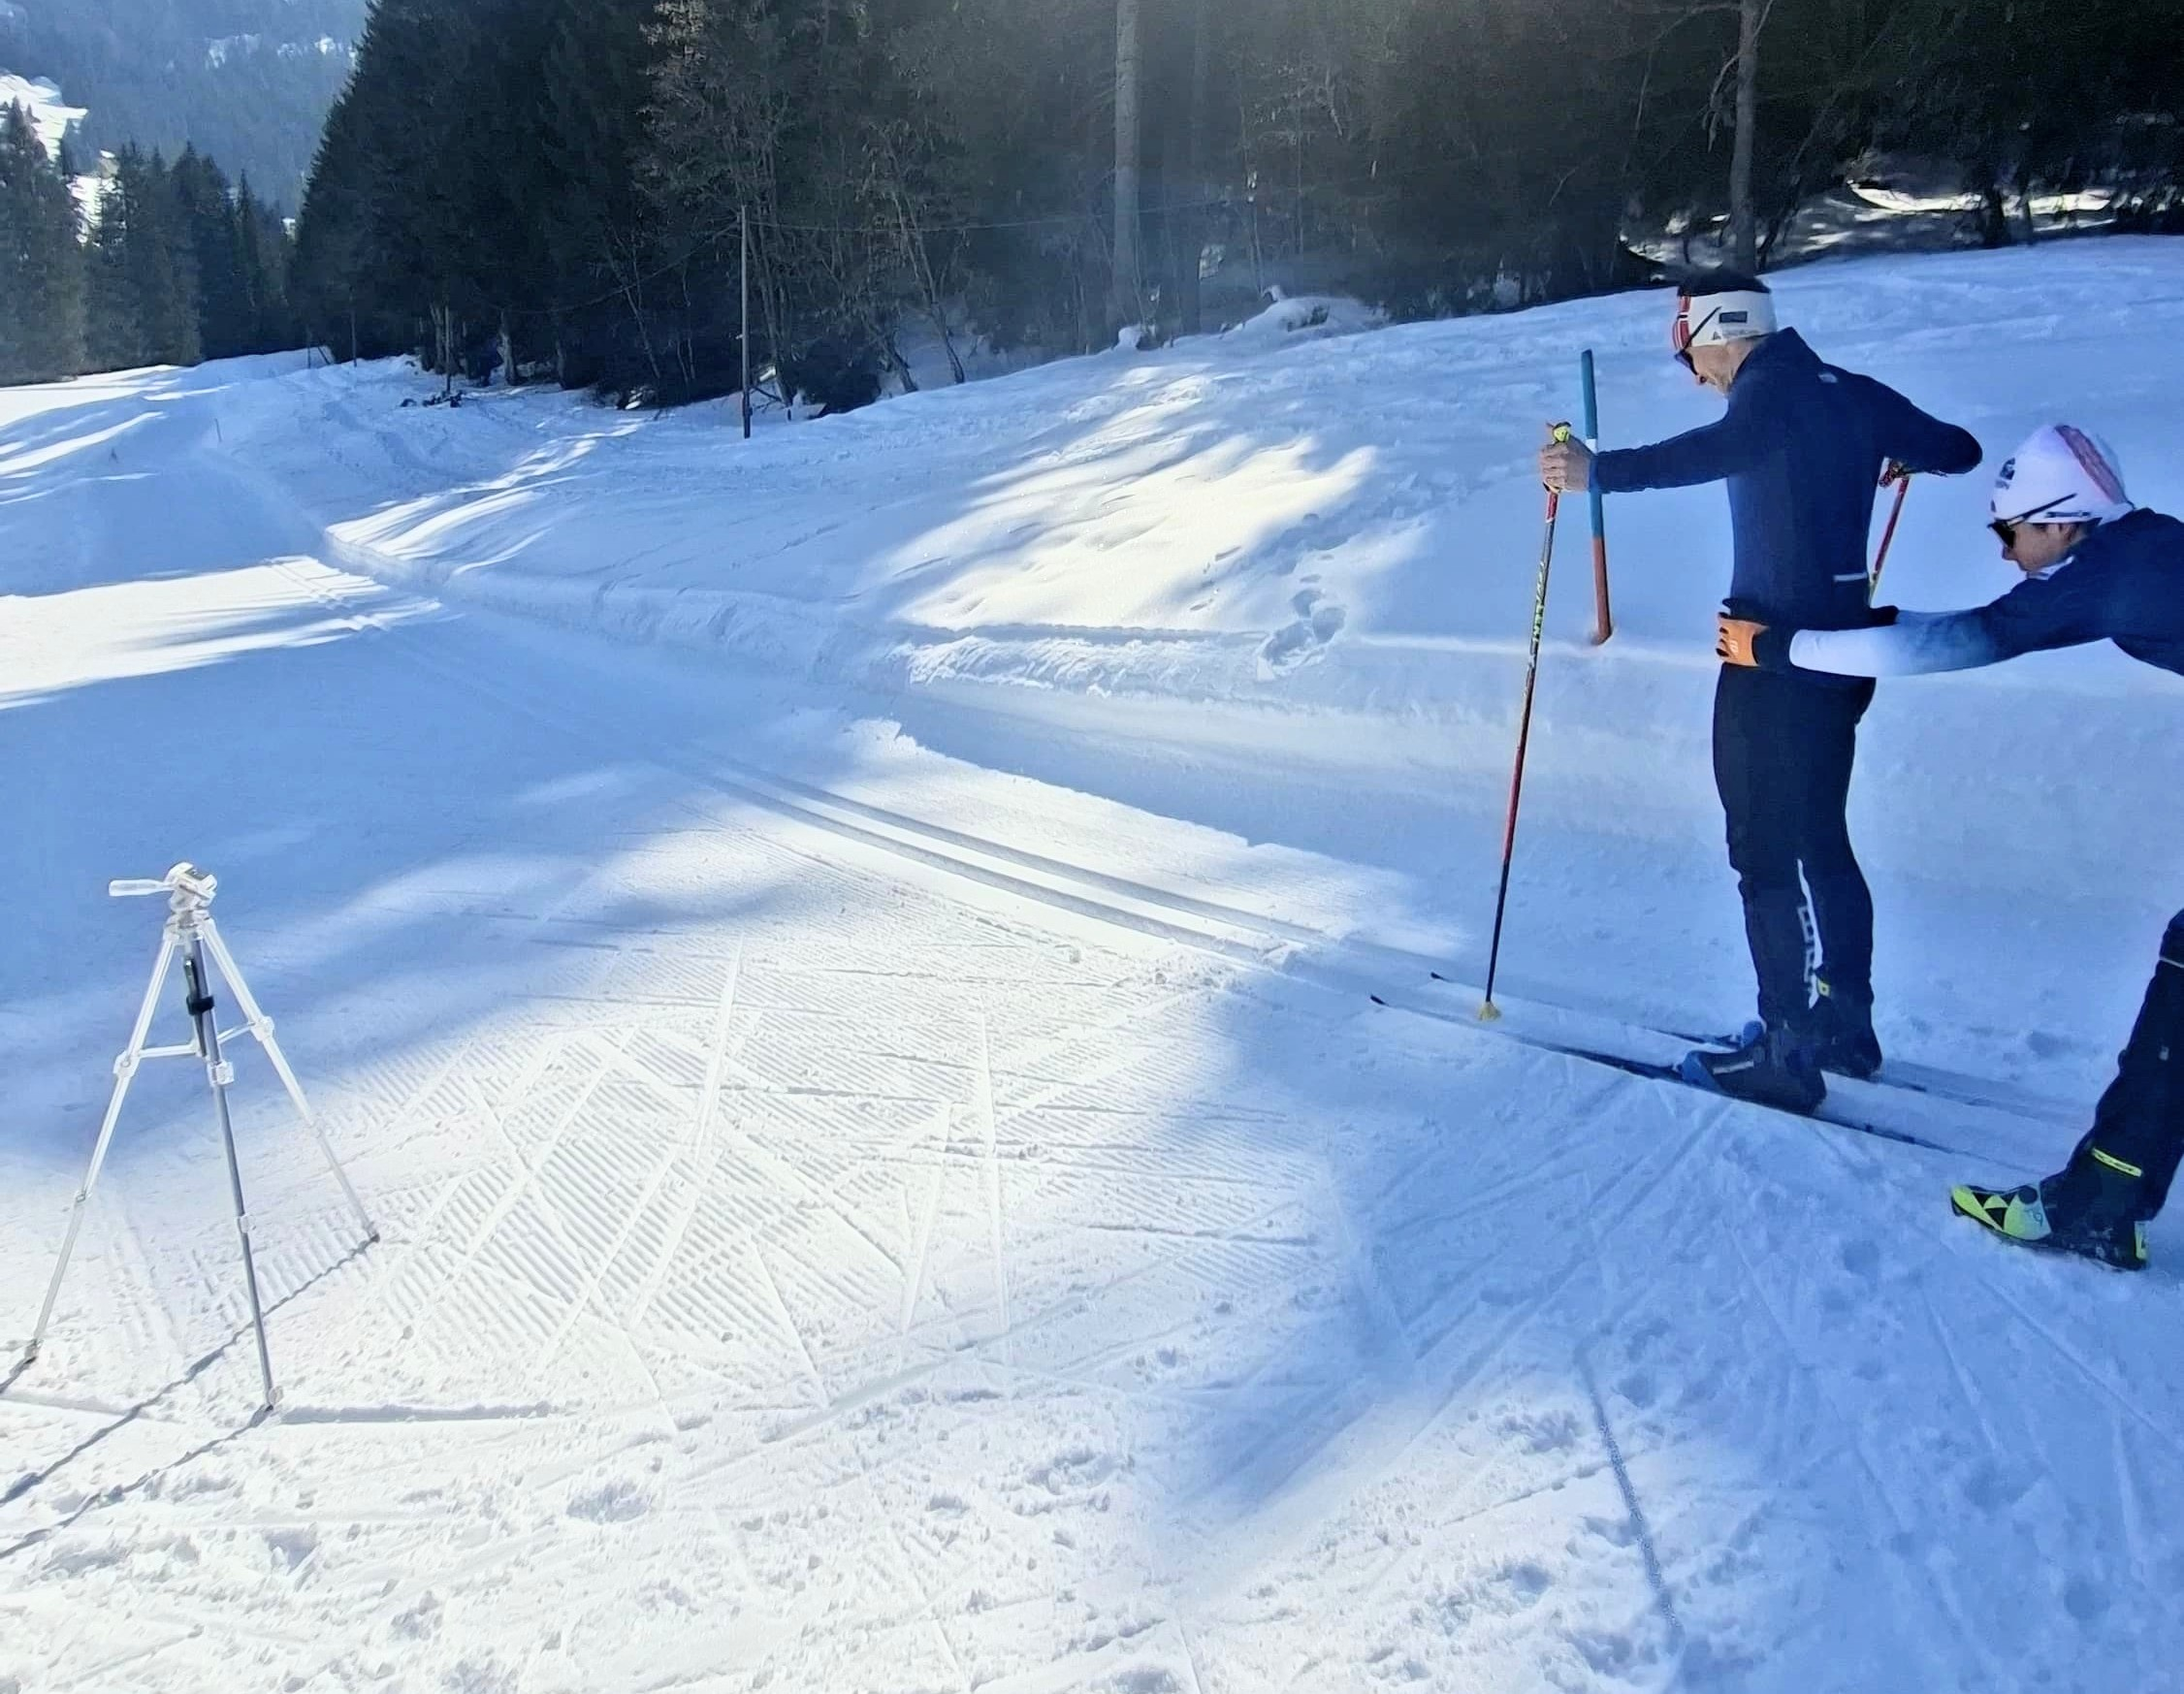
\includegraphics[width=0.8\linewidth]{Exp_3_Les-Mosses/Start_magpa_Lemoss.jpg}
    \caption{La piste avec le départ: À gauche, le trépieds avec le téléphone au milieu qui sert de borne de départ. On voit encore au loin la borne d'arrivée. À droite, le skieur, avec la personne qui tient le skieur derrière lui. Il est en-train de placer le skieur sur la ligne de départ, et le lâche quand il veut.}
    \label{start_lesmoss}
\end{figure}

J'aurai bien aimé installer une borne intermédiaire à l'angle de la piste, mais nous n'avions que $3$ téléphones, et il en fallait un pour prendre les photos. De plus, nous n'avions pas de troisième trépied.

\vspace{0.3cm}

Ici aussi, on peut établir un schéma avec toutes les distances aussi:

\begin{center}
    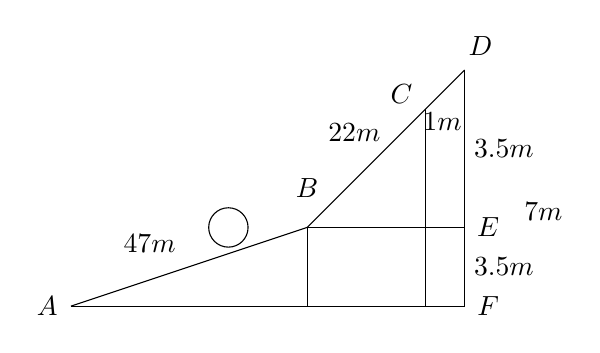
\begin{tikzpicture}
            \draw (1,0) -- (4,1);
            \draw (4,1) -- (4,0);
            \draw (4,1) -- (6,3);
            \draw (6,3) -- (6,0);
            \draw (5.5,2.5)-- (5.5,0);
            \draw (6,0) -- (1,0);
            \draw (4,1) -- (6,1);
            \draw (3,1) circle (0.25);
            
            \draw node at (2,0.8) {$47m$};
            \draw node at (4.6,2.2) {$22m$};
            \draw node at (7,1.2) {$7m$};
            \draw node at (5.72,2.35) {$1m$};
            \draw node at (6.5,2) {$3.5m$};
            \draw node at (6.5,0.5) {$3.5m$};
            \draw node at (0.7,0) {$A$};
            \draw node at (4,1.5) {$B$};
            \draw node at (5.2,2.7) {$C$};
            \draw node at (6.2,3.3) {$D$};
            \draw node at (6.3,1) {$E$};
            \draw node at (6.3,0) {$F$};
    \end{tikzpicture}
\end{center}

\begin{itemize}
    \item où:
    \begin{itemize}
        \item $A$ est l'arrivée et l'arrêt du temps
        \item $B$ est l'endroit ou la piste change de pente
        \item $C$ est l'emplacement de la borne de départ et l'enclenchement du temps
        \item $D$ est le départ du skieur
    \end{itemize}
\end{itemize}

La piste faisait donc en tout $69[m]$, ce qui est un peu plus long que les $2$ autres. La première partie de la pente a une inclinaison de $\sim 15.71\%$, ce qui est un peu plus raide que pour les $2$ autres expériences. La deuxième partie une pente de $\sim 7.43\%$.

\vspace{0.3cm}

Aussi, en partie à cause du fait que nous avons dû chercher une piste, nous n'avions encore moins de temps pour faire l'expérience qu'à la deuxième. Pour donc faire passer tout-le-monde et encore deux personnes avec le sac sur les deux expériences, nous n'avons seulement fait $3$ passages chacun. 
\newline Ensuite, pour varier un peu par rapport à la deuxième expérience, nous avons fait les passages debout d'abord et les passages en chouss après.


\subsubsection{Résultats et analyse (3)}

Voici donc les résultats debout:

\begin{center}
\resizebox{1\textwidth}{!}{
    \begin{tabular}{|c|c|c|c|c|c|c|}
        \hline
        $M[kg]$&$t_1[s]$&$t_2[s]$&$t_3[s]$&$t_{moy}[s]$&Ince. abs. $[s]$&Ince. prop. $[\%]$ \\ \hline
        47	& 10.83 & 10.79 & 10.75 & 10.79 & 0,04 & 0,37071 \\  \hline
        68	& 10.78 & 10.70	&       & 10.74	& 0,04 & 0,37244 \\	\hline
        70	& 10.79	& 10.74	& 10.51	& 10.68	& 0,17 & 1,59176 \\	\hline
        74	& 10.55	& 10.45	& 10.65	& 10.55	& 0,1 & 0,94768 \\	\hline
        81	& 10.62	& 10.54	& 10.55	& 10.57	& 0,05 & 0,47304 \\	\hline
        87	& 10.55	& 10.51	&	    & 10.53	& 0,02 & 0,18993 \\	\hline
    \end{tabular}
    }
\end{center}

\vspace{0.3cm}

La personne de $68[kg]$ et celle de $74[kg]$ sont celles qui ont aussi fait trois passages avec le sac. Les skieurs de $81[kg]$ et $87[kg]$ sont donc des skieurs alourdis. 
\newline Aussi, nous n'avons pas fait attention à mélanger les masses dans l'ordre de passage, mais n'avons pas non-plus fait exprès que l'ordre de passage correspond à l'ordre de masse des skieurs. Cela est une coïncidence.
\newline Nous avons malheureusement aussi oublié à inverser l'ordre de passage pour les mesures en chouss:

\begin{center}
\resizebox{1\textwidth}{!}{
    \begin{tabular}{|c|c|c|c|c|c|c|}
        \hline
        $M[kg]$&$t_1[s]$&$t_2[s]$&$t_3[s]$&$t_{moy}[s]$&Ince. abs. $[s]$&Ince. prop. $[\%]$ \\ \hline
        47	& 10.72	& 10.65	&	    & 10.685 & 0,035 & 0,32756 \\ \hline	
        70	& 10.58	& 10.54	& 10.59	& 10.57	 & 0,03 & 0,28382 \\ \hline
        74	& 10.51	& 10.51	& 10.45	& 10.49	 & 0,04 & 0,38131 \\ \hline
        87	& 10.51	& 10.44	&	    & 10.475 & 0,035 & 0,33413 \\ \hline	
    \end{tabular}
    }
\end{center}
\vspace{0.3cm}

La première chose qu'on remarque est bien sûr qu'il y a des mesures qui manquent, ce qui fait que, additionnellement au fait que nous n'avons que fait $3$ mesures pour tout-le-monde, il y en a vraiment peu pour quelques skieurs. Cela est très probablement dû au fait que les bornes de départ étaient assez loin l'un par rapport à l'autre, ce qui fait que la connexion bluetooth étaient très faible. Les $2$ téléphones ont donc sans doute dû perdre la connexion bluetooth pendant quelques secondes et pendant que le skieur passait une certaine borne. La conséquence est donc que cela présente une petite source d'erreur dans le fait que les temps moyens ne sont pas tant fiable que sur la deuxième expérience par exemple. 

\vspace{0.3cm}

Ensuite, il n'y a que $4$ mesures de skieurs pour les résulats en chouss, ce qui fait que encore une fois, les mesures de la position debout sont encore une fois plus exhaustives.

\vspace{0.3cm}

Ce qui est m'a surpris dans ces tableaux de mesure est que, contrairement à la deuxième expérience, les incertitudes pour les résultats en chouss sont cette fois tendanciellement plus petites que celles debout. Je n'ai pas d'explication exacte à cela mais il est possible que cela est aussi dû au conditions extérieures. Le vent, par exmeple, qui était légèrement plus présent que pendant les autres expériences, a potentiellement plus changé pendant les mesures debout que les mesures en chouss.

\vspace{0.3cm}

Finalement, on peut s'intéresser aux temps moyens. En effet, on peut observer que celui-là descend assez continuellement avec la masse, l'exception étant l'augmentation de temps du skieur alourdi de $81[kg]$ par rapport à celui de $74[kg]$. Le temps a été réduit de $\sim 2.47\%$ pour $\sim 85.1\%$ d'augmentation de masse sur les mesures debout et de $\sim 1.97\%$ pour toujours $\sim 85.1\%$ d'augmentation de la masse en chouss. Nous avons donc en effet légèrement plus de différence entre les masse sur la position debout, même si la différence de différence est petite. Par contre, il n'y a pas plus de réduction de temps qu'à la deuxième expérience, malgré différence de masse plus importante et le parcours plus long. Cela peut être dû à de nombreuses choses, comme par exemple encore une fois les conditions, où bien les skis plus petits. Peut-être que visualiser ces résultats aidera à encore mieux les comprendre, ou a en faire ressortir d'autres:

\begin{center}
    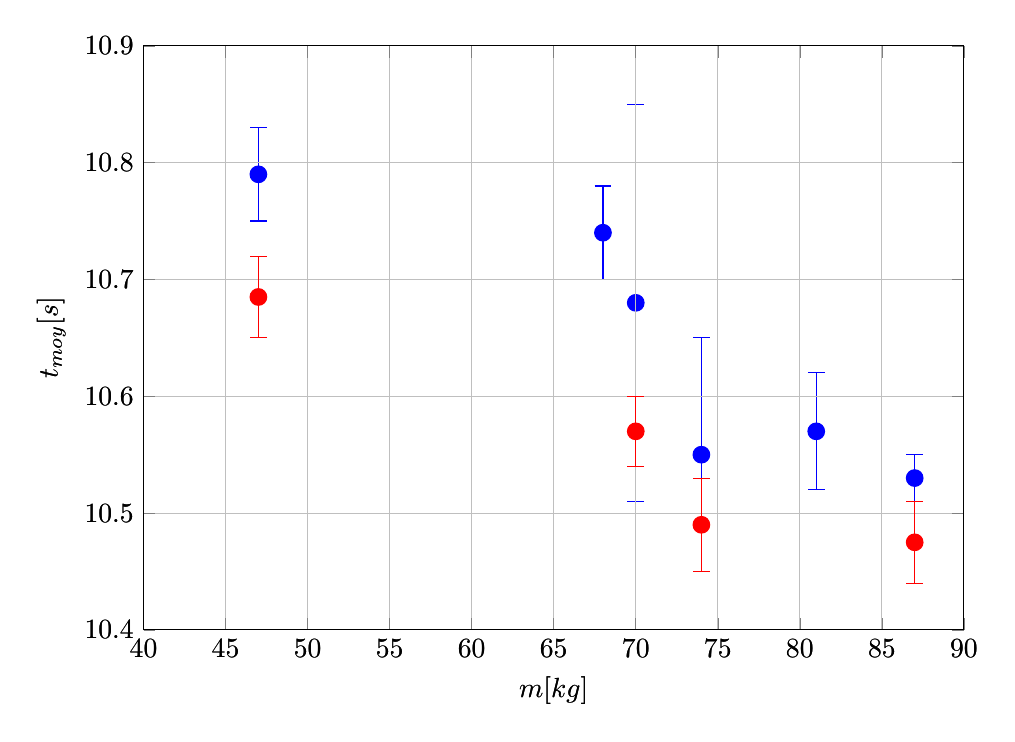
\begin{tikzpicture}
\begin{axis}[
    xlabel={$m [kg]$},
    ylabel={$t_{moy} [s]$},
    xmin=40, xmax=90,
    ymin=10.4, ymax=10.9,
    grid=both,
    width=12cm,
    height=9cm,
    mark size=3pt
]
\addplot[
    color = blue,
    mark=*,
    only marks,
    error bars/.cd,
    y dir=both,
    y explicit,
] coordinates {
    (47,10.79) +- (0,0.04)
    (68,10.74) +- (0,0.04)
    (70,10.68) +- (0,0.17)
    (74,10.55) +- (0,0.1)
    (81,10.57) +- (0,0.05)
    (87,10.53) +- (0,0.02)
};
\end{axis}
\begin{axis}[
    xlabel={$m [kg]$},
    ylabel={$t_{moy} [s]$},
    grid=both,
    width=12cm,
    height=9cm,
    xmin=40, xmax=90,
    ymin=10.4, ymax=10.9,
    mark size = 3pt
]
\addplot[
    color = red,
    mark=*,
    only marks,
    error bars/.cd,
    y dir=both,
    y explicit,
] coordinates {
    (47, 10.685) +- (0,0.035)	
    (70, 10.57)	+- (0,0.03)	
    (74, 10.49)	+- (0,0.04)	
    (87, 10.475) +-	 (0,0.035)	
};
\end{axis}
\end{tikzpicture}
\captionof{figure}{Le temps en fonction de la masse; En \textcolor{red}{rouge les mesures de chouss} et en \textcolor{blue}{bleu les mesures debout}}
\end{center}

En observant ce graphique, il y a $2$ possibles élements qui ressortent sur les $2$ séries de points qui peuvent justifier le fait que la réduction du temps est plus petite qu'à la deuxième expérience, alors que la difference de masse est plus grande:

\begin{enumerate}
    \item Le ski à ma soeur: En effet on voit que la pente des $2$ séries de points est bien plus raide que la pente entre le premier et deuxième point de chaque série. Je penses que c'est dû au fait qu'on ait pris les skis à ma soeur, faits pour son poids. Cela l'a rendue plus rapide ou les autres plus lents, relativement à la vitesse dans la deuxième expérience, faite avec mes skis. Après, à partir d'une certaine masse, la longueur du ski n'a probablement plus d'influence, car le ski touche de toute façon avec son intégralité la neige. Pour contrôler si la courbure et longueur du ski ont vraiment une influence sur les résultats, il faudrait faire cette expérience avec des skis faits exactements pour les poids à tout-le-monde, dont on sait qu'ils ont tous la même semelle, le même fart etc..
    
    \item Le sac alourdi: On voit le même phénomène "d'applatissement de la pente" sur les derniers points, et même une pente positive entre les $2$ derniers points sur la série de mesures debout. Pour rappel, les skieurs de $81[kg]$ sont $87[kg]$ avaient le sac sur eux. Justement, je penses que ce sac a légèrement affecté l'aérodynamisme des skieurs, et les a donc rendus plus lents, relatif à ce qu'un humain de la même taille et de même poids serait. Maintenant, alors que cela semble évident sur la position de chouss, on peut se demander comment cela affecte l'aérodynamisme sur la position debout, vu que le sac est normalement caché derrière le dos. Ici, on peut dire $2$ choses: premièrement, bien que le sac est derrière le dos, cela affecte quand même les petits tourbillons d'air autour d'un corps en mouvement et donc le coefficient de frottement $C$ (equation \ref{Airdrag}). Deuxièmement, il y a toujours les petits rubans, par exemple les rubans qui servent à ajuster la taille des manches (image \ref{Backpack}), qui flottent dans l'air et affectent l'aérodynamisme. 
\end{enumerate}

Il est bien sûr aussi possible que ces élements du graphique soient dû à des sources d'erreurs quelconques, mais le fait que la série des mesures en chouss soit quasiment parallèle à celle debout suggère qu'il y a des raisons assez précises.

\vspace{0.3cm}

Aussi, on remarque cette fois que les temps en chouss sont plus rapides que les temps debout. L'hypothèse qu'au bout d'un certain temps, les différences dans les forces de frottements de l'air compensent le décalage de vitesse au départ est donc juste.

\subsubsection{Sources d'erreurs en résumé}
Voici donc encore une fois les sources d'erreurs principales de cette expérience:
\begin{enumerate}
    \item Les skis: Comme mentionné plus haut, les skis qui sont faits pour des poids différents sont une possible source d'erreur. Pour l'éliminer, il faudrait exactement le même type de ski, mais faits pour des poids différents.

    \item L'alourdissement par le sac: Cet alourdissement a permit de créer un écart plus important entre les masses, mais a aussi influencé l'aérodynamisme des skieurs qui l'ont porté.

    \item Le jeu ombre-lumière sur le parcours: c'est sans doute la petite source d'erreur, mais elle est quand même présente, car elle a sans doute très légèrement modifié la neige de la piste au cours de  l'expérience.
\end{enumerate}


\subsubsection{Conclusion expérience 3}
En somme, cette expérience montre qu'\textbf{il y a en effet une augmentation générale de la vitesse avec la masse}, cette fois sur les $2$ séries de mesures. Cette réduction n'est cependant, inversement à ce que j'aurai attendu, pas plus grande et même légèrement plus petite que la réduction de temps à l'expérience précédente, ce qui est possiblement dû à des sources d'erreurs, comme les skis ou le sac.

\section{Conclusion}

Dans ce travail de maturité, nous avons vu qu'en théorie, si l'on prend les conditions extérieures en compte, la masse d'un skieur a en effet un impact sur la vitesse du skieur. Un skieur plus lourd qu'un autre devrait donc être plus rapide. 
\newline Tandis que la première expérience nous a surtout servi à pointer du doigt les sources d'erreurs à éviter, la deuxième et troisième ont confirmé expérimentalement qu'il y a bien une augmentation de la vitesse avec la masse. Cette augmentation cependant, que nous avons mesurée par réduction du temps, est tellement petite qu'elle est à mon avis non-perceptible par des skieurs. Je pense que d'autres facteurs, comme la relance au début d'une descente, la trajectoire, la technique de descente et l'aspiration sont immensement plus important pour déterminer la vitesse dans la descente que la masse du skieur. On peut donc conclure que la phrase "Il était aussi rapide que moi dans les descentes, alors que je suis plus lourd que lui, j'avais donc forcément de moins bons skis" est invalide, malgré les résultats que nous avons obtenus.

% %
% \section{Unités}
% Voici un sommaire des unités utilisées:
% \begin{itemize}
%     \item $[m]$: le Mètre, unité de distance
%     \item $[m^2]$: Le Mètre carré, unité de surface
%     \item $[m^3]$: Le Mètre cubique, unité de volume
%     \item $[s]$: la Seconde, unité de temps
%     \item $[\frac{m}{s}]$: Le Mètre par Seconde, unité de vitesse
%     \item $[\frac{m}{s^2}]$: Le Mètre par Seconde au carré, unité d'accélération
%     \item $[kg]$: Le Kilogramme, unité de masse
%     \item $[\frac{kg}{m^3}]$: Les Kilogrammes par Mètre cube, unité de masse volumique
%     \item $[N]$: le Newton, unité de force
%     \item $[^\circ]$: Le Degré, unité d'angle
%     \item $[Pa]$: Le Pascal, unité de pression
%     \item $[K]$: Le Kelvin, unité de température
%     \item $[\frac{m^3}{mol}]$: Les mètres cubes par mole, unité de volume molaire
%     \item $[\frac{J}{mol}]$: Les Joules par mole, unité d'enthalpie de fusion molaire    
% \end{itemize}
%


\bibliographystyle{unsrt}
\bibliography{Sandberg_COD_2025}

\end{document}
